
%To Print Notes too
%\documentclass[11pt, notes]{beamer}

%To Compile Only slides
\documentclass[11pt]{beamer}

\usepackage{amsmath,amsthm,enumerate,graphicx,bm,type1cm,amssymb,epsfig,lscape,setspace,url,listings,color,float}
%wrapfig,tikz,calc}
\usepackage{fancybox,etoolbox}
\usepackage{hyperref}
\usepackage[round]{natbib}
%\usepackage{soul}

%\setstcolor{red}

\usepackage[normalem]{ulem}
\usepackage{xcolor}


\newcommand\redsout{\bgroup\markoverwith{\textcolor{red}{\rule[0.5ex]{2pt}{0.4pt}}}\ULon}


% % %%FOR PRINTING
%\usepackage{pgfpages}
%\pgfpagesuselayout{2 on 1}[letterpaper,border shrink=5mm]
% % %%\pgfpagesuselayout{resize to}[letterpaper,border shrink=5mm,landscape]
%


%\setlength{\oddsidemargin}{5mm}
%\setlength{\textwidth}{16cm}
%\setlength{\topmargin}{0pt}
%\setlength{\headheight}{0pt}
%\setlength{\headsep}{0pt}
%\setlength{\textheight}{23cm}
%\onehalfspacing
%\setbeamersize{text margin left = 10pt}




\usetheme{Madrid}

% \definecolor{lightblue}{rgb}{.4,.4,1}
% \definecolor{babyblue}{rgb}{0.54, 0.81, 0.94}
%\definecolor{blizzardblue}{rgb}{0.67, 0.9, 0.93}
	\definecolor{columbiablue}{rgb}{0.61, 0.87, 1.0}
\definecolor{deepskyblue}{rgb}{0.0, 0.75, 1.0}
	\definecolor{electricblue}{rgb}{0.49, 0.98, 1.0}
\definecolor{lightskyblue}{rgb}{0.53, 0.81, 0.98}
\definecolor{skyblue}{rgb}{0.53, 0.81, 0.92}
 \definecolor{unc}{rgb}{0.2, 0.7, 1.0}
 \definecolor{unc}{rgb}{0.2, 0.75, 1.0}
 % \colorlet{beamer@blendedblue}{deepskyblue!100!black}
 \colorlet{beamer@blendedblue}{unc!95!black}

\setbeamersize{text margin left=1em}
\beamertemplatenavigationsymbolsempty

%\usetheme{Frankfurt}
%\useoutertheme{smoothtree}
%\useinnertheme{circles}


%\sectionfont{\large}

%\theoremstyle{definition}
%\newtheorem{mc}{MC}
%\newtheorem{thm}{Theorem}[section]
%\newtheorem{example}{Example}[section]
%\newtheorem{prop}{Proposition}[section]
%\newtheorem{pr}{Proof}
%\newtheorem{assump}{Assumption}[section]
%\newtheorem{lemma}{Lemma}[section]
%\newtheorem{definition}{Definition}[section]
%\newtheorem*{dfn}{Definition}
%\newtheorem*{rem}{Remark}
% \def\stackunder#1#2{\mathrel{\mathop{#2}\limits_{#1}}}
% \renewcommand{\theequation}{\thesection.\arabic{equation}}
%\newtheorem{corol}{Corollary}[section]

\undef{\lemma}
\newtheorem{lemma}{Lemma}

\undef{\assumption}
\newtheorem{assumption}{Assumption}

\undef{\remark}
\newtheorem{remark}{Remark}

\undef{\corollary}
\newtheorem{corollary}{Corollary}

\undef{\example}
\newtheorem{example}{Example}

\newtheorem{model}{Model}
  

\setlength{\bibsep}{0pt plus 0.3ex}

\allowdisplaybreaks

\restylefloat{table}

\newcommand{\beginbackup}{
   \newcounter{framenumbervorappendix}
   \setcounter{framenumbervorappendix}{\value{framenumber}}
}
\newcommand{\backupend}{
   \addtocounter{framenumbervorappendix}{-\value{framenumber}}
   \addtocounter{framenumber}{\value{framenumbervorappendix}} 
}



\DeclareMathOperator{\plim}{plim}
%\DeclareMathOperator{\argmin}{argmin}
\DeclareMathOperator{\arginf}{arginf}
\DeclareMathOperator{\argsup}{argsup}
\DeclareMathOperator{\var}{var}

\newcommand{\pmat}[1]{\begin{pmatrix} #1 \end{pmatrix}}
\newcommand{\argmax}{\mathop{\rm argmax \ }\limits}
\newcommand{\argmin}{\mathop{\rm argmin \ }\limits}
%\newcommand{\var}{\mathop{\rm var }}
\newcommand{\cov}{\mathop{\rm cov }}
\newcommand{\vecop}{{\rm vec}}

\newcommand{\Bb}{\mathbb{B}}
\newcommand{\R}{\mathbb{R}}
\newcommand{\N}{\mathbb{N}}
\newcommand{\Prob}{\mathbb{P}}


\newcommand{\A}{\mathcal{A}}
\newcommand{\B}{\mathcal{B}}
\newcommand{\C}{\mathcal{C}}
\newcommand{\D}{\mathcal{D}}
\newcommand{\E}{\mathcal{E}}
\newcommand{\F}{\mathcal{F}}
\newcommand{\G}{\mathcal{G}}
\newcommand{\He}{\mathcal{H}}
\newcommand{\Hs}{\mathcal{H}}
\newcommand{\Is}{\mathcal{I}}
\newcommand{\J}{\mathcal{J}}
\newcommand{\K}{\mathcal{K}}
\newcommand{\Le}{\mathcal{L}}
\newcommand{\M}{\mathcal{M}}
\newcommand{\Ns}{\mathcal{N}}
\newcommand{\Pc}{\mathcal{P}}
\newcommand{\Rs}{\mathcal{R}}
\newcommand{\Ss}{\mathcal{S}}
\newcommand{\Tc}{\mathcal{T}}
\newcommand{\Ts}{\mathcal{T}}
\newcommand{\U}{\mathcal{U}}
\newcommand{\V}{\mathcal{V}}
\newcommand{\W}{\mathcal{W}}
\newcommand{\X}{\mathcal{X}}
\newcommand{\Y}{\mathcal{Y}}
\newcommand{\Z}{\mathcal{Z}}

\newcommand{\qv}[2]{\langle #1 \rangle_{#2}}
\newcommand{\del}{\triangledown}
\newcommand{\deriv}[1]{\frac{\partial}{\partial #1}}
\newcommand{\derivn}[2]{\frac{\partial^{#2}}{\partial {#1}^{#2}}}
\newcommand{\e}{\varepsilon}
\newcommand{\T}{\tau}
\newcommand{\Tv}{\vec{\tau}}
\newcommand{\tod}{\xrightarrow{d}}
\newcommand{\toP}{\xrightarrow{p}}
\newcommand{\toas}{\xrightarrow{as}}

\newcommand{\pcite}[1]{\citeauthor{#1}'s (\citeyear{#1})}
\newcommand{\highlight}[1]{{\color{red} #1}}
\newcommand\blfootnote[1]{%
	\begingroup
	\renewcommand\thefootnote{}\footnote{#1}%
	\addtocounter{footnote}{-1}%
	\endgroup
}



\usepackage{xcolor}
\colorlet{red1}{red!80!blue!80}
\colorlet{green1}{green!80!black}
\colorlet{blue1}{blue!30}
\def\bxht{\dimexpr1.5\baselineskip\relax}
\def\bxwd{\dimexpr0.7in\relax}
\newcommand\cbox[2][\bxwd]{\def\boxwidth{#1}\def\boxcolor{#2}\cboxX}
\newcommand\cboxx[2][\bxwd]{\def\boxwidth{#1}\def\boxcolor{#2}\cboxXX}
\newcommand\cboxX[2][white]{\colorbox{\boxcolor}{%
  \rule[-.5\dimexpr\bxht-.7\ht\strutbox]{0pt}{\bxht}%
  \parbox[c]{\boxwidth}{\small\centering\color{#1}#2}}}
\newcommand\cboxXX[2][black]{\colorbox{\boxcolor}{%
  \rule[-.5\dimexpr\bxht-.7\ht\strutbox]{0pt}{\bxht}%
  \parbox[c]{\boxwidth}{\small\centering\color{#1}#2}}}



\title[Max Test under id Failure] % (optional, only for long titles)
{Testing Many Parameters under Mixed Identification Strength 
}
\author[Jay Dennis] % (optional, for multiple authors)
{Jay Dennis
}
\institute[UNC-CH]{UNC Chapel Hill, Economics}
\date[\today] % (optional)
{\today}


\begin{document}

\begin{frame}[noframenumbering]
\titlepage
\begin{center}
\small
\end{center}
\end{frame}



\section*{Introduction}


% The goal - develop a test that works for `this' model - show example model
% Show high dim model
% The issue
% Show initial rf table with explanations and example model overlayed.  Highlight everything that goes together.
% Examples
% Max Test, Parsimonious Models
%



\frame{
\frametitle{Introduction}
% \begin{itemize}
% \item 
% Testing with
% \begin{itemize}
% \item Large dimensional parameters
% \item Parameter identification failure
% \end{itemize}
% \item Induce distorted inference in traditional tests
% \vspace*{.5cm}
% \item 
% These issues have been considered individually
% \vspace*{.5cm}
% \item 
% Some models in Economics exhibit \textit{both} features
% \begin{itemize}
% \item Exchange Rates
% \end{itemize}
% %\item 
% %\highlight{Table goes here}
% \vspace*{.5cm}
% \item 
% I provide a testing framework to accommodate these features simultaneously
% \end{itemize}
\begin{itemize}
\item Traditional Inference is distorted with
\begin{itemize}
\item Large dimensional (k) parameters
\item Weakly identified parameters
\end{itemize}

\vspace*{.5cm}
\item Previous work addresses 
\begin{itemize}
\item Parameter identification failure with small $k$ %\textit{for small $k$ and a specific class of models}
\item Large $k$ without identification failure
\end{itemize}

\vspace*{.5cm}
\item Some economic questions require considering both

\vspace*{.5cm}
\item This test accommodates weak identification and large $k$ % for a broad class of models.
\end{itemize}
}







\frame[label = examples_other]{
\frametitle{Introduction: Example Models}
% \hfill 
% \hyperlink{examples_other}{\beamergotobutton{Back to Empirical Examples}}
\begin{itemize}
\item Tests for No Omitted Non-linearity - Non-linear Mean Reversion in Exchange Rates 
% $\checkmark$

\vspace*{.25cm}
\item Linear IV with many instruments estimated by LIML
\hfill 
\hyperlink{example_linear_IV_LIML}{\beamergotobutton{Linear IV LIML}}

\vspace*{.25cm}
\item Nonlinear Binary Choice with many covariates

\end{itemize}
}


\addtocounter{framenumber}{-1}
\frame{
\frametitle{Introduction: Example Models}
% \hfill 
% \hyperlink{examples_other}{\beamergotobutton{Back to Empirical Examples}}
\begin{itemize}
\item Tests for Omitted Non-linearity
% \begin{align*}
% y_{t} = \sum_{d=1}^{k} \Bigg( \Big[\delta_{\highlight{d},0} + \sum_{j=1}^{p} \delta_{\highlight{d},j} y_{t-j} \Big] h(\gamma_{\highlight{d}}, y_{t-\highlight{d}}) \Bigg) + \e_{t}
% \end{align*}
\begin{align*}
y_{t} = \delta' X_{t} + \sum_{d=1}^{k} \beta_{d} h(\pi_{d}, Z_{d,t}) + \e_{t}, \hspace*{1cm} E(\e_{t}|X_{t}, Z_{t}) = 0
\end{align*}

\vspace*{.25cm}
\item Linear IV with many instruments estimated by LIML
\hfill 
\hyperlink{example_linear_IV_LIML}{\beamergotobutton{Linear IV LIML}}


\vspace*{.25cm}
\item Nonlinear Binary Choice with many covariates

%\vspace*{.25cm}
%\item Weak Instruments in Time Series and multiple near-common roots
\end{itemize}
}


\addtocounter{framenumber}{-1}
\frame{
\frametitle{Introduction: Example Models}
% \hfill 
% \hyperlink{examples_other}{\beamergotobutton{Back to Empirical Examples}}
\begin{itemize}
\item Tests for Omitted Non-linearity
% \begin{align*}
% y_{t} = \sum_{d=1}^{k} \Bigg( \Big[\delta_{\highlight{d},0} + \sum_{j=1}^{p} \delta_{\highlight{d},j} y_{t-j} \Big] h(\gamma_{\highlight{d}}, y_{t-\highlight{d}}) \Bigg) + \e_{t}
% \end{align*}
\begin{align*}
y_{t} = \sum_{d=1}^{k} \Big( \pi_{d}' X_{t} \cdot h(\beta_{d}, Z_{d,t}) \Big) + \e_{t}, \hspace*{1cm} E(\e_{t}|X_{t}, Z_{t}) = 0
\end{align*}

\vspace*{.25cm}
\item Linear IV with many instruments estimated by LIML
\hfill 
\hyperlink{example_linear_IV_LIML}{\beamergotobutton{Linear IV LIML}}


\vspace*{.25cm}
\item Nonlinear Binary Choice with many covariates

%\vspace*{.25cm}
%\item Weak Instruments in Time Series and multiple near-common roots
\end{itemize}
}



\addtocounter{framenumber}{-1}
\frame{
\frametitle{Introduction: Example Models}
% \hfill 
% \hyperlink{examples_other}{\beamergotobutton{Back to Empirical Examples}}
\begin{itemize}
\item Tests for Omitted Non-linearity

\vspace*{.25cm}
\item Linear IV with many instruments estimated by LIML
\hfill 
\hyperlink{example_linear_IV_LIML}{\beamergotobutton{Linear IV LIML}}
\begin{align*}
y_{t} = x_{1,t} \pi_{1} &+ x_{2,t} \pi_{2} + Z_{t}' \omega + u_{t}^{*}, \\
x_{1,t} = Z_{1,t}' \beta_{1} + v_{t}, 
&\qquad
x_{2,t} = Z_{2,t}' \beta_{2} + \eta_{t} \\
(u_{t}, v_{t}, \eta_{t}) &\sim N(0, \Sigma)
\end{align*}


\vspace*{.25cm}
\item Nonlinear Binary Choice with many covariates

%\vspace*{.25cm}
%\item Weak Instruments in Time Series and multiple near-common roots
\end{itemize}
}


\addtocounter{framenumber}{-1}
\frame{
\frametitle{Introduction: Example Models}
% \hfill 
% \hyperlink{examples_other}{\beamergotobutton{Back to Empirical Examples}}
\begin{itemize}
\item Tests for Omitted Non-linearity


\vspace*{.25cm}
\item Linear IV with many instruments estimated by LIML
\hfill 
\hyperlink{example_linear_IV_LIML}{\beamergotobutton{Linear IV LIML}}


\vspace*{.25cm}
\item Nonlinear Binary Choice with many covariates
\begin{align*}
y_{i} &= 1(y_{i}^{*} > \e_{i}), \hspace*{1cm} \e_{i} \sim N(0,1) \\
y_{i}^{*} &= \sum_{j=1}^{p} \beta_{j} h_{j}(X_{j,i}, \pi_{j})
\end{align*}

%\vspace*{.25cm}
%\item Weak Instruments in Time Series and multiple near-common roots
\end{itemize}
}


\frame[label = Initial_simulation_evidence]{
\frametitle{Initial Simulation Evidence}
\begin{align*}
Y_t = \zeta + \beta_{1} h(Z_{t}, \pi_{b}) + \highlight{\lambda_{1}} h(X_{1,t}, \pi_{1}) + \cdots + \highlight{\lambda_{k}} h(X_{k,t}, \pi_{k}) + \e_{t}
\end{align*}
\begin{align*}
H_{0}: \lambda_{i} = 0 \quad \text{for every } i
\end{align*}
 \begin{table}[H] 
 \small 
 \centering 
\begin{tabular}{ccccc} 
Model & Linear & Non-Linear & Linear & Non-Linear   \\ 
$k$ & $1$ & $1$ & $20$ & \highlight{$20$}   \\ 
 \hline 
 \hline 
 Traditional Wald Test &  0.04 &  0.14 &  0.22 &  0.85 \\ 
 Traditional Max Test &  0.05 &  0.11 &  0.05 &  \highlight{0.12} \\ 
 \hline 
\end{tabular}
\caption{Rejection Frequencies, $J=1000$, $\alpha = 0.05$, $n=200$}
 \end{table}

idea:
\begin{itemize}
% \item \cite{Cheng2015} corrects the Wald test in low dimension %(for this specific model)
% \item Original Max Test \citep{GhyselsHillMotegi2017,HillMontegi2016_many_zeros} is valid for high dimension, but not models with identification failure
% \item Our Robust Max Test accommodates a general class of models with identification failure
\item Use the max test to control distortion from large dimension
\item Correct the distortion from identification failure by simulating the distribution
\end{itemize}
\vfill
\hfill 
%\hyperlink{max_test_general_setup}{\beamergotobutton{Generalized Setup}}
%\hyperlink{max_tests_explanation_slide}{\beamergotobutton{Max Tests?}}
}




\frame{
\frametitle{Literature}
\begin{itemize}
\item[] Max Tests
\begin{itemize}
\item \cite{Hansen2005_JBES}, \cite{GhyselsHillMotegi2017}, \cite{HillMontegi2016_many_zeros}
\item Do not accommodate parameter identification failure
\end{itemize}

\vspace{.5cm}
\item[] Weak Identification/Parameter Identification Failure
\begin{itemize}
\item \cite{AndrewsCheng2012,AndrewsCheng2013,AndrewsCheng2014}, \cite{Cheng2015} 
\item Do not accommodate large dimensional parameters
\end{itemize}

\vspace{.5cm}
\item[] Inference on Large Dimensional Parameters/Bootstrapping Maximum Statistics
\begin{itemize}
\item \cite{vandGeer_etal2014}, \cite{CanerKock2018} \cite{WooldridgeZhu2018}
\item  \cite{Chernozhukov_etal2015,Chernozhukov_etal2013,Chernozhukov_etal2016}, \cite{ZhangCheng2017}, \cite{ZhangWu2017}
\item Do not accommodate parameter identification failure
\end{itemize}

\end{itemize}
}




\section{Construction of the Test Statistic}

\addtocounter{framenumber}{-1}
\frame{
\frametitle{Outline}
\tableofcontents[ 
	currentsection, 
    %currentsubsection, 
    hideothersubsections, 
    %sectionstyle=show/hide, 
    %subsectionstyle=show/shaded, 
    ] 
}







\frame{
\frametitle{Construction}
Consider a model
\begin{align*}
Y_{t} = g(X_{t}, \beta, \lambda) + \e_{t},
\hspace{2cm}
E[\e_{t}| X_{t}]=0
\end{align*}
\begin{itemize}
\item We want to test
\begin{align*}
H_{0}: \lambda = 0_{k}
\end{align*}
\item Issue 1: $\dim(\lambda) = k$ is `large'
\item Results in an estimation problem
\end{itemize}
}



\frame{
\frametitle{Construction}
Issue 1: 

\begin{itemize}
\item $dim(\lambda) = k$ is large $\Rightarrow$ estimation problem
\item Solution: construct and estimate $k$ \textit{sub-models} by imposing $\lambda_{j}=0$ for all but one $j$:
\begin{align*}
Y_{t} = g(X_{t}, \beta, (0, \dots, \lambda_{i},0, \dots, 0)) + \nu_{i,t}
\end{align*}
\item Then under $H_{0}$, $\nu_{i,t} = \e_{t}$ for every $i$
\item Creates a trade-off: small dimensional \textit{sub-models} can be estimated accurately, but we must combine $k$ (many) of them:
\begin{equation*}
{\tiny
\left.\begin{aligned}
Y_{t} &= g(X_{t}, \beta, (\lambda_{1}, 0, \dots, 0)) + \nu_{1,t}\\
 & \hspace{1cm} \vdots \\
Y_{t} &= g(X_{t}, \beta, (0, \dots, 0, \lambda_{k})) + \nu_{k,t}\\
\end{aligned}\right\}
\hspace*{.3cm}
\Rightarrow
\hspace*{.3cm}
\left.\begin{aligned}
\hat{\lambda}_{1} \\ \vdots \\ \hat{\lambda}_{k}
\end{aligned}\right\}
\hspace*{.3cm}
\Rightarrow
\hspace*{.3cm}
\text{\LARGE ?}
}
\end{equation*}
\end{itemize}
}





\frame{
\frametitle{Construction}
\vspace*{-2cm}
\begin{itemize}
\item Issue 1: $\dim(\lambda) = k$ is `large'
\item Observe 
\begin{align*}
\lambda = 0_{k} \qquad
iff \qquad & \lambda_{i}=0 \qquad \text{for every} \ i \\
iff \qquad & \max_{1\le i \le k} |\lambda_{i}| = 0
\end{align*}
\item We use this relationship to construct our test
\end{itemize}
}



\addtocounter{framenumber}{-1}
\frame{
\frametitle{Construction}
\begin{itemize}
\item Issue 1: $\dim(\lambda) = k$ is `large'
\item Observe 
\begin{align*}
\lambda = 0_{k} \qquad
iff \qquad & \lambda_{i}=0 \qquad \text{for every} \ i \\
iff \qquad & \max_{1\le i \le k} |\lambda_{i}| = 0
\end{align*}
\item We use this relationship to construct our test:
\end{itemize}
\vspace*{2cm}
\begin{equation*}
{\tiny
\left.\begin{aligned}
Y_{t} &= g(X_{t}, \beta, (\lambda_{1}, 0, \dots, 0)) + \nu_{1,t}\\
 & \hspace{1cm} \vdots \\
Y_{t} &= g(X_{t}, \beta, (0, \dots, 0, \lambda_{k})) + \nu_{k,t}\\
\end{aligned}\right\}
\hspace*{.3cm}
\Rightarrow
\hspace*{.3cm}
\left.\begin{aligned}
\hat{\lambda}_{1} \\ \vdots \\ \hat{\lambda}_{k}
\end{aligned}\right\}
\hspace*{.3cm}
\Rightarrow
\hspace*{.3cm}
\hat{\Tc} = \max_{1\le i \le k} |\Ns_{i} \hat{\lambda}_{i}|
}
\end{equation*}
}









\frame[label=intro_issue2_id_failure]{
\frametitle{Construction}
Issue 2: identification failure
\begin{align*}
Y_{t} = g(X_{t}, \beta, \lambda, \pi_{\beta}, \pi_{\lambda}) + \e_{t},
\hspace{2cm}
E[\e_{t}| X_{t}]=0
\end{align*}
\begin{itemize}
\item $\pi_{\lambda,i}$ is unidentified when $\lambda_{i} = 0$.
\item Similar for $\pi_{\beta}$
\item We want to test
\begin{align*}
H_{0}: \lambda_{i}=0 \qquad \text{for every} \ i
\end{align*}
\item identification failure induces non-standard distributions:
\hfill 
\hyperlink{histogram_id_failure_single}{\beamergotobutton{Histogram}}
\item and from the previous slide, we have $k$ of these!
\hfill 
\hyperlink{histogram_id_failure_multi}{\beamergotobutton{Histogram}}
\item I provide a procedure for simulating these distributions and the resulting maximum statistic
\end{itemize}
}



\frame{
\frametitle{Identification Failure: Non-Standard Distribution}
\begin{center}
\hspace{-1cm}
\includegraphics[scale=.17]{./fig/STAR_beta_hat_id1_J10000.png}
%
\hspace{-1.1cm}
\includegraphics[scale=.17]{./fig/STAR_beta_hat_id2_J10000.png}
\end{center}
\begin{align*}
Y_t = \beta h(X_t, \pi) + \e_{t}
\end{align*}
\vfill
\hfill 
% \hyperlink{intro_issue2_id_failure}{\beamergotobutton{Return to Intro}}
}


\frame{ 
\frametitle{Identification Failure: Non-Standard Distribution}
\begin{center}
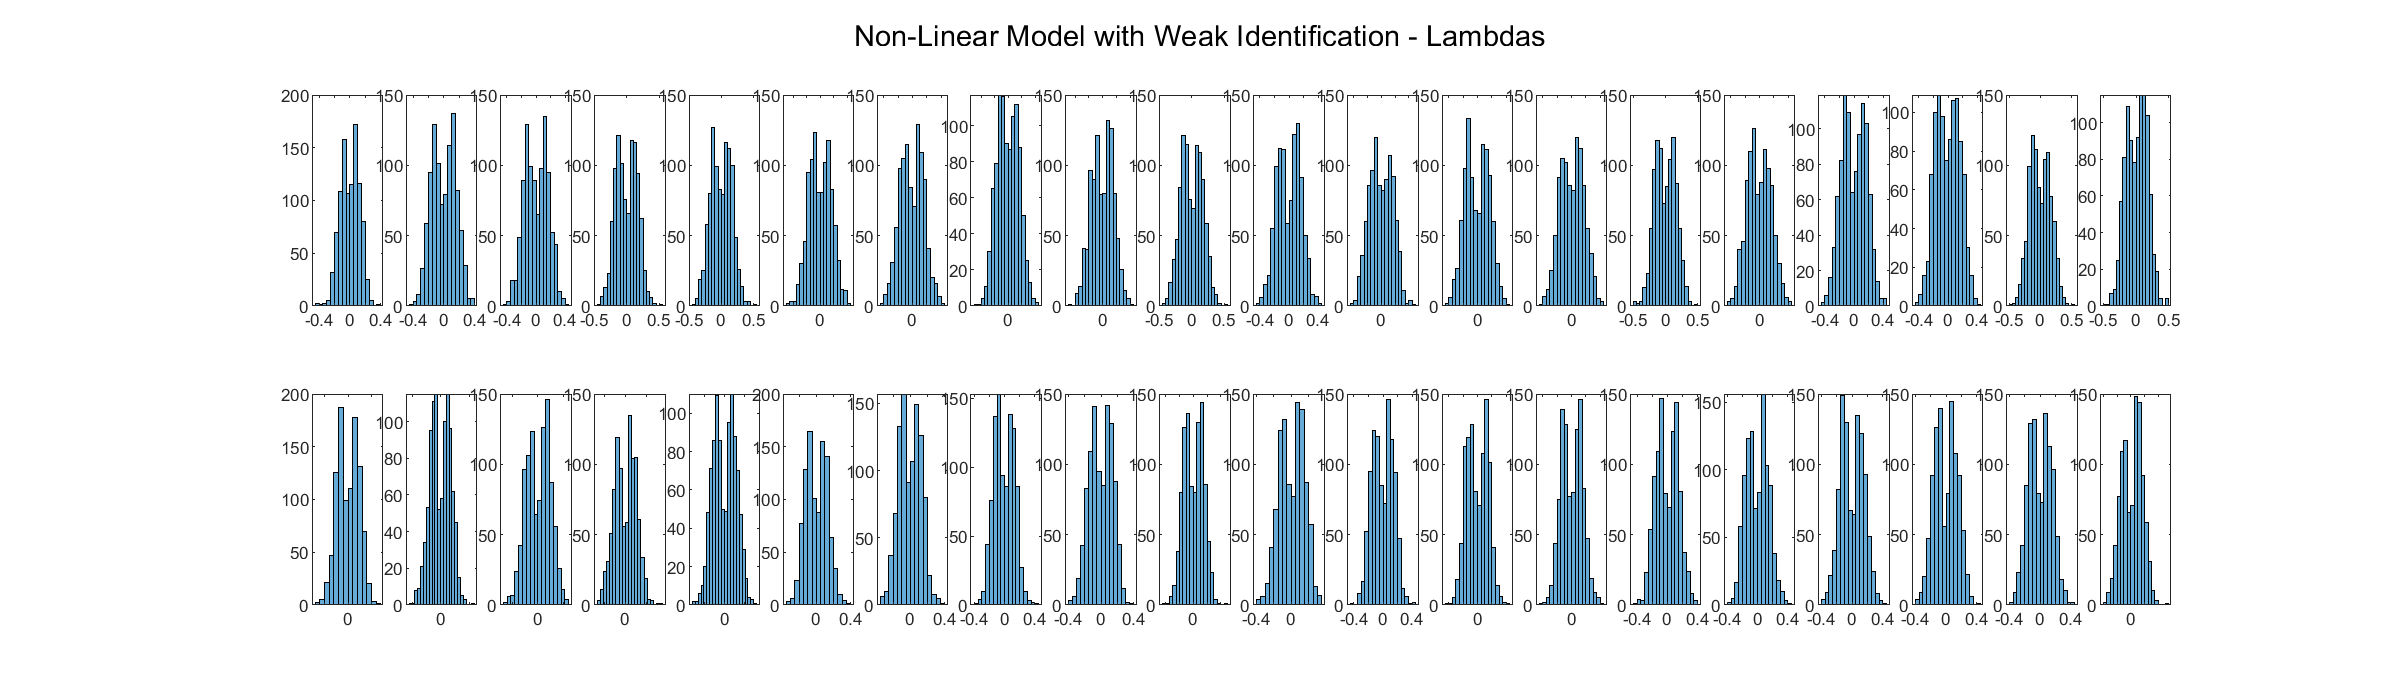
\includegraphics[scale=.3]{./tables/nonlinear_lambdas_J1000_n200_kl20.png}

{\small 
1) The non-standard distributions and 2) combining many of these distributions both affect our test statistics (blue: `standard', orange: empirical):
}

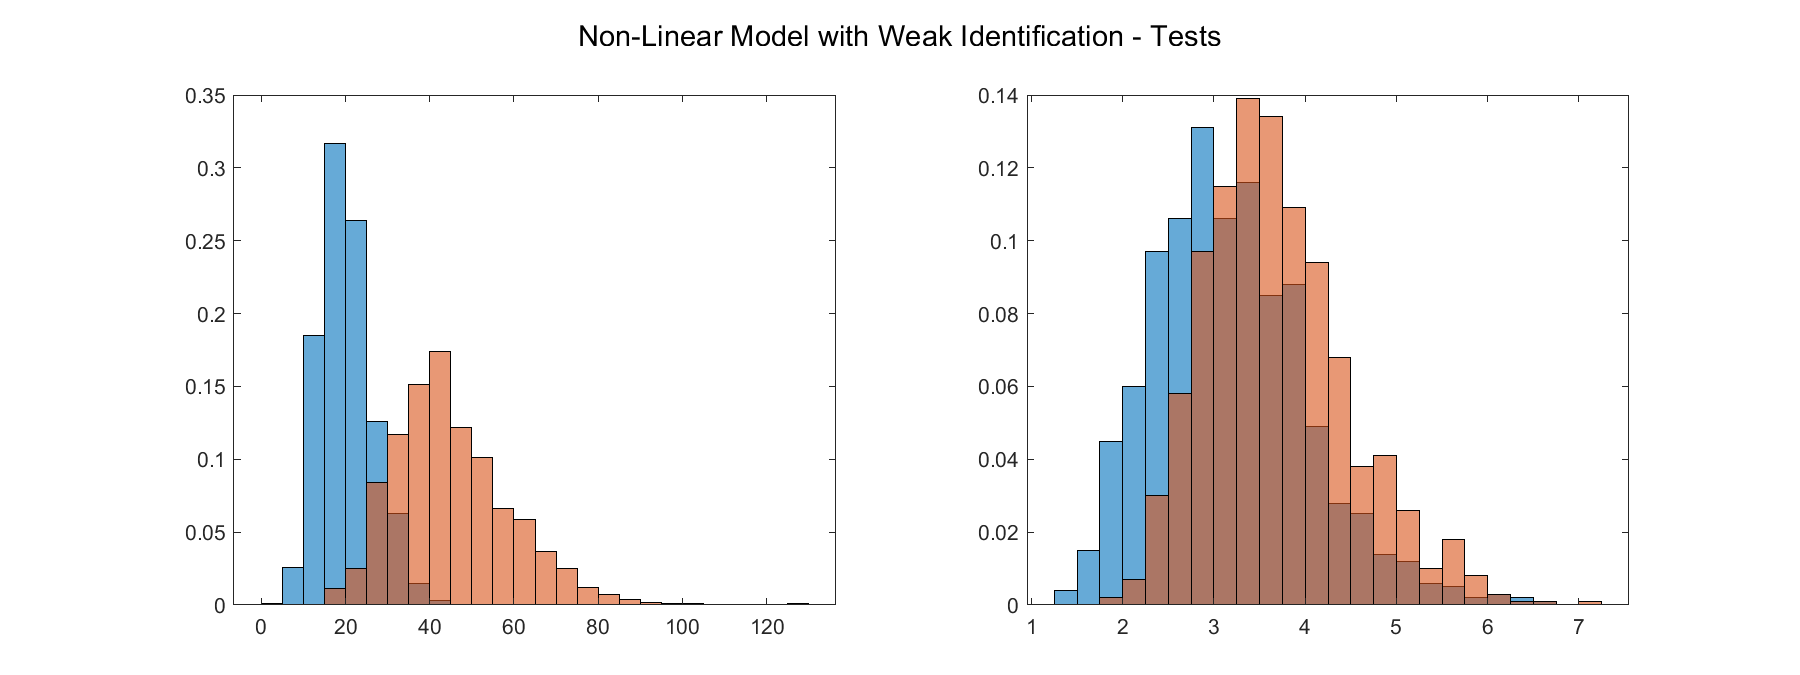
\includegraphics[scale=.25]{./tables/nonlinear_tests_J1000_n200_kl20.png}
\end{center}

\vfill
\hfill 
% \hyperlink{intro_issue2_id_failure}{\beamergotobutton{Return to Intro}}
}













\section{Empirical Example}

\addtocounter{framenumber}{-1}
\frame{
\frametitle{Outline}
\tableofcontents[ 
	currentsection, 
    %currentsubsection, 
    hideothersubsections, 
    %sectionstyle=show/hide, 
    %subsectionstyle=show/shaded, 
    ] 
}





\frame{
\frametitle{Empirical Example - Exchange Rate Modeling}
\begin{itemize}
\item Studies of PPP $\Rightarrow$ exchange rate adjustments resemble a unit root process within a band and a stationary process outside of that band. \citep{Taylor_etal2001_exchangerates_and_PPP,ObstfeldTaylor1997}

\item Large literature following \cite{Taylor_etal2001_exchangerates_and_PPP} allow a smooth transition at the boundary of the band with a `Smooth Transition Regression' Model
% \begin{equation*}
% q_{t} = \sum_{j=1}^{p} \beta_j q_{t-j} + \sum_{j=1}^{p} \beta_j^* q_{t-j} h(\gamma; q_{t-d}) + \e_t
% \end{equation*}

\item Example: \cite{Kilic2016} examines the first differenced model
\begin{align*}
\Delta q_{t} = \Big[\delta_{0} + \sum_{j=1}^{p} \delta_{j} \Delta q_{t-j} \Big] h(\gamma_{d}, \Delta q_{t-\highlight{d}}) + u_{t}
\end{align*}
where $h$ is the exponential transition function
\begin{align*}
h(\gamma; x) = 1 - \exp(-\gamma x^2 ).
\end{align*}
$q_t$ is the demeaned log real exchange rate, and $u_{t} \sim iid (0, \sigma^2)$
\end{itemize}
}








\frame{
\frametitle{Empirical Example - Exchange Rate Modeling}
% Similarly, \cite{Kilic2016} examines the first differenced model
\begin{align*}
\Delta q_{t} &= \Big[\delta_{0} + \sum_{j=1}^{p} \delta_{j} \Delta q_{t-j} \Big] h(\gamma_{d}, \Delta q_{t-\highlight{d}}) + u_{t} \\
& h(\gamma; x) = 1 - \exp(-\gamma x^2 ).
\end{align*}

\vspace*{1cm}
Two issues:
\begin{itemize}
\item The unknown value of $d$ must be selected 
\begin{itemize}
\item (a large number of lags are available).  
\end{itemize}
\item Parameter identification failure occurs when $\gamma_{d}=0$. 
\end{itemize}
}





\frame{
\frametitle{Empirical Example - Exchange Rate Modeling}
In principle, the $\delta$'s can differ by $d$
\begin{align*}
\Delta q_{t} = \Big[\delta_{\highlight{d},0} + \sum_{j=1}^{p} \delta_{\highlight{d},j} \Delta q_{t-j} \Big] h(\gamma_{\highlight{d}}, \Delta q_{t-\highlight{d}}) + u_{\highlight{d}, t}
\end{align*}
and there is an implied `belief' that $\gamma_{\tilde{d}}=0$ for any $\tilde{d} \ne d$.

This structure implies a full model:
\begin{align*}
\Delta q_{t} = \sum_{d=1}^{k} \Bigg( \Big[\delta_{\highlight{d},0} + \sum_{j=1}^{p} \delta_{\highlight{d},j} \Delta q_{t-j} \Big] h(\gamma_{\highlight{d}}, \Delta q_{t-\highlight{d}}) \Bigg) + \e_{t}
\end{align*}
where we can formulate a null hypothesis that gives the appropriate restriction on this full model.
\begin{align*}
H_{0}: \gamma_{\tilde{d}} = 0 \qquad \forall \tilde{d} \ne d
\end{align*}
}

%







\frame[label = exchange_rate_pars_models_1]{
\frametitle{Empirical Example - Exchange Rate Modeling}
This is the null for tests of no (omitted) nonlinearity.  In general, 
\begin{align*}
H_{0}: \lambda = 0_{k}
\end{align*}
where $\lambda$ is a sub-vector of $\gamma = (\gamma_{1}, \dots, \gamma_{d}, \dots)$.

\begin{itemize}
\item How do we use the max test?
\item Conveniently, the parsimonious models are already given. \\ e.g. when $\lambda = \gamma$:
\begin{align*}
\Delta q_{t} = \Big[\delta_{\highlight{d},0} + \sum_{j=1}^{p} \delta_{\highlight{d},j} \Delta q_{t-j} \Big] h(\lambda_{\highlight{d}}, \Delta q_{t-\highlight{d}}) + u_{\highlight{d}, t}
\end{align*}
% \begin{align*}
% \Delta q_{t} = \sum_{i=0}^{p} \beta_{(d),i}^{*} g_{i}(\gamma_{d}, \Delta q_{t-d}) + u_{d,t}
% \end{align*}
\begin{itemize}
\item for each $d = 1, \dots, k$
\hfill 
\hyperlink{exchange_rate_pars_models_2}{\beamergotobutton{When $\lambda$ is a sub-vector}}
% \item where $g_{i}(\gamma_{d}, \Delta q_{t-d}) = \Delta q_{t-i} h(\gamma_{d}, \Delta q_{t-d})$ for $i = 1, \dots, p$ 
% \item and $g_{0}(\gamma_{d}, \Delta q_{t-d}) = h(\gamma_{d}, \Delta q_{t-d})$.
\end{itemize}
\item Observe that $H_{0}$ $\Rightarrow$ $u_{d,t} = \e_{t}$ for every $d$
\end{itemize}
}



%



\frame{
\frametitle{Empirical Example - Exchange Rate Modeling}
\begin{itemize}
\item let $\lambda = \gamma$, 
\begin{align*}
F_{t}(\delta_{\highlight{d}}) = \delta_{\highlight{d},0} + \sum_{j=1}^{p} \delta_{\highlight{d},j} \Delta q_{t-j},
\end{align*}
and consider $H_{0}: \lambda = 0$:
\end{itemize}
\vspace*{1cm}
Construct the max statistic via the parsimonious models:
\begin{equation*}
\left.\begin{aligned}
\Delta q_{t} &= F_{t}(\hat{\delta}_{1}) h(\hat{\lambda}_{1}, \Delta q_{t-1}) + u_{1, t} \\
 & \hspace*{2cm} \vdots \\
\Delta q_{t} &= F_{t}(\hat{\delta}_{k}) h(\hat{\lambda}_{k}, \Delta q_{t-k}) + u_{k, t}
\end{aligned}\right\}
\hspace*{.3cm}
\Rightarrow
\hspace*{.3cm}
\left.\begin{aligned}
\hat{\lambda}_{1} \\ \vdots \\ \hat{\lambda}_{k}
\end{aligned}\right\}
\hspace*{.3cm}
\Rightarrow
\hspace*{.3cm}
\hat{\Tc} = \max_{1\le i \le k} |\Ns_{i} \hat{\lambda}_{i}|
\end{equation*}
}





%











% \frame[label = what_we_can_and_cant_test]{
% \frametitle{What we can and cannot test}
% Our procedure is valid for
% \begin{itemize}
% \item nuisance parameters % \cite{Davies1977}
% \item mixed identification strength % \cite{Cheng2015}
% \item testing weakly identified parameters % \cite{AndrewsCheng2012}
% \item models that can be estimated by M-estimators %  \cite{AndrewsCheng2013}
% \item large dimensional parameters
% \end{itemize}
% 
% \vspace*{1cm}
% Caveats:
% \begin{itemize}
% \item Model must have known parametric source of identification failure
% \item low power when the null involves weakly identified parameters
% \item parameter dimension can't be `too large'
% \item Max tests are better suited for certain types of alternatives
% \hyperlink{max_tests_explanation_slide}{\beamergotobutton{Max Tests?}}
% %\hyperlink{what_we_can_and_cant_test}{\beamergotobutton{Return to Caveats}}
% \end{itemize}
% 
% % link to slide for relationship to LASSO
% }









\section{Asymptotics}

\addtocounter{framenumber}{-1}
\frame{
\frametitle{Outline}
\tableofcontents[ 
	currentsection, 
    %currentsubsection, 
    hideothersubsections, 
    %sectionstyle=show/hide, 
    %subsectionstyle=show/shaded, 
    ] 
}




\frame{
\frametitle{Max Test - A Little Theory}
\begin{align*}
Y_t = \lambda_{1} h(X_t, \pi_{1}) + \lambda_{2} h(X_t, \pi_{2}) + \cdots + \lambda_{k} h(X_t, \pi_{k}) + \e_{t}
\end{align*}

\begin{align*}
H_{0}: \lambda = 0_{k}
\end{align*}

We estimate $k$ \textit{sub-models}
\begin{align*}
Y_t = \lambda_{i} h(X_t, \pi_{i}) + \nu_{i,t}, \hspace{1em} i = 1, \dots, k
\end{align*}

Then collect the estimators and form the max statistic
\begin{align*}
\hat{\mathcal{T}}_{n} = \max_{1 \le i \le k_{n}} | \Ns_{i} \hat{\lambda}_{i,n}|
\end{align*}
where $\Ns_{i} = \sqrt{n}$ in this example.
}


\frame{
\frametitle{Limiting Distribution}
% \begin{theorem}\label{T:Test stat limiting distribution}
\begin{enumerate}[a]
\item If there are weakly identified parameters, then
under some assumptions and $H_{0}$,
\begin{equation*}
\Big| \hat{\Ts}_{n} - \max_{1\le i \le \mathring{k}_{n}} |S_{(i), \lambda}' \mathfrak{Z}_{(i)}(\pi_{(i), l_{K}}^{*}(b, \gamma_{0}); \gamma_{0})| \Big| \toP 0
\end{equation*}
for some non-unique $\mathring{k}_{n} = o(n)$.
Pointwise, we have
\begin{align*}
\mathfrak{Z}_{(i)}(\pi_{(i), l_{K}}; \gamma_{0}) & =
\pmat{ \tau_{(i)}(\pi_{(i), l_{K}}^{*}(b, \gamma_{0})) - S_{l_{K}} b_{(i), l_{K}} \\ \pi_{(i), l_{K}}^{*}(b, \gamma_{0}) }
\end{align*}
where $S_{l_{K}}$ is the selection matrix that selects the columns corresponding to $\lambda_{(i), l_{k}}$.
\end{enumerate}
% \end{theorem}
}


\frame{
\frametitle{Limiting Distribution}
% \begin{theorem}[continued...]
\begin{enumerate}[b]
\item if no parameters are weakly identified
then under assumptions and $H_{0}$,
\begin{equation*}
\Big| \hat{\Ts}_{n} - \max_{1\le i \le \mathring{k}_{n}} |S_{(i), \lambda}' \mathfrak{Z}_{(i)}(\gamma_{0})| \Big| \toP 0
\end{equation*}
for some non-unique $\mathring{k}_{n} = o(n)$.
Pointwise, 
\begin{align*}
\mathfrak{Z}_{(i)}(\gamma_{0}) = 
H_{(i), K-1}(\gamma_{0})^{-1} \G_{(i), \theta}(\gamma_{0})
\end{align*}
where $\G_{(i), \theta}(\gamma_{0}) \sim N(0, \Omega_{(i), \theta}(\gamma_{0}))$.
\end{enumerate}
% \end{theorem}
}



\frame{
\frametitle{Limiting Distribution - Weak Identification}
\begin{itemize}
\item Key take away - two different distributions based on whether $\pi$ can be consistently estimated.  


\item Recall
\begin{align*}
Y_t = \lambda_{i} h(X_{i,t}, \pi_{i}) + \nu_{i,t}, \hspace{1em} i = 1, \dots, k
\end{align*}

\item $\lambda_{i}$ is ``large'' $\Rightarrow$ $\pi_{i}$ is (strongly) identified 
\begin{itemize}
\item $\hat{\pi}_{i}$ consistently estimates $\pi_{i}$
\end{itemize}

\item $\lambda_{i}$ is ``small'' 
\begin{itemize}
\item $\Rightarrow$ $\pi_{i}$ is weakly identified 
\item $\hat{\pi}_{i}$ can\highlight{not} consistent estimate $\pi_{i}$ (noise dominates the signal)
\item $\Rightarrow$ $\hat{\pi}_{i}$ has Nonstandard Distribution $(\pi_{i}^{\ast})$
\item This nonstandardness propogates to the other estimators! \\ $\Rightarrow$ $\hat{\lambda}_{i}$ also has a Nonstandard Distribution!
\end{itemize}

\end{itemize}

}





\frame[label=histogram_id_failure_single]{
\frametitle{Identification Failure: Non-Standard Distribution}
\begin{center}
\hspace{-1cm}
\includegraphics[scale=.17]{./fig/STAR_beta_hat_id1_J10000.png}
%
\hspace{-1.1cm}
\includegraphics[scale=.17]{./fig/STAR_beta_hat_id2_J10000.png}
\end{center}
\begin{align*}
Y_t = \lambda h(X_t, \pi) + \e_{t}
\end{align*}
\vfill
\hfill 
\hyperlink{intro_issue2_id_failure}{\beamergotobutton{Return to Intro}}
}


\frame[label=histogram_id_failure_multi]{ 
\frametitle{Identification Failure: Non-Standard Distribution}
\begin{center}
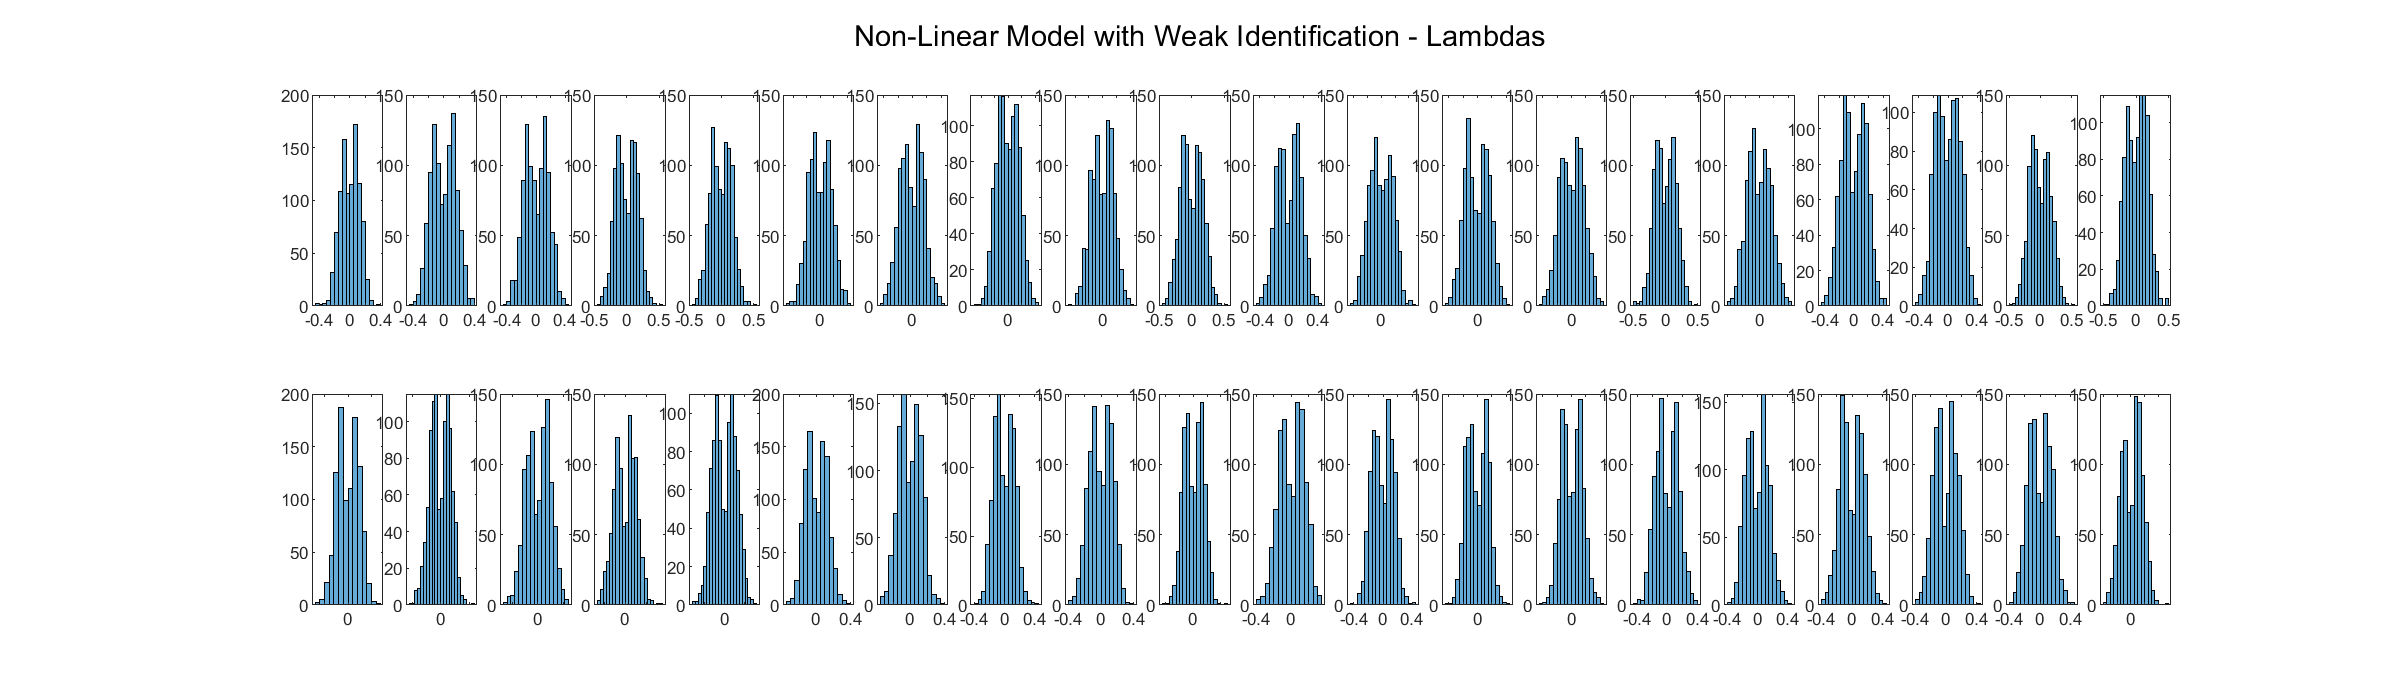
\includegraphics[scale=.3]{./tables/nonlinear_lambdas_J1000_n200_kl20.png}

{\small 
1) The non-standard distributions and 2) combining many of these distributions both affect our test statistics (blue: `standard', orange: empirical):
}

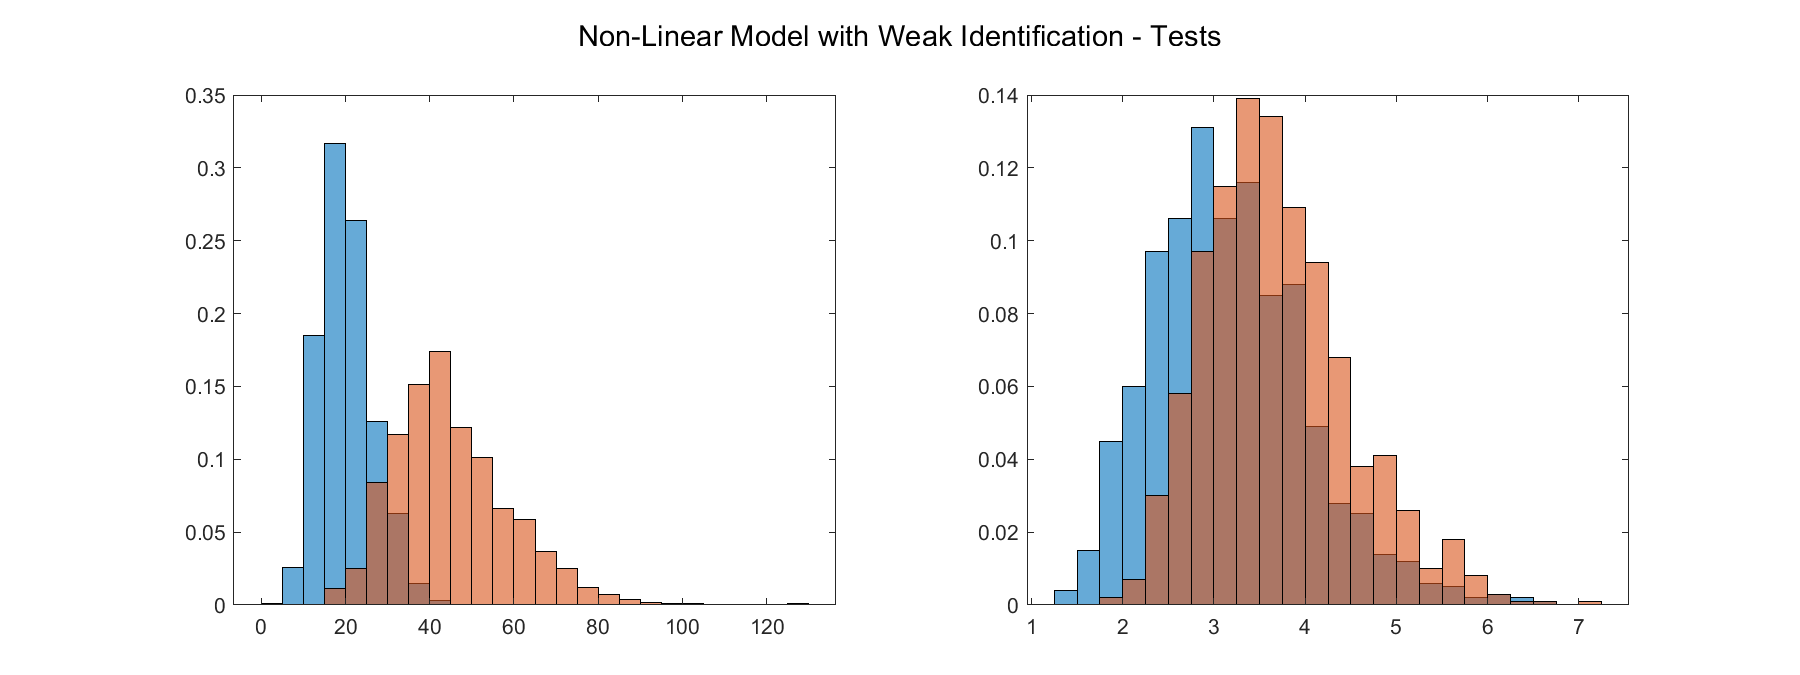
\includegraphics[scale=.25]{./tables/nonlinear_tests_J1000_n200_kl20.png}
\end{center}

\vfill
\hfill 
\hyperlink{intro_issue2_id_failure}{\beamergotobutton{Return to Intro}}
}



\frame{
\frametitle{Limiting Distribution Note on Assumptions}
\begin{itemize}
\item Needed restrictions on the functional form of the model

\vspace*{.5cm}
\item There must be a parametric source of identification failure
e.g. $y_{t} = \beta h(X_{t}, \pi) + \e_{t}$:  $\beta = 0$ $\Rightarrow$ $\pi$ is unidentified

\vspace*{.5cm}
\item There can be more than one source of identification failure, but each can only affect its own parameters e.g.
$y_{t} = \beta_{1} h(X_{1,t}, \pi_{1}) + \beta_{2} h(X_{2,t}, \pi_{2}) + \e_{t}$

\vspace*{.5cm}
\item The derivatives of the criterion functions agree for the full and sub models
\end{itemize}
}






\section{Inference}

\addtocounter{framenumber}{-1}
\frame{
\frametitle{Outline}
\tableofcontents[ 
	currentsection, 
    %currentsubsection, 
    hideothersubsections, 
    %sectionstyle=show/hide, 
    %subsectionstyle=show/shaded, 
    ] 
}








\frame[label = bootstrapping_the_max_test_is_new]{
\frametitle{Inference}
\begin{itemize}
\item Inference usually relies on calculation of asymptotic distribution. \citep{deHaan1976}
\item But EVT requires conditions that might be too restrictive \citep{HillMontegi2016_many_zeros,HillMontegi2016_white_noise} 
\begin{itemize}
\item (e.g. dependence properties, non-standard distributions)
\end{itemize}
\item Instead, we provide a bootstrap procedure to simulate the distribution


\vspace*{.5cm}
\item Bootstrapping this type of test is new \citep{Chernozhukov_etal2013,Chernozhukov_etal2016,ZhangCheng2017,ZhangWu2017,HillMontegi2016_white_noise,HillMontegi2016_many_zeros}

We must account for 
\begin{itemize}
\item Dependence in the estimators (e.g. omitted variable bias)
\item Non-standard distributions (identification failure)
\end{itemize}
\end{itemize}

\vfill
\hfill 
% \hyperlink{critical_values_short_slide}{\beamergotobutton{Return to Inference Procedure}}
% \hyperlink{bootstrapping_the_max_test_is_new}{\beamergotobutton{Bootstrapping a Max Test?}}
}









\frame[label = critical_values_short_slide]{
\frametitle{Inference}
% \begin{itemize}
% \item Inference on a maximum usually relies on calculated asymptotic distribution
% \item But we can't do that here
% \item Instead, we provide a bootstrap procedure to simulate the distribution
% \hyperlink{bootstrapping_the_max_test_is_new}{\beamergotobutton{Bootstrapping a Max Statistic?}}
% \end{itemize}


\vspace*{1cm}
Recall 2 distributions 
% \hyperlink{Test_stat_theorem}{\beamergotobutton{Theory}}

\begin{itemize}
\item We don't know which is correct - must bootstrap each individually
% \hyperlink{bootstrap_procedure}{\beamergotobutton{ Bootstrap Procedure}}

\item 2 different critical values - How to combine them?

\item ICS - Use data to determine if parameter is identified
\hyperlink{robust_cvs}{\beamergotobutton{ICS Details}}

\begin{itemize}
\item if so, then use identified cv
\item if not, take the larger of the 2 cvs
\end{itemize}
\end{itemize}
}





\frame[label = Inference_Procedure_sim]{
\frametitle{Inference Procedure}
Gaussian Multiplier Bootstrap:
\begin{enumerate}
\item 
First, draw a Gaussian multiplier sequence $Z_t$

\item 
For each Parsimonious Model:
\begin{enumerate}[a]
\item 
Use ICS pretest to determine which parameters are strongly identified.  
Place the remainder in group $l_K$.

\item 
Use $Z_t$ to form key quantities $\mathfrak{Z}_{i}(\pi_{i, l_{K}}; \gamma_{0})$ and $\pi_{i, l_{K}}^{\ast}(b, \gamma_{0})$.
\hfill \hyperlink{Inference_sim_step_2b}{\beamergotobutton{ Inference Step 2b}}

\item 
Collect the resulting values corresponding to $\lambda$, and use them to form the test statistic.
\end{enumerate}

\item 
Repeat above steps $M$ times

\item 
Form $\alpha$-level critical values, $cv(b, \gamma_{0})$.

\item Repeat on a grid of the nuisance parameters, and take the largest of the critical values.
\end{enumerate}
% \hfill \hyperlink{Inference_Procedure_sim}{\beamergotobutton{ Inference Procedure}}
}











\section{Simulation}

\addtocounter{framenumber}{-1}
\frame{
\frametitle{Outline}
\tableofcontents[ 
	currentsection, 
    %currentsubsection, 
    hideothersubsections, 
    %sectionstyle=show/hide, 
    %subsectionstyle=show/shaded, 
    ] 
}



\frame{
\frametitle{Simulation Setup}
Consider the additive non-linear model
\begin{align*}
Y_t = \zeta + \beta_{1} h(\tilde{X}_{1,t}, \tilde{\pi}_{1}) + \lambda_{1} h(X_{1,t}, \pi_{1}) + \cdots + \lambda_{k} h(X_{k,t}, \pi_{k}) + \e_{t}
\end{align*}
% \begin{align*}
% Y_{t} = \zeta + \sum_{j=1}^{d_{\beta}} \beta_{j} h_{j}(X_{j,t}, \pi_{j}) + \e_{t}
% \end{align*}
with 
\begin{equation*}
h_{j}(X_{j,t}, \pi_{j}) = X_{j,t}\Big[ 1 - \exp(-c (Z_{t} - \pi_{j})^2 ) \Big],
\end{equation*}

\begin{itemize}
\item 
Correlated Regressors:  $X_{t} \sim N(0_{d_{\beta}}, \Sigma_{x})$,  $\e_{t}$ $\sim$ iid $N(0,1)$.

\item
Set $c = 10$ for convenience, 

\item 
Consider $\beta_{1} \in \{0, 1/\sqrt{n}, 1\} $ 

% \item
% and $\beta_{i} = 0$ for $i>1$.

\item 
Test $H_{0}: \lambda_{i} = 0$ for every $i$ 
% where $\lambda_{i} = \beta_{i+1}$ for $i = 1, \dots, d_{\beta}-1$.
\end{itemize}
}










\frame[label = simulation_results_null_table]{
\frametitle{Simulation Results}
 \begin{table}[H] 
 \singlespacing 
 \small 
 \centering 
\begin{tabular}{c|ccc|ccc} 
\multicolumn{7}{c}{ Rejection Frequencies, Experiment: 1, DGP: 2, Hyp: Null } \\ 
\multicolumn{7}{c}{ $H_0: \highlight{\lambda_{i} = 0} \quad i = 1,\dots,d_{\beta}-1$} \\
\multicolumn{7}{c}{ $n=200$, $J=10000$, $\alpha = 0.05$ } \\ 
 \multicolumn{1}{c}{} & \multicolumn{3}{c}{ $k_{\lambda,n}=1$ } & \multicolumn{3}{c}{ $k_{\lambda,n}=20$ } \\ 
 \hline 
 $\beta_{1}$ & $0$ & $1/\sqrt{n}$  & $1$ & $0$ & $1/\sqrt{n}$  & $1$   \\ 
 \hline 
 \hline 
 Wald Test Standard &  0.11 &  0.12  &  \highlight{0.12} &  0.83 &  0.84  &  0.84 \\ 
 Max Test Standard &  0.10 &  0.10  &  \highlight{0.10} &  0.12 &  0.11  &  0.11 \\ 
 Max t-Test Standard &  0.11 &  0.12  &  \highlight{0.11} &  0.19 &  0.19  &  0.20 \\ 
 \hline 
 Wald Test BS1 &  0.06 &  0.06  &  0.06 &  0.68 &  0.68  &  0.69 \\ 
 Max Test BS1 &  0.04 &  0.04  &  0.04 &  0.03 &  0.03  &  0.03 \\ 
 Max t-Test BS1 &  0.06 &  0.06  &  0.06 &  0.13 &  0.12  &  0.13 \\ 
 \hline 
 Wald Test BS2 &  0.06 &  0.06  &  0.06 &  0.25 &  0.26  &  0.25 \\ 
 Max Test BS2 &  0.05 &  0.05  &  0.05 &  0.04 &  0.04  &  0.04 \\ 
 Max t-Test BS2 &  0.06 &  0.06  &  0.06 &  0.08 &  0.08  &  0.09 \\ 
 \hline 
% Wald Test Taylor &  0.09 &  0.09  &  0.09 &  0.52 &  0.52  &  0.52 \\ 
% Max Test Taylor &  0.60 &  0.60  &  0.60 &  0.99 &  0.99  &  0.99 \\ 
% Max t-Test Taylor &  0.09 &  0.09  &  0.09 &  0.16 &  0.16  &  0.16 \\ 
% \hline 
\end{tabular}
 \end{table}

\hfill 
\hyperlink{simulation_results_null_histograms}{\beamergotobutton{Histograms}}
\hyperlink{simulation_results_null_table_full}{\beamergotobutton{Full table}}
}


\addtocounter{framenumber}{-1}
\frame[label = simulation_results_null_table]{
\frametitle{Simulation Results}
 \begin{table}[H] 
 \singlespacing 
 \small 
 \centering 
\begin{tabular}{c|ccc|ccc} 
\multicolumn{7}{c}{ Rejection Frequencies, Experiment: 1, DGP: 2, Hyp: Null } \\ 
\multicolumn{7}{c}{ $H_0: \highlight{\lambda_{i} = 0} \quad i = 1,\dots,d_{\beta}-1$} \\
\multicolumn{7}{c}{ $n=200$, $J=10000$, $\alpha = 0.05$ } \\ 
 \multicolumn{1}{c}{} & \multicolumn{3}{c}{ $k_{\lambda,n}=1$ } & \multicolumn{3}{c}{ $k_{\lambda,n}=20$ } \\ 
 \hline 
 $\beta_{1}$ & $0$ & $1/\sqrt{n}$  & $1$ & $0$ & $1/\sqrt{n}$  & $1$   \\ 
 \hline 
 \hline 
 Wald Test Standard &  0.11 &  0.12  &  0.12 &  0.83 &  0.84  &  0.84 \\ 
 Max Test Standard &  0.10 &  0.10  &  0.10 &  0.12 &  0.11  &  0.11 \\ 
 Max t-Test Standard &  0.11 &  0.12  &  0.11 &  0.19 &  0.19  &  0.20 \\ 
 \hline 
 Wald Test BS1 &  0.06 &  0.06  &  \highlight{0.06} &  0.68 &  0.68  &  0.69 \\ 
 Max Test BS1 &  0.04 &  0.04  &  \highlight{0.04} &  0.03 &  0.03  &  0.03 \\ 
 Max t-Test BS1 &  0.06 &  0.06  &  \highlight{0.06} &  0.13 &  0.12  &  0.13 \\ 
 \hline 
 Wald Test BS2 &  0.06 &  0.06  &  0.06 &  0.25 &  0.26  &  0.25 \\ 
 Max Test BS2 &  0.05 &  0.05  &  0.05 &  0.04 &  0.04  &  0.04 \\ 
 Max t-Test BS2 &  0.06 &  0.06  &  0.06 &  0.08 &  0.08  &  0.09 \\ 
 \hline 
% Wald Test Taylor &  0.09 &  0.09  &  0.09 &  0.52 &  0.52  &  0.52 \\ 
% Max Test Taylor &  0.60 &  0.60  &  0.60 &  0.99 &  0.99  &  0.99 \\ 
% Max t-Test Taylor &  0.09 &  0.09  &  0.09 &  0.16 &  0.16  &  0.16 \\ 
% \hline 
\end{tabular}
 \end{table}

\hfill 
\hyperlink{simulation_results_null_histograms}{\beamergotobutton{Histograms}}
\hyperlink{simulation_results_null_table_full}{\beamergotobutton{Full table}}
}


\addtocounter{framenumber}{-1}
\frame[label = simulation_results_null_table]{
\frametitle{Simulation Results}
 \begin{table}[H] 
 \singlespacing 
 \small 
 \centering 
\begin{tabular}{c|ccc|ccc} 
\multicolumn{7}{c}{ Rejection Frequencies, Experiment: 1, DGP: 2, Hyp: Null } \\ 
\multicolumn{7}{c}{ $H_0: \highlight{\lambda_{i} = 0} \quad i = 1,\dots,d_{\beta}-1$} \\
\multicolumn{7}{c}{ $n=200$, $J=10000$, $\alpha = 0.05$ } \\ 
 \multicolumn{1}{c}{} & \multicolumn{3}{c}{ $k_{\lambda,n}=1$ } & \multicolumn{3}{c}{ $k_{\lambda,n}=20$ } \\ 
 \hline 
 $\beta_{1}$ & $0$ & $1/\sqrt{n}$  & $1$ & $0$ & $1/\sqrt{n}$  & $1$   \\ 
 \hline 
 \hline 
 Wald Test Standard &  0.11 &  0.12  &  0.12 &  0.83 &  0.84  &  \highlight{0.84} \\ 
 Max Test Standard &  0.10 &  0.10  &  0.10 &  0.12 &  0.11  &  \highlight{0.11} \\ 
 Max t-Test Standard &  0.11 &  0.12  &  0.11 &  0.19 &  0.19  &  \highlight{0.20} \\ 
 \hline 
 Wald Test BS1 &  0.06 &  0.06  &  0.06 &  0.68 &  0.68  &  0.69 \\ 
 Max Test BS1 &  0.04 &  0.04  &  0.04 &  0.03 &  0.03  &  0.03 \\ 
 Max t-Test BS1 &  0.06 &  0.06  &  0.06 &  0.13 &  0.12  &  0.13 \\ 
 \hline 
 Wald Test BS2 &  0.06 &  0.06  &  0.06 &  0.25 &  0.26  &  0.25 \\ 
 Max Test BS2 &  0.05 &  0.05  &  0.05 &  0.04 &  0.04  &  0.04 \\ 
 Max t-Test BS2 &  0.06 &  0.06  &  0.06 &  0.08 &  0.08  &  0.09 \\ 
 \hline 
% Wald Test Taylor &  0.09 &  0.09  &  0.09 &  0.52 &  0.52  &  0.52 \\ 
% Max Test Taylor &  0.60 &  0.60  &  0.60 &  0.99 &  0.99  &  0.99 \\ 
% Max t-Test Taylor &  0.09 &  0.09  &  0.09 &  0.16 &  0.16  &  0.16 \\ 
% \hline 
\end{tabular}
 \end{table}

\hfill 
\hyperlink{simulation_results_null_histograms}{\beamergotobutton{Histograms}}
\hyperlink{simulation_results_null_table_full}{\beamergotobutton{Full table}}
}



\addtocounter{framenumber}{-1}
\frame[label = simulation_results_null_table]{
\frametitle{Simulation Results}
 \begin{table}[H] 
 \singlespacing 
 \small 
 \centering 
\begin{tabular}{c|ccc|ccc} 
\multicolumn{7}{c}{ Rejection Frequencies, Experiment: 1, DGP: 2, Hyp: Null } \\ 
\multicolumn{7}{c}{ $H_0: \highlight{\lambda_{i} = 0} \quad i = 1,\dots,d_{\beta}-1$} \\
\multicolumn{7}{c}{ $n=200$, $J=10000$, $\alpha = 0.05$ } \\ 
 \multicolumn{1}{c}{} & \multicolumn{3}{c}{ $k_{\lambda,n}=1$ } & \multicolumn{3}{c}{ $k_{\lambda,n}=20$ } \\ 
 \hline 
 $\beta_{1}$ & $0$ & $1/\sqrt{n}$  & $1$ & $0$ & $1/\sqrt{n}$  & $1$   \\ 
 \hline 
 \hline 
 Wald Test Standard &  0.11 &  0.12  &  0.12 &  0.83 &  0.84  &  0.84 \\ 
 Max Test Standard &  0.10 &  0.10  &  0.10 &  0.12 &  0.11  &  0.11 \\ 
 Max t-Test Standard &  0.11 &  0.12  &  0.11 &  0.19 &  0.19  &  0.20 \\ 
 \hline 
 Wald Test BS1 &  0.06 &  0.06  &  0.06 &  0.68 &  0.68  &  \highlight{0.69} \\ 
 Max Test BS1 &  0.04 &  0.04  &  0.04 &  0.03 &  0.03  &  \highlight{0.03} \\ 
 Max t-Test BS1 &  0.06 &  0.06  &  0.06 &  0.13 &  0.12  &  \highlight{0.13} \\ 
 \hline 
 Wald Test BS2 &  0.06 &  0.06  &  0.06 &  0.25 &  0.26  &  0.25 \\ 
 Max Test BS2 &  0.05 &  0.05  &  0.05 &  0.04 &  0.04  &  0.04 \\ 
 Max t-Test BS2 &  0.06 &  0.06  &  0.06 &  0.08 &  0.08  &  0.09 \\ 
 \hline 
% Wald Test Taylor &  0.09 &  0.09  &  0.09 &  0.52 &  0.52  &  0.52 \\ 
% Max Test Taylor &  0.60 &  0.60  &  0.60 &  0.99 &  0.99  &  0.99 \\ 
% Max t-Test Taylor &  0.09 &  0.09  &  0.09 &  0.16 &  0.16  &  0.16 \\ 
% \hline 
\end{tabular}
 \end{table}

\hfill 
\hyperlink{simulation_results_null_histograms}{\beamergotobutton{Histograms}}
\hyperlink{simulation_results_null_table_full}{\beamergotobutton{Full table}}
}




%



\frame{
\frametitle{Simulation Results}
 \begin{table}[H] 
 \singlespacing 
 \small 
 \centering 
\begin{tabular}{c|ccc|ccc} 
\multicolumn{7}{c}{ Rejection Frequencies, Experiment: 1, DGP: 2, Hyp: Local Alternative } \\ 
\multicolumn{7}{c}{ $H_{LA}: \highlight{\lambda_{1} = 1/\sqrt{n}}, \ \lambda_{i} = 0 \ \forall i\ge 2$ } \\
\multicolumn{7}{c}{ $n=200$, $J=10000$, $\alpha = 0.05$ } \\ 
  \multicolumn{1}{c}{} & \multicolumn{3}{c}{ $k_{\lambda,n}=1$ } & \multicolumn{3}{c}{ $k_{\lambda,n}=20$ } \\ 
 \hline 
 $\beta_{1}$ & $0$ & $1/\sqrt{n}$  & $1$ & $0$ & $1/\sqrt{n}$  & $1$   \\ 
 \hline 
 \hline 
 Wald Test Standard &  0.21 &  0.22  &  \highlight{0.21} &  0.91 &  0.91  &  0.91 \\ 
 Max Test Standard &  0.19 &  0.20  &   \highlight{0.19} &  0.25 &  0.25  &  0.25 \\ 
 Max t-Test Standard &  0.20 &  0.20  &   \highlight{0.21} &  0.50 &  0.50  &  0.50 \\ 
 \hline 
 Wald Test BS1 &  0.12 &  0.12  &   \highlight{0.12} &  0.81 &  0.80  &  0.80 \\ 
 Max Test BS1 &  0.09 &  0.09  &   \highlight{0.09} &  0.09 &  0.09  &  0.10 \\ 
 Max t-Test BS1 &  0.12 &  0.12  &   \highlight{0.12} &  0.42 &  0.42  &  0.43 \\ 
 \hline 
 Wald Test BS2 &  0.13 &  0.13  &  0.13 &  0.39 &  0.39  &  0.39 \\ 
 Max Test BS2 &  0.11 &  0.11  &  0.11 &  0.11 &  0.10  &  0.11 \\ 
 Max t-Test BS2 &  0.13 &  0.13  &  0.13 &  0.34 &  0.33  &  0.33 \\ 
 \hline 
% Wald Test Taylor &  0.15 &  0.15  &  0.15 &  0.61 &  0.61  &  0.61 \\ 
% Max Test Taylor &  0.71 &  0.71  &  0.71 &  1.00 &  1.00  &  1.00 \\ 
% Max t-Test Taylor &  0.15 &  0.15  &  0.15 &  0.37 &  0.37  &  0.37 \\ 
% \hline 
\end{tabular}
 \end{table}

}

\addtocounter{framenumber}{-1}
\frame{
\frametitle{Simulation Results}
 \begin{table}[H] 
 \singlespacing 
 \small 
 \centering 
\begin{tabular}{c|ccc|ccc} 
\multicolumn{7}{c}{ Rejection Frequencies, Experiment: 1, DGP: 2, Hyp: Local Alternative } \\ 
\multicolumn{7}{c}{ $H_{LA}: \highlight{\lambda_{1} = 1/\sqrt{n}}, \ \lambda_{i} = 0 \ \forall i\ge 2$ } \\
\multicolumn{7}{c}{ $n=200$, $J=10000$, $\alpha = 0.05$ } \\ 
  \multicolumn{1}{c}{} & \multicolumn{3}{c}{ $k_{\lambda,n}=1$ } & \multicolumn{3}{c}{ $k_{\lambda,n}=20$ } \\ 
 \hline 
 $\beta_{1}$ & $0$ & $1/\sqrt{n}$  & $1$ & $0$ & $1/\sqrt{n}$  & $1$   \\ 
 \hline 
 \hline 
 Wald Test Standard &  0.21 &  0.22  &  0.21 &  0.91 &  0.91  &   \highlight{0.91} \\ 
 Max Test Standard &  0.19 &  0.20  &  0.19 &  0.25 &  0.25  &   \highlight{0.25} \\ 
 Max t-Test Standard &  0.20 &  0.20  &  0.21 &  0.50 &  0.50  &   \highlight{0.50} \\ 
 \hline 
 Wald Test BS1 &  0.12 &  0.12  &  0.12 &  0.81 &  0.80  &  0.80 \\ 
 Max Test BS1 &  0.09 &  0.09  &  0.09 &  0.09 &  0.09  &  0.10 \\ 
 Max t-Test BS1 &  0.12 &  0.12  &  0.12 &  0.42 &  0.42  &  0.43 \\ 
 \hline 
 Wald Test BS2 &  0.13 &  0.13  &  0.13 &  0.39 &  0.39  &  0.39 \\ 
 Max Test BS2 &  0.11 &  0.11  &  0.11 &  0.11 &  0.10  &  0.11 \\ 
 Max t-Test BS2 &  0.13 &  0.13  &  0.13 &  0.34 &  0.33  &  0.33 \\ 
 \hline 
% Wald Test Taylor &  0.15 &  0.15  &  0.15 &  0.61 &  0.61  &  0.61 \\ 
% Max Test Taylor &  0.71 &  0.71  &  0.71 &  1.00 &  1.00  &  1.00 \\ 
% Max t-Test Taylor &  0.15 &  0.15  &  0.15 &  0.37 &  0.37  &  0.37 \\ 
% \hline 
\end{tabular}
 \end{table}

}

\addtocounter{framenumber}{-1}
\frame{
\frametitle{Simulation Results}
 \begin{table}[H] 
 \singlespacing 
 \small 
 \centering 
\begin{tabular}{c|ccc|ccc} 
\multicolumn{7}{c}{ Rejection Frequencies, Experiment: 1, DGP: 2, Hyp: Local Alternative } \\ 
\multicolumn{7}{c}{ $H_{LA}: \highlight{\lambda_{1} = 1/\sqrt{n}}, \ \lambda_{i} = 0 \ \forall i\ge 2$ } \\
\multicolumn{7}{c}{ $n=200$, $J=10000$, $\alpha = 0.05$ } \\ 
  \multicolumn{1}{c}{} & \multicolumn{3}{c}{ $k_{\lambda,n}=1$ } & \multicolumn{3}{c}{ $k_{\lambda,n}=20$ } \\ 
 \hline 
 $\beta_{1}$ & $0$ & $1/\sqrt{n}$  & $1$ & $0$ & $1/\sqrt{n}$  & $1$   \\ 
 \hline 
 \hline 
 Wald Test Standard &  0.21 &  0.22  &  0.21 &  0.91 &  0.91  &  0.91 \\ 
 Max Test Standard &  0.19 &  0.20  &  0.19 &  0.25 &  0.25  &  0.25 \\ 
 Max t-Test Standard &  0.20 &  0.20  &  0.21 &  0.50 &  0.50  &  0.50 \\ 
 \hline 
 Wald Test BS1 &  0.12 &  0.12  &  0.12 &  0.81 &  0.80  &   \highlight{0.80} \\ 
 Max Test BS1 &  0.09 &  0.09  &  0.09 &  0.09 &  0.09  &   \highlight{0.10} \\ 
 Max t-Test BS1 &  0.12 &  0.12  &  0.12 &  0.42 &  0.42  &   \highlight{0.43} \\ 
 \hline 
 Wald Test BS2 &  0.13 &  0.13  &  0.13 &  0.39 &  0.39  &  0.39 \\ 
 Max Test BS2 &  0.11 &  0.11  &  0.11 &  0.11 &  0.10  &  0.11 \\ 
 Max t-Test BS2 &  0.13 &  0.13  &  0.13 &  0.34 &  0.33  &  0.33 \\ 
 \hline 
% Wald Test Taylor &  0.15 &  0.15  &  0.15 &  0.61 &  0.61  &  0.61 \\ 
% Max Test Taylor &  0.71 &  0.71  &  0.71 &  1.00 &  1.00  &  1.00 \\ 
% Max t-Test Taylor &  0.15 &  0.15  &  0.15 &  0.37 &  0.37  &  0.37 \\ 
% \hline 
\end{tabular}
 \end{table}

}





\frame{
\frametitle{Simulation Results}
 \begin{table}[H] 
 \singlespacing 
 \small 
 \centering 
\begin{tabular}{c|ccc|ccc} 
\multicolumn{7}{c}{ Rejection Frequencies, Experiment: 1, DGP: 2, Hyp: Alternative } \\ 
\multicolumn{7}{c}{ $H_{A}: \highlight{\lambda_{1} = 1}, \lambda_{i} = 0 \ \forall i\ge 2$ } \\
\multicolumn{7}{c}{ $n=200$, $J=10000$, $\alpha = 0.05$ } \\ 
  \multicolumn{1}{c}{} & \multicolumn{3}{c}{ $k_{\lambda,n}=1$ } & \multicolumn{3}{c}{ $k_{\lambda,n}=20$ } \\ 
 \hline 
 $\beta_{1}$ & $0$ & $1/\sqrt{n}$ &  $1$ & $0$ & $1/\sqrt{n}$  & $1$   \\ 
 \hline  
 \hline 
 Wald Test Standard  &  1.00 &  1.00 &  1.00 &  1.00 &  1.00 &  1.00 \\ 
 Max Test Standard &  1.00 &  1.00 &  1.00 &  1.00 &  1.00 &  1.00  \\ 
 Max t-Test Standard &  1.00 &  1.00 &  1.00 &  1.00 &  1.00 &  1.00  \\ 
 \hline  
 Wald Test BS1 &  1.00 &  1.00 &  1.00 &  1.00 &  1.00 &  1.00  \\ 
 Max Test BS1 &  1.00 &  1.00 &  1.00 &  1.00 &  1.00 &  1.00  \\ 
 Max t-Test BS1 &  1.00 &  1.00 &  1.00 &  1.00 &  1.00 &  1.00  \\ 
 \hline  
 Wald Test BS2 &  1.00 &  1.00 &  1.00 &  1.00 &  1.00 &  1.00  \\ 
 Max Test BS2 &  1.00 &  1.00 &  1.00 &  1.00 &  1.00 &  1.00  \\ 
 Max t-Test BS2 &  1.00 &  1.00 &  1.00 &  1.00 &  1.00 &  1.00  \\ 
 \hline  
% Wald Test Taylor &  1.00 &  1.00 &  1.00 &  1.00 &  1.00 &  1.00  \\ 
% Max Test Taylor &  1.00 &  1.00 &  1.00 &  1.00 &  1.00 &  1.00  \\ 
% Max t-Test Taylor &  1.00 &  1.00 &  1.00 &  1.00 &  1.00 &  1.00  \\ 
% \hline 
\end{tabular}
 \end{table}

}







\frame[label = conclusion]{
\frametitle{Conclusion}
\begin{itemize}
\item Traditional Inference is distorted with
\begin{itemize}
\item Large dimensional (k) parameters
\item Identification Failure
\end{itemize}

\item Previous work addresses 
\begin{itemize}
\item identification failure %\textit{for small $k$ and a specific class of models}
\item large $k$ without identification failure
\end{itemize}

\item Some economic questions require considering both

\item Our max test accommodates weak identification and large $k$ % for a broad class of models.
\end{itemize}

}





% \frame{
% Empirical Example Results
% }







%%%%%%%%%%%%%%%%%%%%%%%%
%%%%%%%%%%%%%%%%%%%%%%%%
%%%%%%%%%%%%%%%%%%%%%%%%
%%%%%%%%%%%%%%%%%%%%%%%%
%%%%%%%%%%%%%%%%%%%%%%%%
%%%%%%%%%%%%%%%%%%%%%%%%
%%%%%%%%%%%%%%%%%%%%%%%%
%%%%%%%%%%%%%%%%%%%%%%%%
%%%%%%%%%%%%%%%%%%%%%%%%
%%%%%%%%%%%%%%%%%%%%%%%%
%%%%%%%%%%%%%%%%%%%%%%%%
%%%%%%%%%%%%%%%%%%%%%%%%
%%%%%%%%%%%%%%%%%%%%%%%%
%%%%%%%%%%%%%%%%%%%%%%%%
%%%%%%%%%%%%%%%%%%%%%%%%
%%%%%%%%%%%%%%%%%%%%%%%%
%%%%%%%%%%%%%%%%%%%%%%%%
%%%%%%%%%%%%%%%%%%%%%%%%
%%%%%%%%%%%%%%%%%%%%%%%%
\beginbackup

\frame{
\begin{center}
\LARGE Thank You!
\end{center}
}










\section*{References}
% % REFERENCES
\frame[allowframebreaks]{
\frametitle{References}
\tiny
\bibliographystyle{ecta}
\bibliography{../../ref_max_test_weak_id}
}















\section*{Appendix}


\frame{
\frametitle{Appendix Slides follow}
\begin{center}
Appendix Slides follow
\end{center}
}



\subsection*{The Setup}

\frame[label = max_test_general_setup]{
\frametitle{Max Test - General Setup}
Appropriate for models estimated with M-estimators (under mixing and moment conditions):
\begin{align*}
Q_{n} = \frac{1}{n} \sum_{t=1}^{n} m_{t}(\theta)
\end{align*}

The parsimonious models are defined by
\begin{align*}
Q_{(i), n} = \frac{1}{n} \sum_{t=1}^{n} m_{(i), t}(\theta_{(i)})
\end{align*}

where
\begin{align*}
m_{(i), t}(\theta_{(i)}) = m_{t}(\underbrace{(\delta, 0, \dots, \lambda_{i}, 0, \dots, \tilde{\delta}_{i})}_{\theta_{(i)} = [\theta]_{(i)}})
\end{align*}
\vfill
\hfill 
%\hyperlink{max_test_general_setup}{\beamergotobutton{Generalized Setup}}
\hyperlink{max_test_example_setup}{\beamergotobutton{Return to Example Setup}}
}




\subsection*{Initial Histograms}
\frame{ 
\frametitle{}
\begin{center}
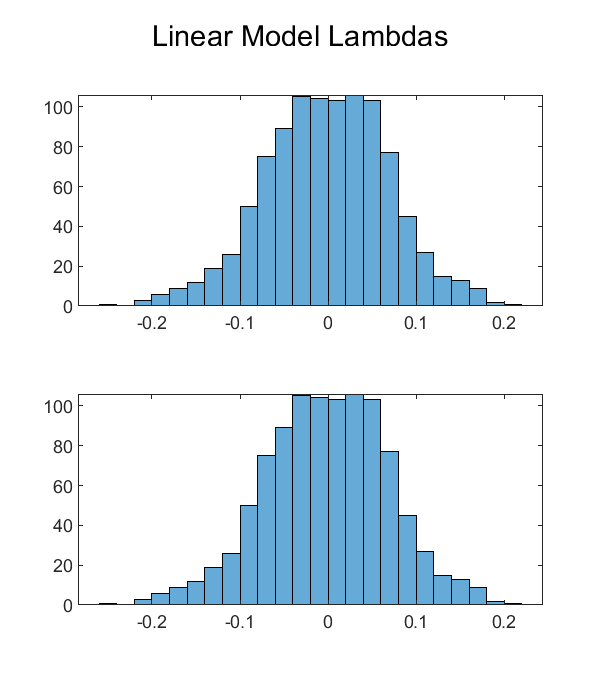
\includegraphics[scale=.3]{./tables/linear_lambdas_J1000_n200_kl1.png}

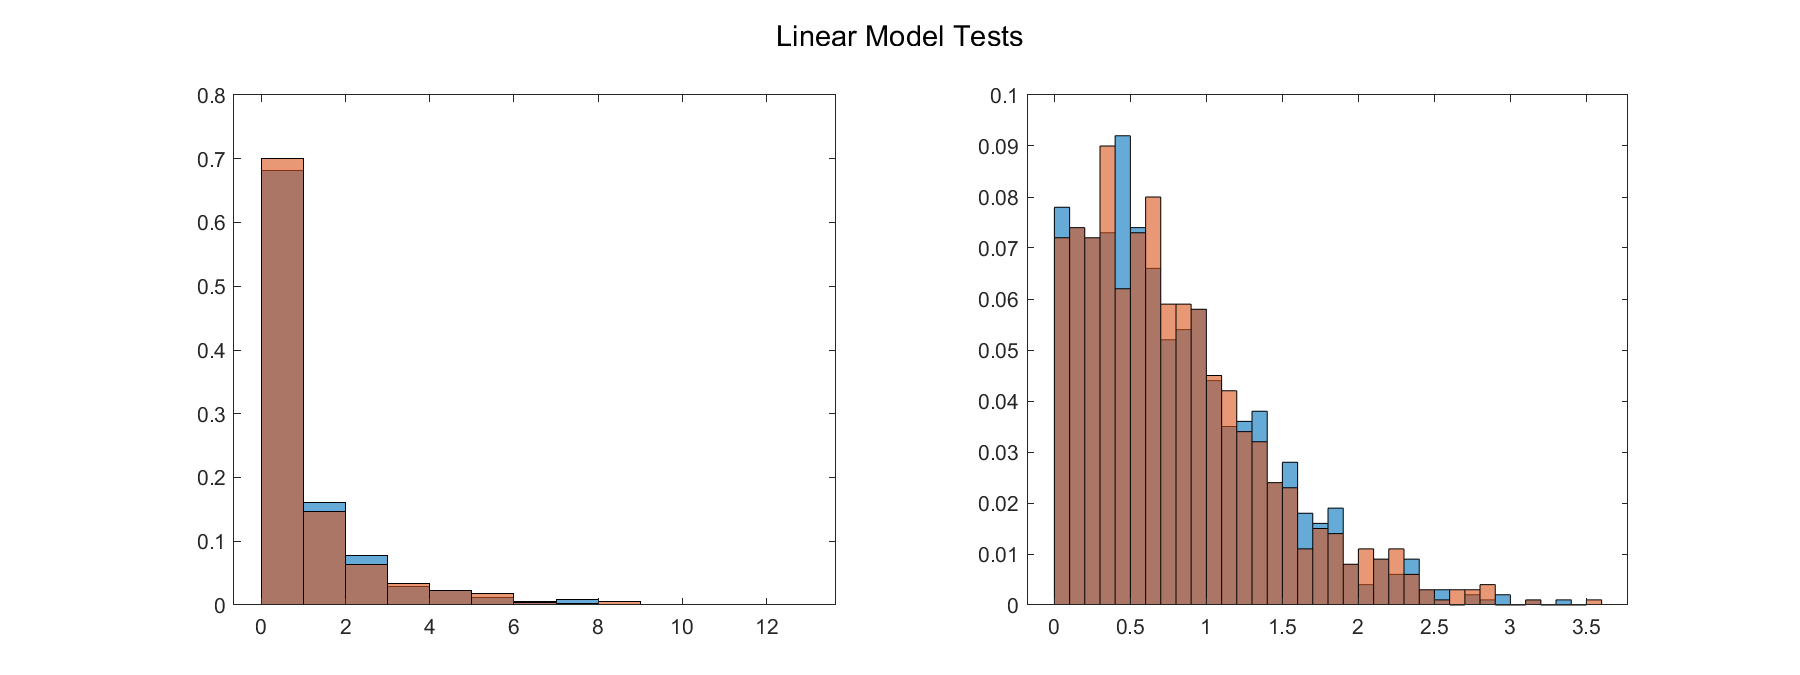
\includegraphics[scale=.3]{./tables/linear_tests_J1000_n200_kl1.png}
\end{center}

\vfill
\hfill 
\hyperlink{max_test_example_setup}{\beamergotobutton{Return to Example Setup}}
}

%

\frame{ 
\frametitle{}
\begin{center}
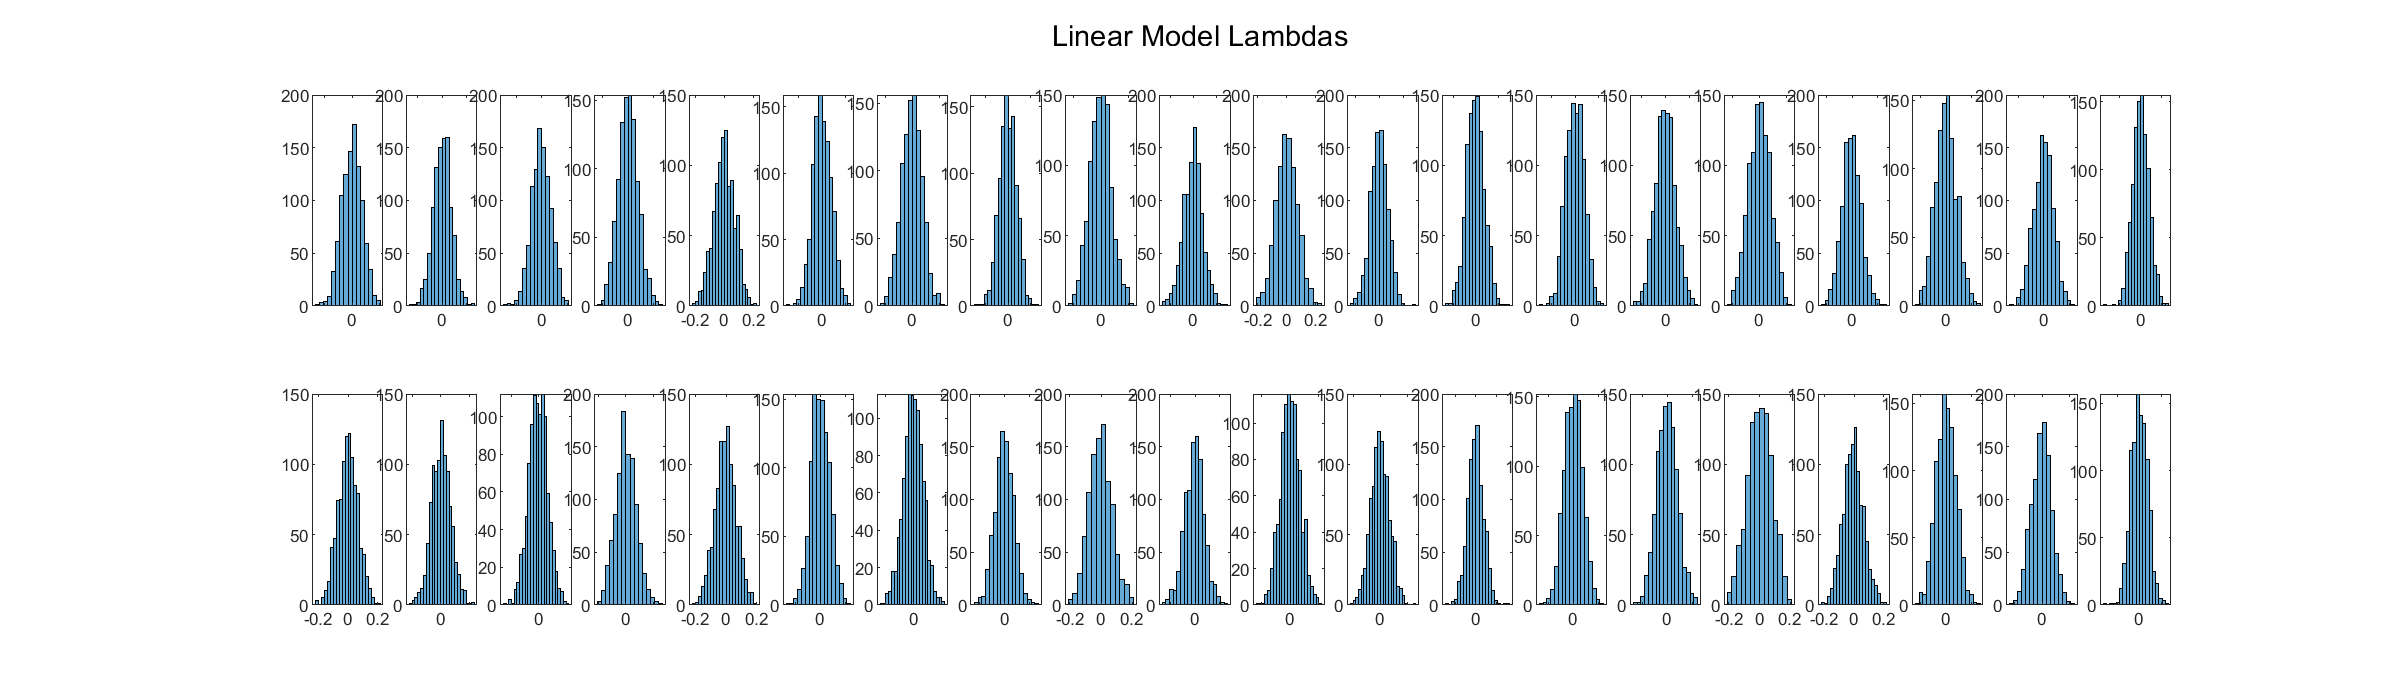
\includegraphics[scale=.3]{./tables/linear_lambdas_J1000_n200_kl20.png}

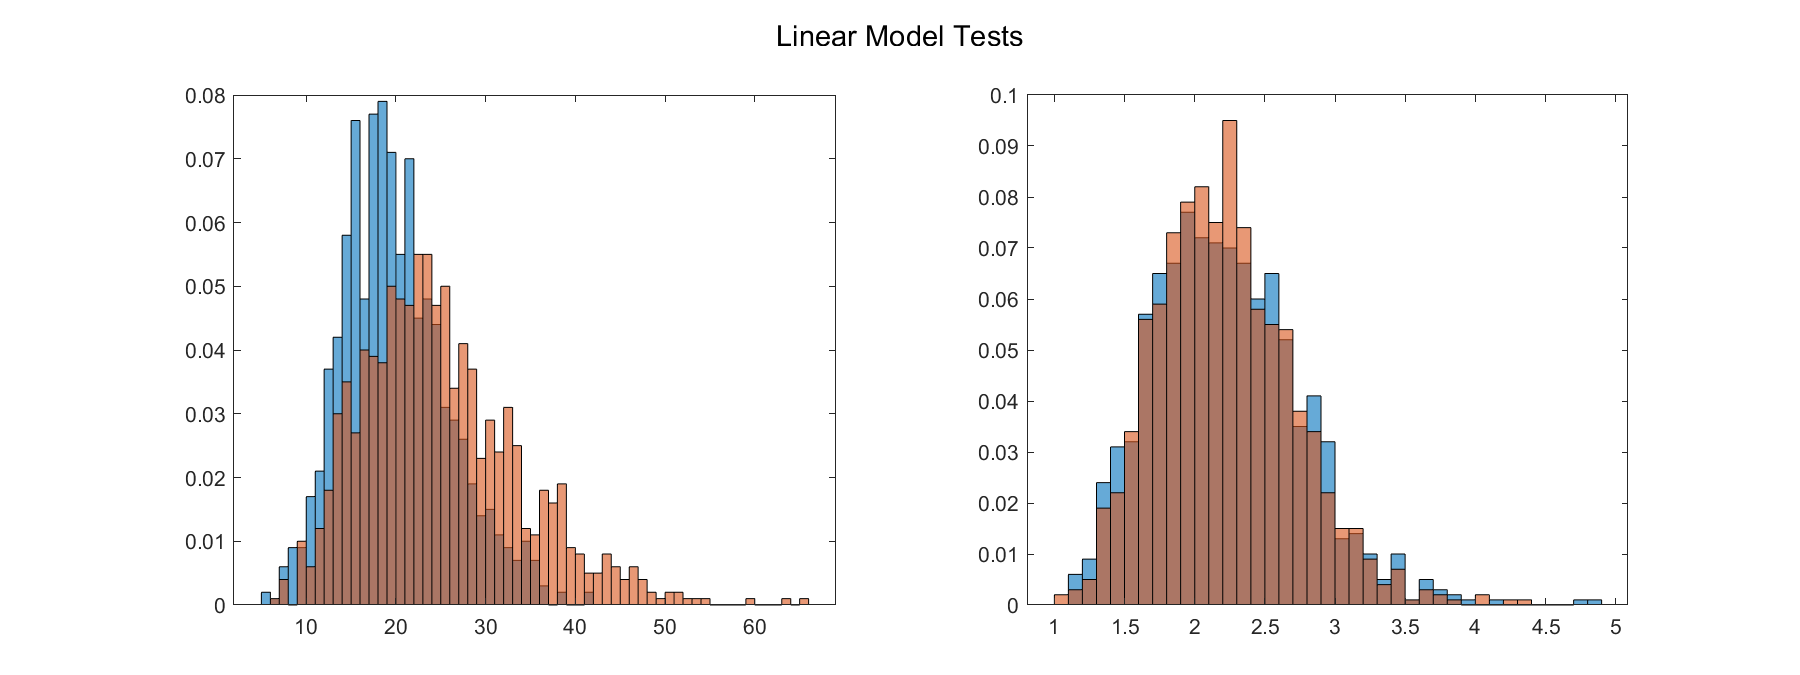
\includegraphics[scale=.3]{./tables/linear_tests_J1000_n200_kl20.png}
\end{center}

\vfill
\hfill 
\hyperlink{max_test_example_setup}{\beamergotobutton{Return to Example Setup}}
}

% 

\frame{ 
\frametitle{}
\begin{center}
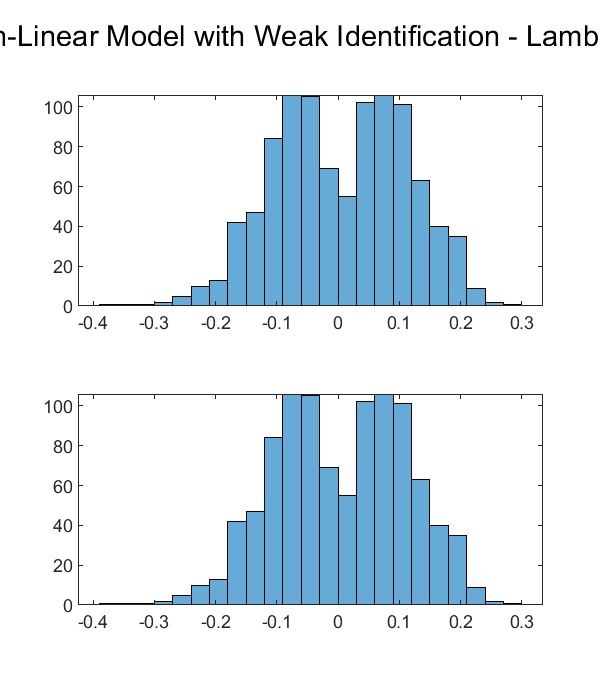
\includegraphics[scale=.3]{./tables/nonlinear_lambdas_J1000_n200_kl1.png}

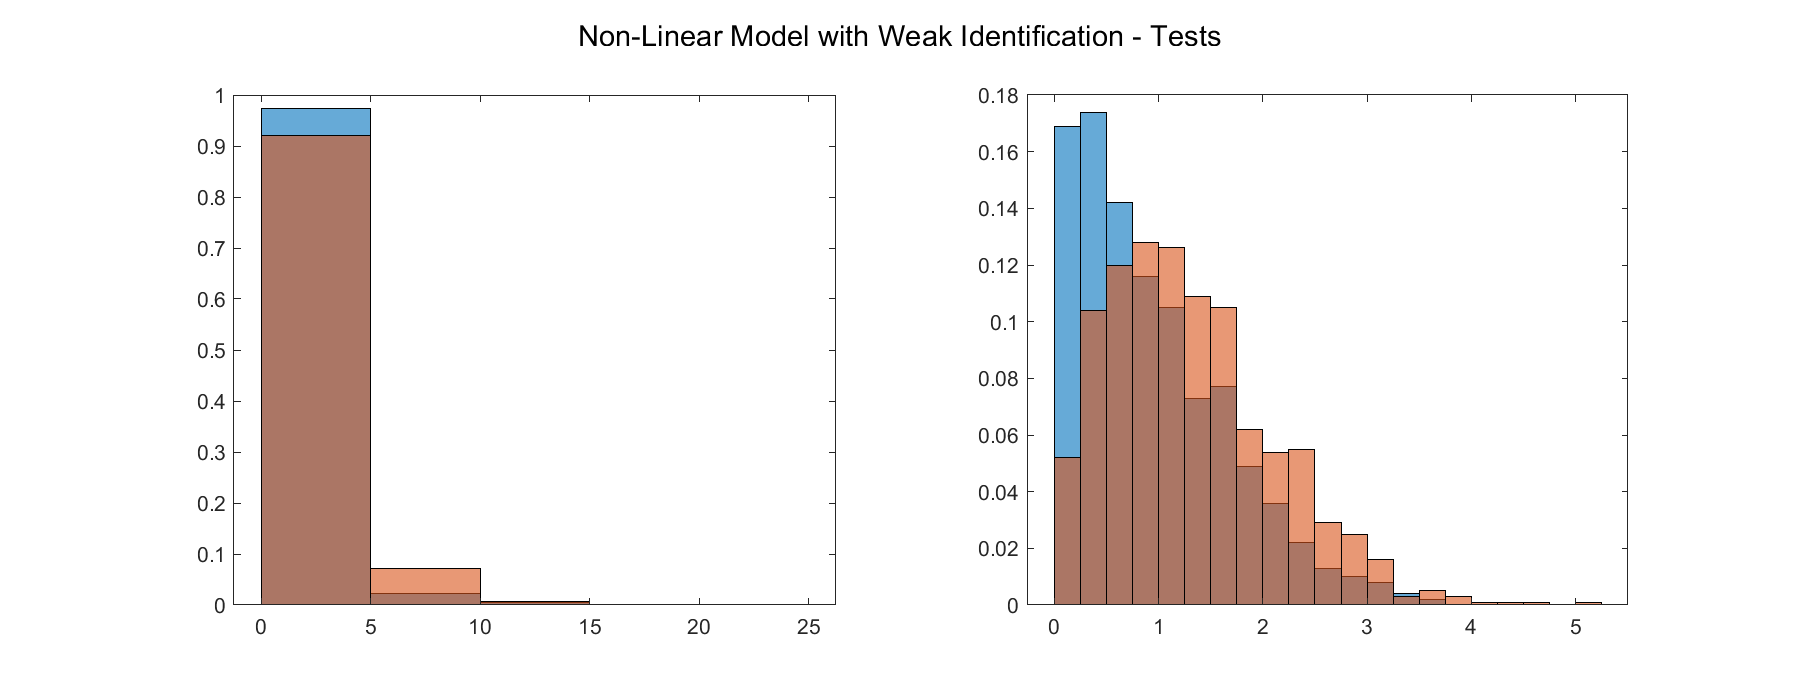
\includegraphics[scale=.3]{./tables/nonlinear_tests_J1000_n200_kl1.png}
\end{center}

\vfill
\hfill 
\hyperlink{max_test_example_setup}{\beamergotobutton{Return to Example Setup}}
}

%

\frame{ 
\frametitle{}
\begin{center}
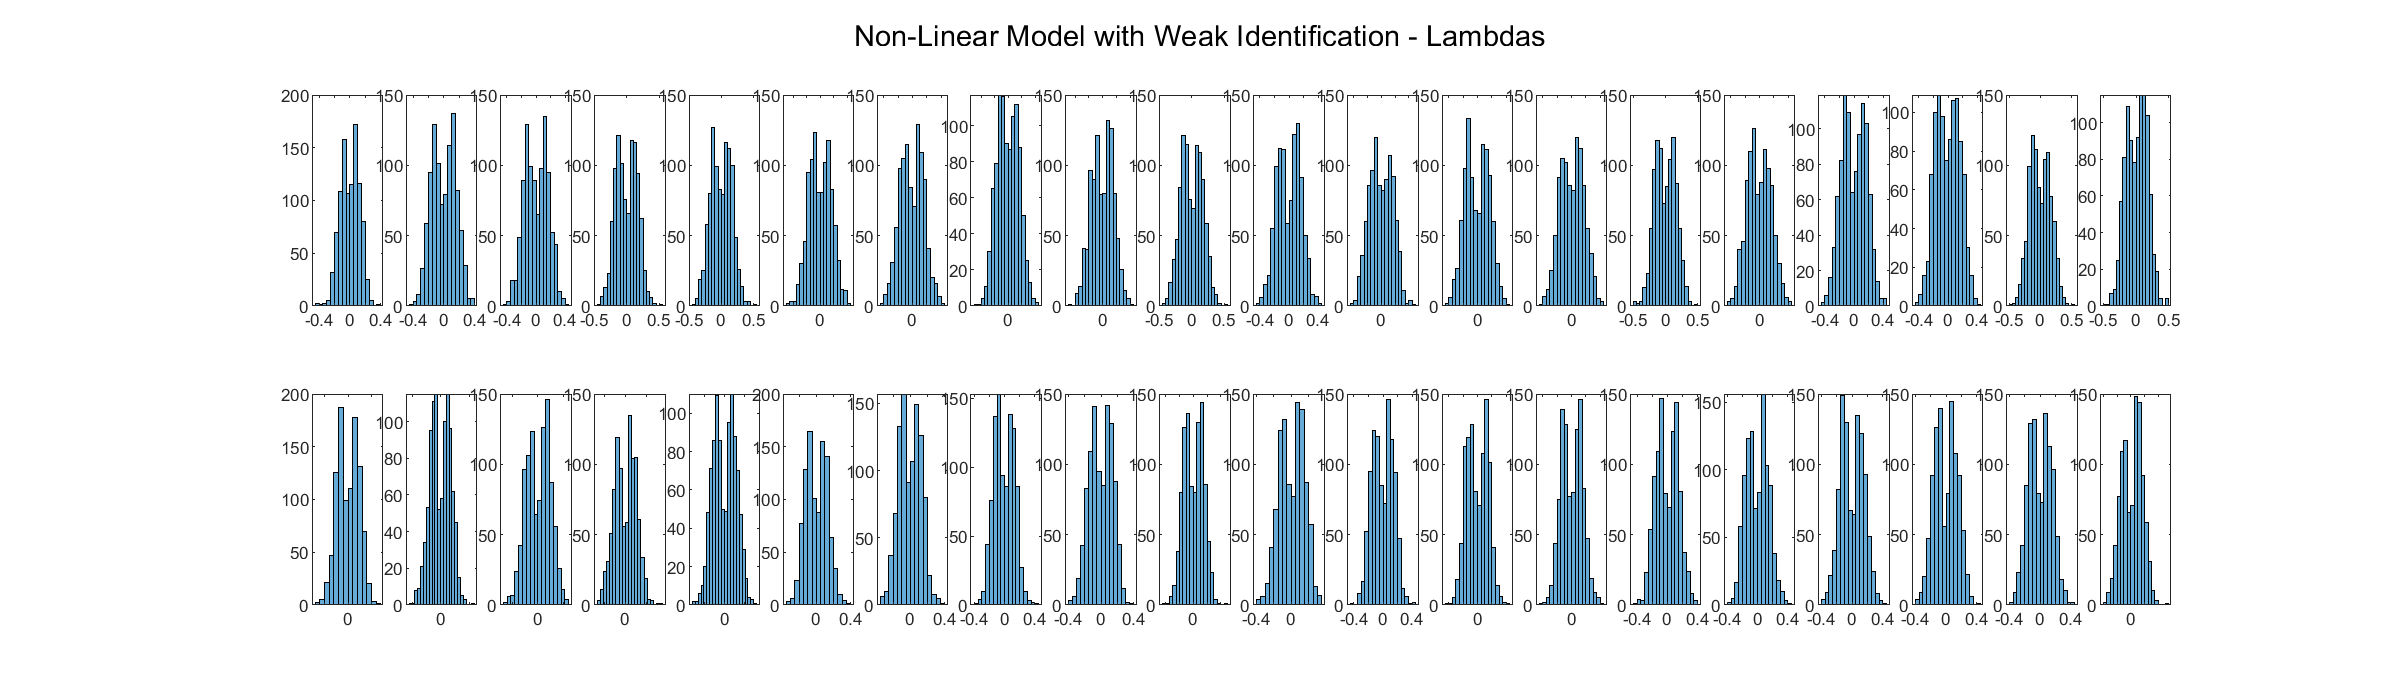
\includegraphics[scale=.3]{./tables/nonlinear_lambdas_J1000_n200_kl20.png}

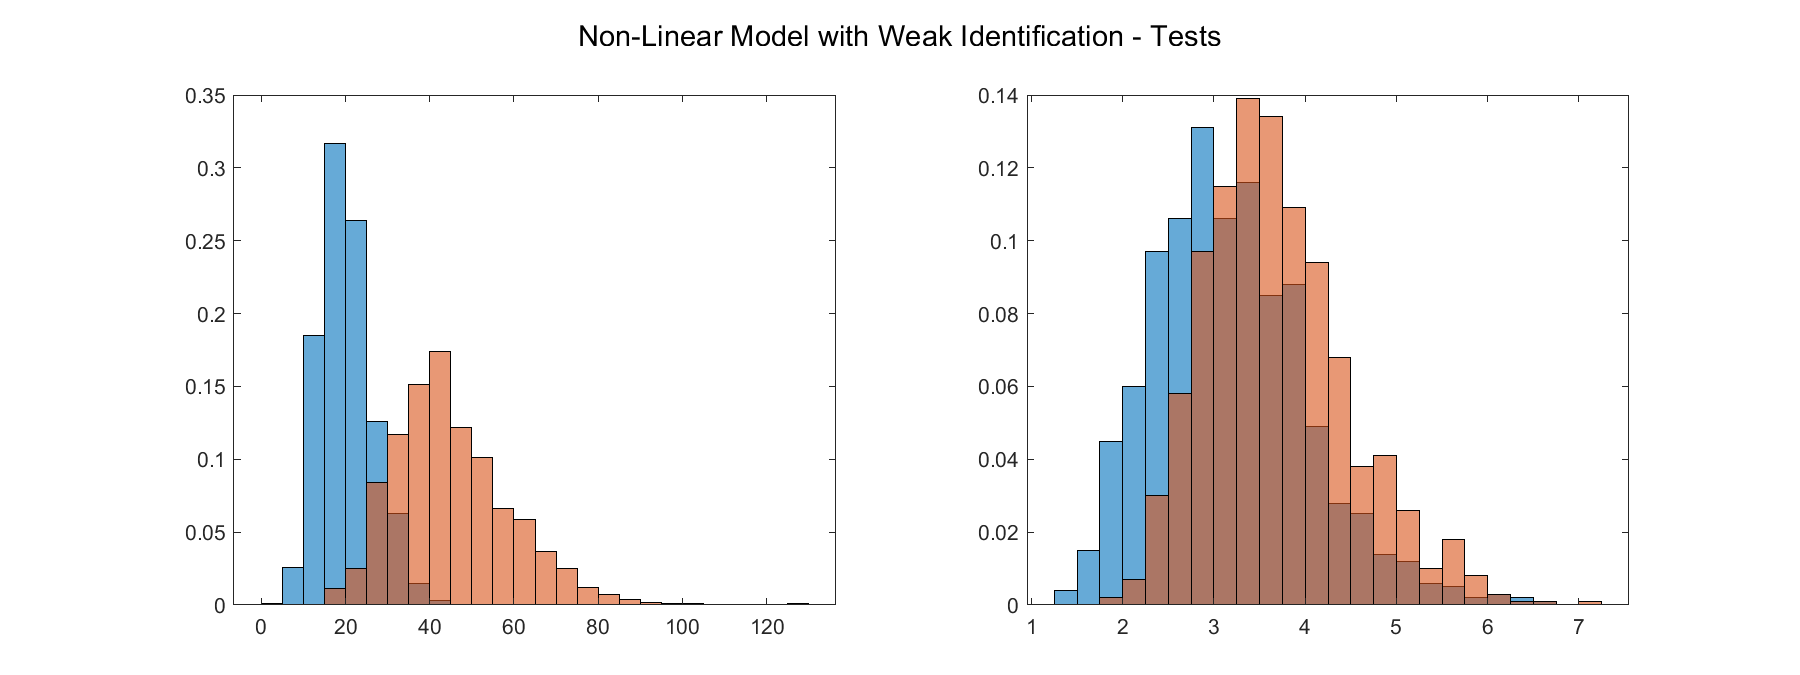
\includegraphics[scale=.3]{./tables/nonlinear_tests_J1000_n200_kl20.png}
\end{center}

\vfill
\hfill 
\hyperlink{max_test_example_setup}{\beamergotobutton{Return to Example Setup}}
}

% 

\frame[label = histogram_this_test]{ 
\frametitle{}
\begin{center}
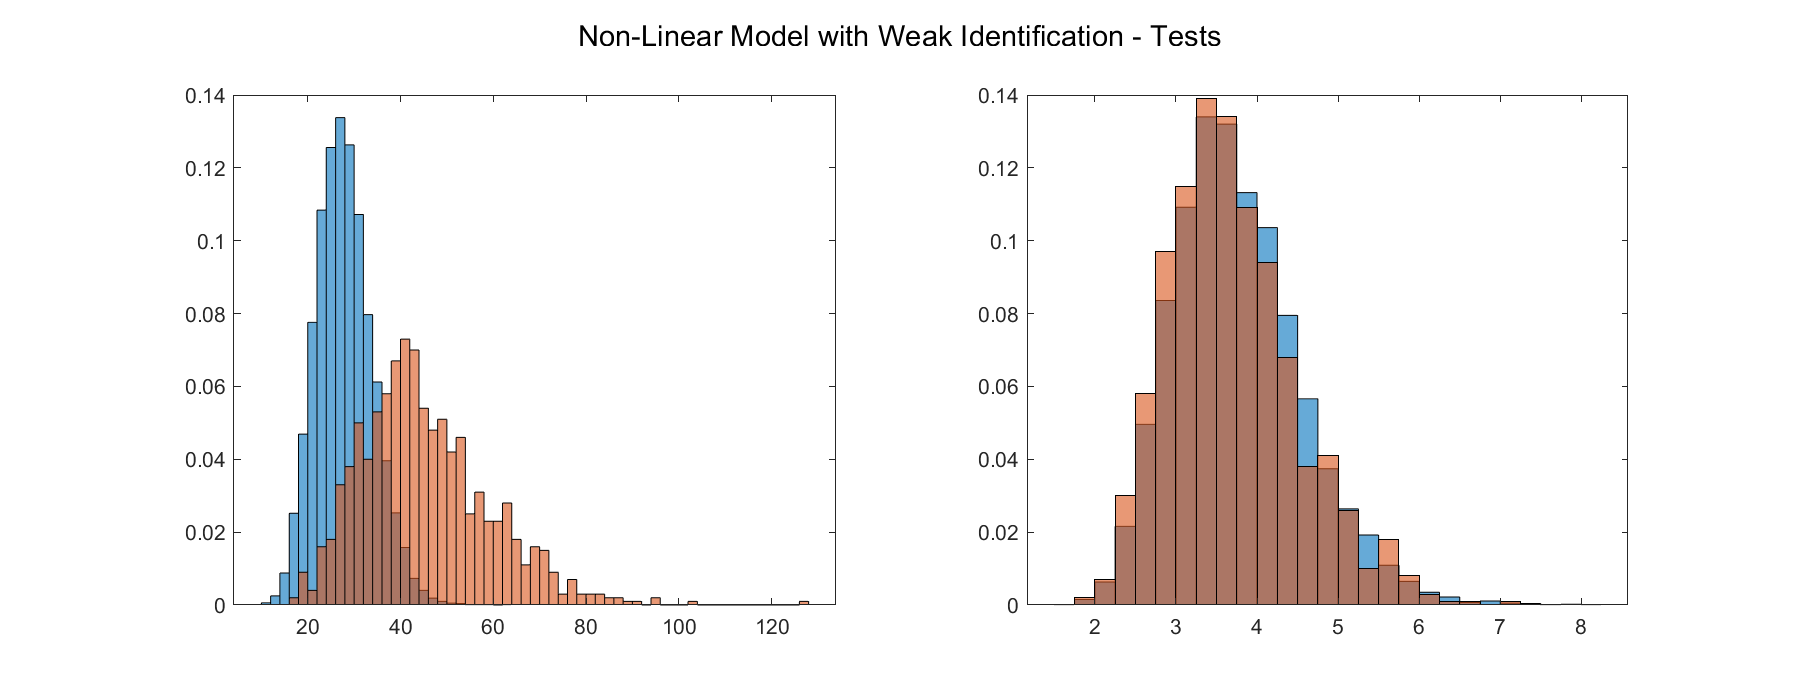
\includegraphics[scale=.3]{./tables/nonlinear_tests_this_paper_J1000_n200_kl20.png}
\end{center}

\vfill
\hfill 
\hyperlink{simulation_results}{\beamergotobutton{Return to Simulation Results}}
% \hyperlink{histogram_this_test}{\beamergotobutton{Histograms}}
}

%





\subsection*{Other Empirical Examples}


\frame[label = exchange_rate_pars_models_2]{
\frametitle{Empirical Example - Exchange Rate Modeling}
\begin{itemize}
\item Parsimonious model when $\lambda$ is a sub-vector of $\gamma$:
\begin{align*}
\Delta q_{t} = &
\Big[\delta_{\tilde{d},0} + \sum_{j=1}^{p} \delta_{\tilde{d},j} \Delta q_{t-j} \Big] h(\gamma_{\tilde{d}}, \Delta q_{t-\tilde{d}}) 
\\
& + \Big[\delta_{\highlight{d},0} + \sum_{j=1}^{p} \delta_{\highlight{d},j} \Delta q_{t-j} \Big] h(\lambda_{\highlight{d}}, \Delta q_{t-\highlight{d}}) 
+ u_{\highlight{d}, t}
\end{align*}
% \begin{align*}
% \Delta q_{t} = \sum_{i=0}^{p} \beta_{(d),i}^{*} g_{i}(\gamma_{d}, \Delta q_{t-d}) + u_{d,t}
% \end{align*}
\begin{itemize}
\item for each $d = 1, \dots, k$
% \item where $g_{i}(\gamma_{d}, \Delta q_{t-d}) = \Delta q_{t-i} h(\gamma_{d}, \Delta q_{t-d})$ for $i = 1, \dots, p$ 
% \item and $g_{0}(\gamma_{d}, \Delta q_{t-d}) = h(\gamma_{d}, \Delta q_{t-d})$.
\end{itemize}
\item Observe that $H_{0}$ $\Rightarrow$ $u_{d,t} = \e_{t}$ for every $d$
\end{itemize}
\vfill
\hfill 
\hyperlink{exchange_rate_pars_models_1}{\beamergotobutton{Return}}
}




%




\frame[label = example_linear_IV_LIML]{
\frametitle{Other Empirical Examples - LIML Linear IV}
\begin{itemize}
\item 
Linear IV with many instruments typically estimated with LASSO \citep{Belloni_Chernozhukov_Hansen_2010}

\item 
\cite{LeebPotscher2008,Potscher2009,Belloni_etal_2016} note that this can be problematic with many weak instruments


\item
Some new inference procedures address this.  For example, \cite{Belloni_Chernozhukov_Hansen_2014,BelloniChernozhukovHansen2014} perform a follow-up study regarding the effect of legalized abortion on crime


\item They alter \cite{DonohueLevitt2001} to include 284 variables with only 600 observations and illustrate `LASSO-double-selection'

\begin{itemize}
\item i) results based on a small set of intuitively selected controls differ from results obtained through formal variable selection
\item ii) accounting for nonlinear trends in the data affects the results
\end{itemize}

\item We can use the Max Test to examine if the `intuitively selected' or `added fidelity' controls are relevant.
\end{itemize}
}




\frame{
\frametitle{Other Empirical Examples - LIML Linear IV}

\begin{itemize}
\item Linear IV estimated by LIML fits into the weak identification framework
\citep{AndrewsCheng2012,AndrewsCheng2012_Supplemental}.  

\item We extend this to allow many covariates and instruments and mixed identification strength.

\vspace*{1cm}
\item
Related to LIML Linear IV weak instruments literature \citep{BoundJaegerBaker1996,AndrewsMoreiraStock2006,ChaoSwanson2007} etc...

\item
and the many weak instruments literature \cite{AndrewsStock2007} etc...

\item
and Post Selection Inference \citep{Belloni_Chernozhukov_Hansen_2014,BelloniChernozhukovHansen2014,Belloni_etal_2016}
\end{itemize}
}



\frame{
\frametitle{Other Empirical Examples - LIML Linear IV}
Consider the structural model
\begin{align*}
y_{t} = x_{1,t} \pi_{1} &+ x_{2,t} \pi_{2} + Z_{t}' \omega + u_{t}^{*}, \\
x_{1,t} = Z_{1,t}' \beta_{1} + v_{t}, 
&\qquad
x_{2,t} = Z_{2,t}' \beta_{2} + \eta_{t}.
\end{align*}

\vspace*{1cm}
The reduced form equations are
\begin{align*}
y_{t} &= Z_{1,t}' (\beta_{1} \pi_{1} + \omega_{1}) + Z_{2,t}' (\beta_{2} \pi_{2} + \omega_{2}) + u_{t}, \\
x_{1,t} &= Z_{1,t}' \beta_{1} + v_{t}, 
\quad
x_{2,t} = Z_{2,t}' \beta_{2} + \eta_{t}
\end{align*}
\begin{itemize}
\item 
where $u_{t} = v_{t}^{*} \pi_{1} + \eta_{t}^{*} \pi_{2} + u_{t}^{*}$, 

\item
and we assume $(u_{t}, v_{t}, \eta_{t}) \sim N(0, \Sigma)$.
\end{itemize}
}





\frame{
\frametitle{Other Empirical Examples - LIML Linear IV}
\begin{itemize}
\item We can use the Max Test to examine if the `intuitively selected' or `added fidelity' controls are relevant.

\item e.g. $H_{0}: (\beta_{2}, \omega_{2}) = 0_{k}$ for large $k$

\item The Parsimonious models are the reduced form equations
\begin{align*}
y_{t} &= Z_{1,t}' (\beta_{1} \pi_{1} + \omega_{1}) + Z_{2,\highlight{i},t} (\beta_{2,\highlight{i}} \pi_{2}) + \tilde{u}_{(i),t}, 
\\
x_{1,t} &= Z_{1,t}' \beta_{1} + v_{t} \\
x_{2,t} &= Z_{2,\highlight{i},t} \beta_{2,\highlight{i}} + \tilde{\eta}_{(i),t}
\end{align*}
and
\begin{align*}
y_{t} &= Z_{1,t}' (\beta_{1} \pi_{1} + \omega_{1}) + Z_{2,\highlight{i},t} \omega_{2,\highlight{i}} + \tilde{w}_{(i),t}, 
\\
x_{1,t} &= Z_{1,t}' \beta_{1} + v_{t}
\end{align*}
\end{itemize}
}


\frame{
\frametitle{Other Empirical Examples - LIML Linear IV}
\begin{itemize}
\item let $\lambda = \beta_{2}$, and consider $H_{0}: \lambda = 0$:
\end{itemize}
\vspace*{1cm}
\highlight{REWRITE THIS}
\begin{equation*}
\left.\begin{aligned}
y_{t} &= Z_{1,t}' \beta_{1} \pi_{1} + Z_{2,\highlight{1},t} \lambda_{\highlight{1}} \pi_{2} + u_{t} \\
x_{1,t} &= Z_{1,t}' \beta_{1} + v_{t} \\
x_{2,t} &= Z_{2,\highlight{1},t} \lambda_{\highlight{1}} + \tilde{\eta}_{1,t}
 \\
 & \hspace*{1cm} \vdots \\
y_{t} &= Z_{1,t}' \beta_{1} \pi_{1} + Z_{2,\highlight{k},t} \lambda_{\highlight{k}} \pi_{2} + u_{t} \\
x_{1,t} &= Z_{1,t}' \beta_{1} + v_{t} \\
x_{2,t} &= Z_{2,\highlight{k},t} \lambda_{\highlight{k}} + \tilde{\eta}_{k,t}
\end{aligned}\right\}
\hspace*{.3cm}
\Rightarrow
\hspace*{.3cm}
\left.\begin{aligned}
\hat{\lambda}_{1} \\ \vdots \\ \hat{\lambda}_{k}
\end{aligned}\right\}
\hspace*{.3cm}
\Rightarrow
\hspace*{.3cm}
\hat{\Tc} = \max_{1\le i \le k} |\Ns_{i} \hat{\lambda}_{i}|
\end{equation*}
\vfill 
\hfill 
\hyperlink{examples_other}{\beamergotobutton{Back to Empirical Examples}}
}



















\subsection*{Limiting Distribution}

\frame{
\frametitle{Appendix - Grouping Notation}
\begin{itemize}
\item Parameters are grouped based on identification strength.
\item Weakly identified parameters are placed in group $l_{K}$
\end{itemize}
}



\frame[allowframebreaks]{
\frametitle{Appendix - Limiting Distribution}

let $\G_{(i)}(\pi_{(i), l_{K}}; \gamma_{0})$ be a zero mean Gaussian process with covariance kernel $\Omega_{(i)}(\pi_{(i), l_{K}}, \tilde{\pi}_{(i), l_{K}}; \gamma_{0})$, and define the processes
\begin{align}
\tau_{(i)}(\pi_{(i), l_{K}}; \gamma_{0}) 
&= \Big[ H_{(i), K}(\pi_{(i), l_{K}}; \gamma_{0}) \Big]^{-1} \Big( \K_{(i), K}(\pi_{(i), l_{K}}; \gamma_0) b_{(i), l_{K}} + \G_{(i)}(\pi_{(i), l_{K}}; \gamma_{0}) \Big) \label{E:Definition of Tau} \\
\chi_{(i)}(\pi_{(i), l_{K}}; \gamma_{0}) 
&= -\frac{1}{2} \tau_{(i)}(\pi_{(i), l_{K}}; \gamma_{0})'
 \Big[ H_{(i), K}(\pi_{(i), l_{K}}; \gamma_{0}) \Big]
 \tau_{(i)}(\pi_{(i), l_{K}}; \gamma_{0}). \label{E:Definition of Chi} 
\end{align}


\begin{theorem}[5.4] \label{T:Pointwise Asymptotic Distribution of the Parsimonious Estimators}
Let Assumptions 1-8 hold.
Under $\gamma_n \to \gamma_0$, 
\begin{enumerate}[a)]
\item If $l_{K} \ne \emptyset$, where $l_{K}$ indexes the weakly identified subvector of $\pi_{(i)}$, then
\begin{align} \label{E: Asymptotic Distribution of Parsimonious Estimators a.i}
n \big( Q_{(i), n}^{c}(\pi_{(i), l_{k}}) - Q_{(i), n}(\psi_{(i), K,n}^{0}, \pi_{(i), l_{k}}) \big) 
& \Rightarrow \chi_{(i)}(\pi_{(i), l_{K}}; \gamma_{0}) \\
%
\pmat{n^{1/2} B(\beta_{(i), K^{-},n}) \big( \hat{\psi}_{(i), K^{-}} - \psi_{(i), K^{-},n} \big) \\ \hat{\pi}_{(i), l_{K}}} 
& \tod
\pmat{\tau_{(i)}(\pi_{(i), l_{K}}^{*}) - S_{l_{K}} b_{(i), l_{K}} \\ \pi_{(i), l_{K}}^{*}}
\label{E: Asymptotic Distribution of Parsimonious Estimators a.ii}
\end{align}
where $S_{l_{K}}$ is the selection matrix that selects the columns corresponding to $\beta_{(i), l_{k}}$.

\item if $l_{k} = \emptyset$, then no parameters are weakly identified, so $\beta_{(i), K^{-},n} = \beta_{(i), n}$ and
\begin{align}
n \big( Q_{(i), n}(\hat{\theta}_{(i)}) - Q_{(i), n}(\theta_{(i), n}) \big) 
& \tod \chi_{(i), \theta}(\gamma_{0}) \\
%
n^{1/2} B(\beta_{(i), n}) (\hat{\theta}_{(i)} - \theta_{(i), n}) 
& \tod 
H_{(i), K-1}(\gamma_{0})^{-1} \G_{(i), \theta}(\gamma_{0})
\end{align}
where $\G_{(i), \theta}(\gamma_{0}) \sim N(0, \Omega_{(i), \theta}(\gamma_{0}))$, and $\chi_{(i), \theta}(\gamma_{0}) = -\frac{1}{2} \G_{(i), \theta}(\gamma_{0})' H_{(i), K-1}(\gamma_{0})^{-1} \G_{(i), \theta}(\gamma_{0})$.
% where $G_{(i), \theta}(\gamma_{0}) \sim N(0, \Sigma_{(i)}(\gamma_{0}))$ and $\Sigma_{(i)}(\pi_{0}, \omega_{0}) = H_{(i), K-1}(\gamma_{0})^{-1} \Omega_{(i), \theta}(\gamma_{0}) H_{(i), K-1}(\gamma_{0})^{-1}$.
\end{enumerate}
\end{theorem}


\begin{theorem}[5.5]\label{T:Joint Asymptotic Distribution of the Parsimonious Estimators}
Let $\gamma_{n} \to \gamma_{0}$ and suppose Assumptions 1-7 and 9 hold.  Then
\begin{equation*}
\Bigg\{ 
n^{1/2} B_{(i)}(\beta_{(i), n}) \pmat{ ( \hat{\psi}_{(i), K^{-}} - \psi_{(i), K^{-},n} ) \\ \hat{\pi}_{(i), l_{K}} - \pi_{(i), l_{K}, 0} }
 : \ 1\le i \le \mathring{k} \Bigg\}
\tod
\Bigg\{ 
\mathfrak{Z}_{(i)} : \ 1\le i \le \mathring{k} \Bigg\},
\end{equation*}
where $\mathfrak{Z}_{(i)}$ are defined point-wise as in Theorem \ref{T:Pointwise Asymptotic Distribution with normalization for consistency} for each $i$.
%, and covariance given by $E_{\gamma_{0}}[\mathfrak{Z}_{(i)} \mathfrak{Z}_{(j)}']$
\end{theorem}


\begin{theorem}\label{T:Test stat limiting distribution}
Let Assumptions 1-7, 9, and 10 hold, and let $\mathfrak{Z}_{(i)}$ be as in Theorem \ref{T:Joint Asymptotic Distribution of the Parsimonious Estimators}.  Then under $H_{0}$,
\begin{equation*}
\Big| \hat{\Ts}_{n} - \max_{1\le i \le \mathring{k}_{n}} |S_{(i), \lambda}' W_{(i)} \mathfrak{Z}_{(i)}| \Big| \toP 0
\end{equation*}
for some non-unique $\mathring{k}_{n} = o(n)$.
\end{theorem}

}







\subsection*{Max Tests}

\frame[label = max_tests_explanation_slide]{
\frametitle{Max Tests}
\begin{align*}
\hat{\mathcal{T}}_{n} = \max_{1 \le i \le k_{n}} | \sqrt{n} \hat{\lambda}_{i,n}|
\end{align*}
\begin{itemize}
\setlength\itemsep{.25cm}
\item do not require inversion of a large covariance matrix
\item Utilize the most informative of a sequence of estimators
%\begin{itemize}
%\item avoids issue of washing out the influence of a single non-zero estimate
%\end{itemize}
\item trade-off: ignore information from everything that is not the maximum
\citep{Hansen2005_JBES}
\hfill 
\hyperlink{correlation_examples}{\beamergotobutton{Example}}
\hyperlink{correlation_examples_combo}{\beamergotobutton{Example 2}}
\end{itemize}

\vfill
\hfill 
\hyperlink{Initial_simulation_evidence}{\beamergotobutton{Return to Intro}}
\hyperlink{what_we_can_and_cant_test}{\beamergotobutton{Return to Caveats}}
}




\frame[label = correlation_examples]{
\frametitle{Max Tests - Correlation Examples}
%\begin{center}
\hspace*{-1.25cm}
\includegraphics[scale=.35]{./fig/rho_example_J100.png}
%\end{center}

\hfill 
\hyperlink{correlation_examples_combo}{\beamergotobutton{Combining Correlations}}
\hyperlink{max_tests_explanation_slide}{\beamergotobutton{Go back}}
}


\frame[label = correlation_examples_combo]{
\frametitle{Max Tests - Max Correlation Examples}
%\begin{center}
\hspace*{-1.25cm}
\includegraphics[scale=.35]{./fig/combinations_rho_example_J100.png}
%\end{center}

$H_0: \rho_n = 0 \quad \forall n$ 
\hfill
\hyperlink{max_tests_explanation_slide}{\beamergotobutton{Go back}}
}





\subsection{Test Statistic}

\frame[label = Test_stat_theorem]{
\frametitle{Appendix - Test Statistic}
\begin{itemize}
\item Take away: Distributions are different $\Rightarrow$ possibility of distorted inference when ignoring possibility of identification failure
\begin{itemize}
\item Under Strong Id, the limit is standard
\item Under Weak Id, $\hat{\pi}_n$ is not consistent, and the limiting distribution is complicated!
\end{itemize}
\item We will bootstrap these distributions...
\hfill 
\hyperlink{bootstrapping_the_max_test_is_new}{\beamergotobutton{Bootstapping a Max Statistic?}}
\end{itemize}

\vfill \hfill \hyperlink{critical_values_short_slide}{\beamergotobutton{Return to CV slide}}
}





\subsection*{Bootstrap}

\frame[label = Inference_sim_step_2b]{
\frametitle{Appendix - Inference Procedure Step 2b}
\begin{enumerate}
\item 
The bootstrapped quantities with weakly identified parameters:
\begin{align*}
\hat{\G}_{(i)}^{bs}(\pi_{(i), l_{K}}) 
= \frac{1}{\sqrt{n}} \sum_{t=1}^{n} z_{t} \Big\{ m_{(i),t}(\hat{\psi}_{(i), K^{-},n}^{0}(\pi_{(i), l_{K}}), \pi_{(i), l_{K}}) - \frac{1}{n} \sum_{t=1}^{n} m_{(i),t}(\hat{\psi}_{(i), K^{-},n}^{0}(\pi_{(i), l_{K}}), \pi_{(i), l_{K}}) \Big\}.
\end{align*}
Use this to form the quantities
\begin{align*}
\hat{\tau}_{(i)}^{bs}(\pi_{(i), l_{K}}; \gamma_0, b) 
&= \Big[ \hat{H}_{(i), K}(\pi_{(i), l_{K}}) \Big]^{-1} \Big( \hat{\K}_{(i), K}(\pi_{(i), l_{K}}; \gamma_0) b_{(i), l_{K}} + \hat{\G}_{(i)}^{bs}(\pi_{(i), l_{K}}) \Big) \\
\hat{\chi}_{(i)}^{bs}(\pi_{(i), l_{K}}; \gamma_0, b) 
&= -\frac{1}{2} \hat{\tau}_{(i)}^{bs}(\pi_{(i), l_{K}}; \gamma_0, b)'
 \Big[ \hat{H}_{(i), K}(\pi_{(i), l_{K}}) \Big]
 \hat{\tau}_{(i)}^{bs}(\pi_{(i), l_{K}}; \gamma_0, b) 
\end{align*}
Next, compute 
\begin{align*}
\pi_{(i), l_{K}}^{*, bs}(\gamma_0, b) = \argmin_{\pi_{(i), l_{K}} \in \Pi_{(i), l_{K}}} \hat{\chi}_{(i)}^{bs}(\pi_{(i), l_{K}}; \gamma_0, b).
\end{align*}
\end{enumerate}
\hfill \hyperlink{Inference_Procedure_sim}{\beamergotobutton{ Inference Procedure}}
}




\frame[label = bootstrap_summary_weak_id]{
\frametitle{Appendix - Bootstrap Overview}
\textbf{Weak Identification:}
\begin{enumerate}
\item Simulate a random draw, $\pi^*_{(bs)}(b, \pi_0)$, from the distribution $\pi^*(b, \pi_0)$ using the $z_t$
\item Use $\pi^*_{(bs)}(b, \pi_0)$ to construct the components of our test statistic under weak identification, which are functions of $\pi$.  
\item Use the draws $z_t$ to construct the wild bootstrap version of the test statistic.  
\item deal with nuisance parameters $b$ and $\pi_0$
\end{enumerate}
\hfill \hyperlink{bootstrap_algorithm_weak_id}{\beamergotobutton{Go to the Bootstrap Algorithm for Weak Id}}

\textbf{Strong Identification:}
\begin{enumerate}
\item Construct the components of our test statistic using $\hat{\theta}_n$.  
\item Use the draws $z_t$ to construct the wild bootstrap version of the test statistic.  
\end{enumerate}
\hfill \hyperlink{bootstrap_algorithm_strong_id}{\beamergotobutton{Go to the Bootstrap Algorithm for Strong Id}}
}


\subsubsection{Critical Value Computation}

\frame[label = cv_computation_summary]{
\frametitle{Appendix - Critical Value Computation Overview}
\begin{enumerate}
\item Repeat the above procedures $M$ times for each identification category.
\item Order the resulting test statistics within each category.
\item $\alpha$-level critical values are the statistics in $[(1-\alpha)\cdot M]$th ordered positions
\item The critical value under weak identification depends on nuisance parameters.  Sup over these nuisance parameters.
\end{enumerate}
\hfill 
\hyperlink{cv_computation}{\beamergotobutton{Go To Critical Value Computation Algorithm}}

\vfill \hfill \hyperlink{critical_values_short_slide}{\beamergotobutton{Return to CV slide}}
}



\subsection{Robust Critical Values}


\frame[label = robust_cvs]{
\frametitle{Appendix - Putting the Critical Values Together}
Robust Critical Values:
\begin{itemize}
\item Least Favorable (LF)
\begin{itemize}
\item always take the larger of the critical values
\item $c_{1-\alpha}^{(LF)} = \max\{ c_{1-\alpha}^{(w)}, c_{1-\alpha}^{(s)} \}$
\end{itemize}

\vspace*{.5cm}
\item Identification-Category Selection (ICS) 
\begin{itemize}
\item data driven pre-test for the id category
\item Step 1: Use data to determine if $b = \lim_{n} \sqrt{n} \beta_n$ is finite
\item Step 2:
\begin{itemize}
\item if we believe $b$ is finite, use $LF$ cv
\item otherwise, use (semi-) Strong identification cv
\end{itemize}
\hfill 
\hyperlink{ICS_cv_details}{\beamergotobutton{Go To ICS Details}}
\end{itemize}
\end{itemize}

\vspace{1cm}
Decision Rule: Reject the null hypothesis when $\hat{T}_n > c_{1-\alpha}^{(\cdot)}$.

\vfill \hfill \hyperlink{critical_values_short_slide}{\beamergotobutton{Return to Inference}}
}




\frame[label = ICS_cv_details]{
\frametitle{ICS Critical Values}
The statistic used for category selection is 
\begin{equation*}
\A_n = (n \hat{\beta}_n' \hat{\Sigma}_{\beta \beta, n}^{-1} \hat{\beta}_n / d_{\beta})^{1/2}
\end{equation*}
where $\hat{\Sigma}_{\beta \beta, n}$ is the upper left $d_{\beta} \times d_{\beta}$ block of $\hat{\Sigma}_{n} = \hat{J}_n^{-1} \hat{V}_n \hat{J}_n^{-1}$, the estimator of the strong identification covariance matrix $\Sigma(\gamma_0) = J^{-1} V J^{-1}$.

Let $\{\kappa_n: \ n\ge 1\}$ be a sequence of constants s.t. 
\begin{equation*}
\kappa_n \to \infty \qquad \text{and} \qquad \kappa_n / n^{1/2} \to 0
\end{equation*}

The ICS critical value is $c_{1-\alpha}^{(ICS)} = \begin{cases}
c_{1-\alpha}^{(LF)} & \qquad \text{if} \ \A_n \le \kappa_n \\ 
c_{1-\alpha}^{(s)} & \qquad \text{if} \ \A_n > \kappa_n
\end{cases}$

\hfill 
\hyperlink{robust_cvs}{\beamergotobutton{Return to CV Overview}}
}





\subsection*{Simulations}

\frame[label = simulation_results_null_table_full]{
% \frametitle{Simulation Results}
 \begin{table}[H] 
 \singlespacing 
 \tiny 
 \centering 
\begin{tabular}{c|cccccc|cccccc} 
\multicolumn{13}{c}{ Rejection Frequencies, Experiment: 1, DGP: 2, Hyp: Null } \\ 
\multicolumn{13}{c}{ $n=200$, $J=10000$, $\alpha = 0.05$ } \\ 
 \multicolumn{1}{c}{} & \multicolumn{6}{c}{ $k_{\lambda,n}=1$ } & \multicolumn{6}{c}{ $k_{\lambda,n}=20$ } \\ 
 \hline 
 $b_{1}$ & $0$ & $1$ & $2$ & $5$ & $10$ & $14$ & $0$ & $1$ & $2$ & $5$ & $10$ & $14$   \\ 
 \hline 
 \hline 
 Wald Test Standard &  0.11 &  0.12 &  0.12 &  0.13 &  0.12 &  0.12 &  0.83 &  0.84 &  0.83 &  0.83 &  0.84 &  0.84 \\ 
 Max Test Standard &  0.10 &  0.10 &  0.10 &  0.10 &  0.10 &  0.10 &  0.12 &  0.11 &  0.11 &  0.11 &  0.11 &  0.11 \\ 
 Max t-Test Standard &  0.11 &  0.12 &  0.11 &  0.11 &  0.11 &  0.11 &  0.19 &  0.19 &  0.19 &  0.19 &  0.20 &  0.20 \\ 
 \hline 
 Wald Test BS1 &  0.06 &  0.06 &  0.06 &  0.06 &  0.06 &  0.06 &  0.68 &  0.68 &  0.67 &  0.68 &  0.69 &  0.69 \\ 
 Max Test BS1 &  0.04 &  0.04 &  0.04 &  0.04 &  0.04 &  0.04 &  0.03 &  0.03 &  0.03 &  0.03 &  0.03 &  0.03 \\ 
 Max t-Test BS1 &  0.06 &  0.06 &  0.06 &  0.06 &  0.06 &  0.06 &  0.13 &  0.12 &  0.13 &  0.13 &  0.13 &  0.13 \\ 
 \hline 
 Wald Test BS2 &  0.06 &  0.06 &  0.06 &  0.06 &  0.06 &  0.06 &  0.25 &  0.26 &  0.26 &  0.26 &  0.25 &  0.25 \\ 
 Max Test BS2 &  0.05 &  0.05 &  0.05 &  0.05 &  0.05 &  0.05 &  0.04 &  0.04 &  0.04 &  0.04 &  0.04 &  0.04 \\ 
 Max t-Test BS2 &  0.06 &  0.06 &  0.06 &  0.06 &  0.06 &  0.06 &  0.08 &  0.08 &  0.08 &  0.08 &  0.08 &  0.09 \\ 
 \hline 
 Wald Test Taylor &  0.09 &  0.09 &  0.09 &  0.09 &  0.09 &  0.09 &  0.52 &  0.52 &  0.52 &  0.52 &  0.52 &  0.52 \\ 
 Max Test Taylor &  0.60 &  0.60 &  0.60 &  0.60 &  0.60 &  0.60 &  0.99 &  0.99 &  0.99 &  0.99 &  0.99 &  0.99 \\ 
 Max t-Test Taylor &  0.09 &  0.09 &  0.09 &  0.09 &  0.09 &  0.09 &  0.16 &  0.16 &  0.16 &  0.16 &  0.16 &  0.16 \\ 
 \hline 
\end{tabular}
 \end{table}

\vfill 
\hfill
\hyperlink{simulation_results_null_table}{\beamergotobutton{Back to table}}
}

\frame{
\frametitle{Simulation Results}
 \begin{table}[H] 
 \singlespacing 
 \tiny 
 \centering 
\begin{tabular}{c|cccccc|cccccc} 
\multicolumn{13}{c}{ Rejection Frequencies, Experiment: 1, DGP: 2, Hyp: Local Alternative } \\ 
\multicolumn{13}{c}{ $n=200$, $J=10000$, $\alpha = 0.05$ } \\ 
  \multicolumn{1}{c}{} & \multicolumn{6}{c}{ $k_{\lambda,n}=1$ } & \multicolumn{6}{c}{ $k_{\lambda,n}=20$ } \\ 
 \hline 
 $b_{1}$ & $0$ & $1$ & $2$ & $5$ & $10$ & $14$ & $0$ & $1$ & $2$ & $5$ & $10$ & $14$   \\ 
 \hline 
 \hline 
 Wald Test Standard &  0.21 &  0.22 &  0.20 &  0.22 &  0.21 &  0.21 &  0.91 &  0.91 &  0.90 &  0.91 &  0.91 &  0.91 \\ 
 Max Test Standard &  0.19 &  0.20 &  0.20 &  0.20 &  0.19 &  0.19 &  0.25 &  0.25 &  0.25 &  0.26 &  0.25 &  0.25 \\ 
 Max t-Test Standard &  0.20 &  0.20 &  0.21 &  0.21 &  0.20 &  0.21 &  0.50 &  0.50 &  0.51 &  0.50 &  0.50 &  0.50 \\ 
 \hline 
 Wald Test BS1 &  0.12 &  0.12 &  0.12 &  0.12 &  0.12 &  0.12 &  0.81 &  0.80 &  0.79 &  0.80 &  0.80 &  0.80 \\ 
 Max Test BS1 &  0.09 &  0.09 &  0.09 &  0.09 &  0.09 &  0.09 &  0.09 &  0.09 &  0.09 &  0.09 &  0.09 &  0.10 \\ 
 Max t-Test BS1 &  0.12 &  0.12 &  0.12 &  0.12 &  0.12 &  0.12 &  0.42 &  0.42 &  0.42 &  0.43 &  0.43 &  0.43 \\ 
 \hline 
 Wald Test BS2 &  0.13 &  0.13 &  0.13 &  0.13 &  0.13 &  0.13 &  0.39 &  0.39 &  0.39 &  0.39 &  0.39 &  0.39 \\ 
 Max Test BS2 &  0.11 &  0.11 &  0.12 &  0.12 &  0.12 &  0.11 &  0.11 &  0.10 &  0.11 &  0.11 &  0.11 &  0.11 \\ 
 Max t-Test BS2 &  0.13 &  0.13 &  0.13 &  0.13 &  0.13 &  0.13 &  0.34 &  0.33 &  0.33 &  0.33 &  0.33 &  0.33 \\ 
 \hline 
 Wald Test Taylor &  0.15 &  0.15 &  0.15 &  0.15 &  0.15 &  0.15 &  0.61 &  0.61 &  0.61 &  0.61 &  0.61 &  0.61 \\ 
 Max Test Taylor &  0.71 &  0.71 &  0.71 &  0.71 &  0.71 &  0.71 &  1.00 &  1.00 &  1.00 &  1.00 &  1.00 &  1.00 \\ 
 Max t-Test Taylor &  0.15 &  0.15 &  0.15 &  0.15 &  0.15 &  0.15 &  0.37 &  0.37 &  0.37 &  0.37 &  0.37 &  0.37 \\ 
 \hline 
\end{tabular}
 \end{table}

}



\frame[label = simulation_results_null_histograms]{
\frametitle{Simulation Results}
\begin{figure}[H]
\hspace*{-2cm}
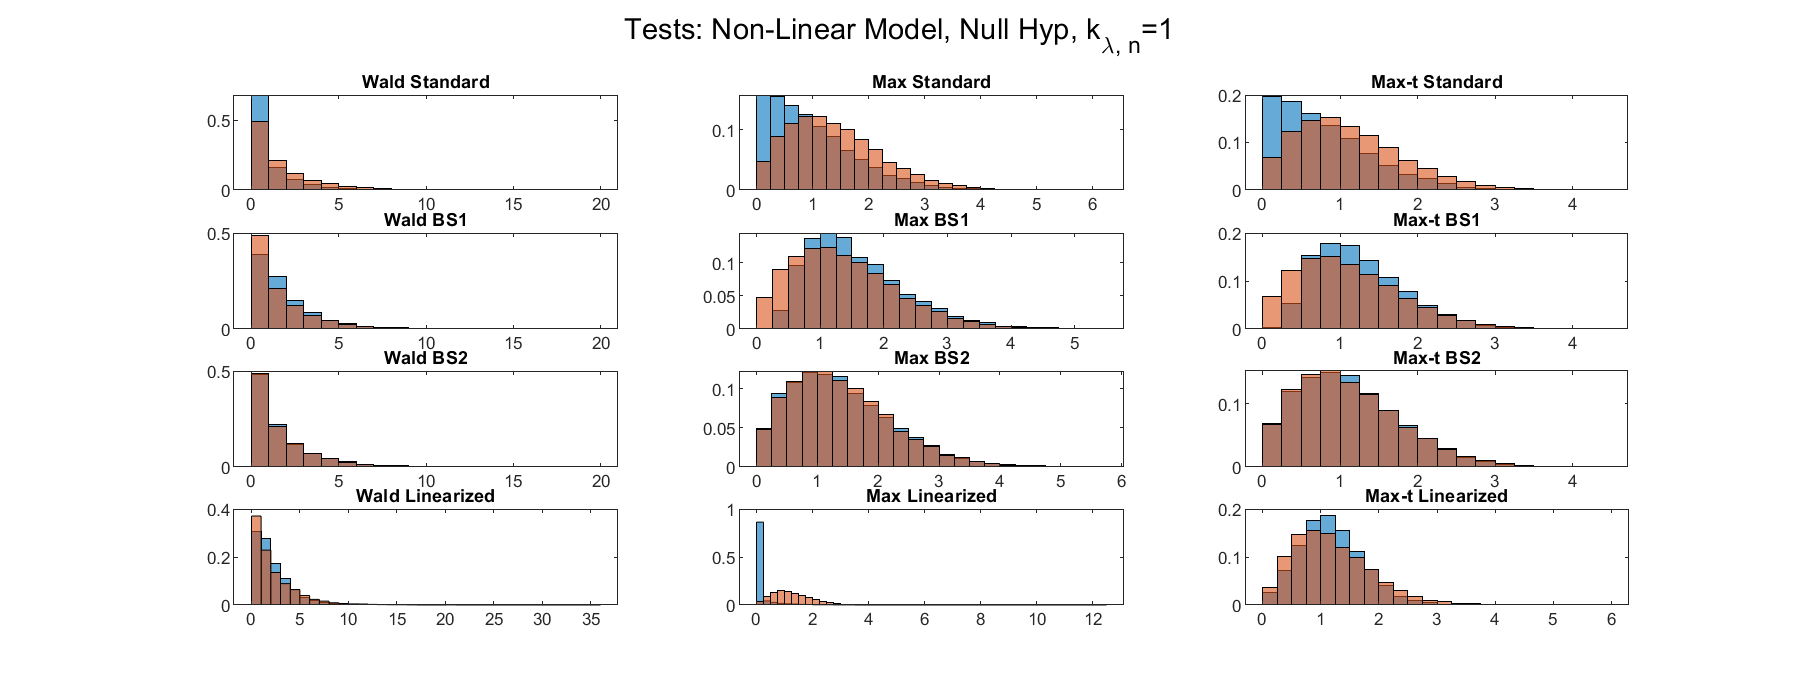
\includegraphics[scale=.5]{./figs/hist_tests_1_dgp2_hyp1_n200_kd1_kl1_b11000_b20_J10000.png}
\end{figure}
\hfill 
\hyperlink{simulation_results_null_table}{\beamergotobutton{Return to table}}
}

\frame{
\frametitle{Simulation Results}
\begin{figure}[H]
\centering
\hspace*{-2cm}
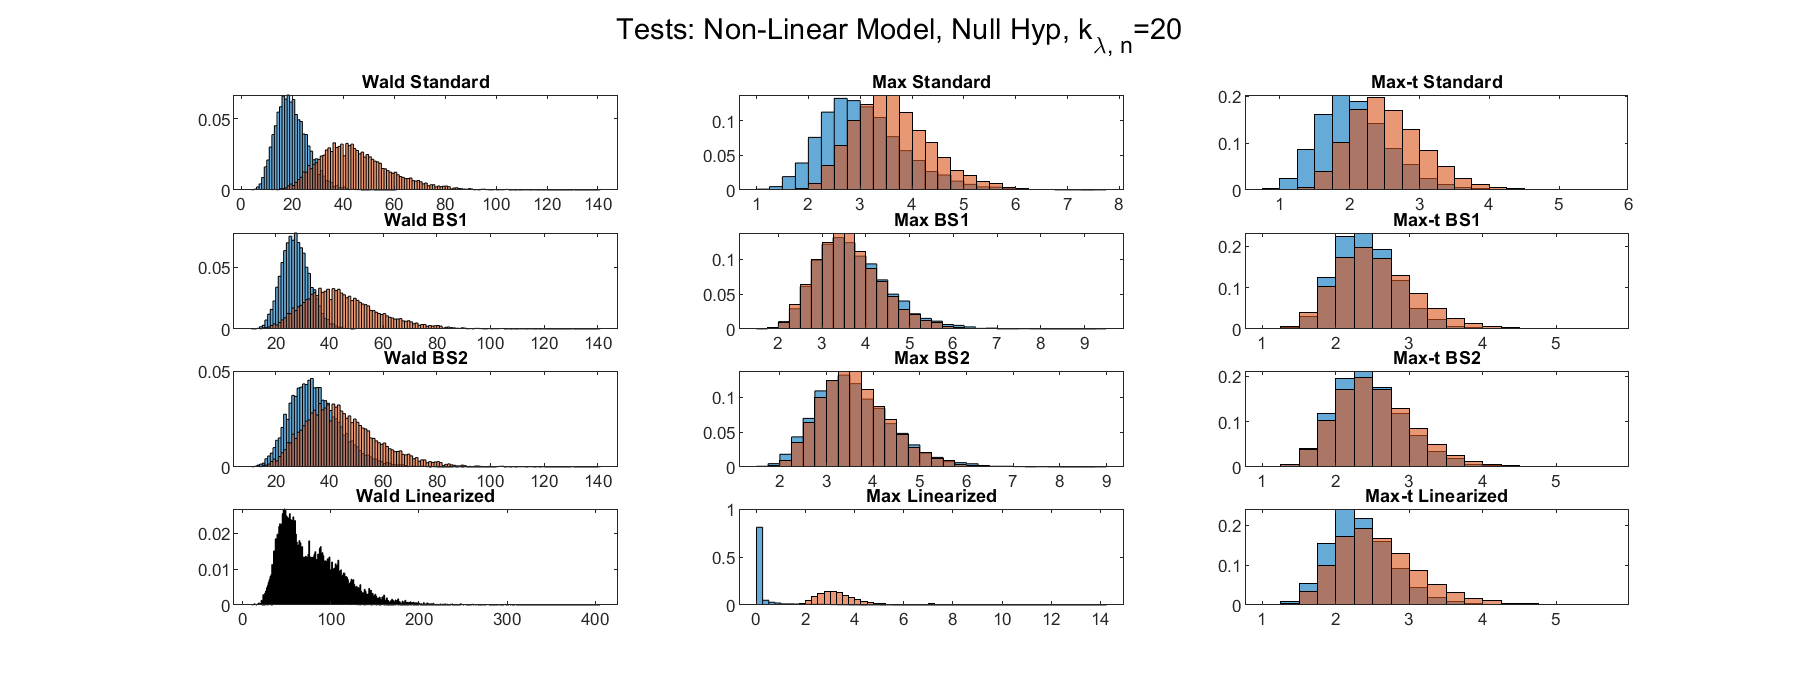
\includegraphics[scale=.5]{./figs/hist_tests_1_dgp2_hyp1_n200_kd1_kl20_b11000_b20_J10000.png}
\end{figure}
\hfill 
\hyperlink{simulation_results_null_table}{\beamergotobutton{Return to table}}
}






\subsection*{Extra Stuff}









\backupend


\end{document}



%%%%%%%%%%%%%%%%%%%%%%%%
%%%%%%%%%%%%%%%%%%%%%%%%
%%%%%%%%%%%%%%%%%%%%%%%%
%%%%%%%%%%%%%%%%%%%%%%%%
%%%%%%%%%%%%%%%%%%%%%%%%
%%%%%%%%%%%%%%%%%%%%%%%%
%%%%%%%%%%%%%%%%%%%%%%%%
%%%%%%%%%%%%%%%%%%%%%%%%
%%%%%%%%%%%%%%%%%%%%%%%%
%%%%%%%%%%%%%%%%%%%%%%%%
%%%%%%%%%%%%%%%%%%%%%%%%
%%%%%%%%%%%%%%%%%%%%%%%%
%%%%%%%%%%%%%%%%%%%%%%%%
%%%%%%%%%%%%%%%%%%%%%%%%
%%%%%%%%%%%%%%%%%%%%%%%%
%%%%%%%%%%%%%%%%%%%%%%%%
%%%%%%%%%%%%%%%%%%%%%%%%
%%%%%%%%%%%%%%%%%%%%%%%%
%%%%%%%%%%%%%%%%%%%%%%%%
%%%%%%%%%%%%%%%%%%%%%%%%
%%%%%%%%%%%%%%%%%%%%%%%%
%%%%%%%%%%%%%%%%%%%%%%%%
%%%%%%%%%%%%%%%%%%%%%%%%
%%%%%%%%%%%%%%%%%%%%%%%%
%%%%%%%%%%%%%%%%%%%%%%%%
%%%%%%%%%%%%%%%%%%%%%%%%
%%%%%%%%%%%%%%%%%%%%%%%%
%%%%%%%%%%%%%%%%%%%%%%%%
%%%%%%%%%%%%%%%%%%%%%%%%
%%%%%%%%%%%%%%%%%%%%%%%%
%%%%%%%%%%%%%%%%%%%%%%%%
%%%%%%%%%%%%%%%%%%%%%%%%
%%%%%%%%%%%%%%%%%%%%%%%%
%%%%%%%%%%%%%%%%%%%%%%%%
%%%%%%%%%%%%%%%%%%%%%%%%
%%%%%%%%%%%%%%%%%%%%%%%%
%%%%%%%%%%%%%%%%%%%%%%%%
%%%%%%%%%%%%%%%%%%%%%%%%
%%%%%%%%%%%%%%%%%%%%%%%%
%%%%%%%%%%%%%%%%%%%%%%%%
%%%%%%%%%%%%%%%%%%%%%%%%
%%%%%%%%%%%%%%%%%%%%%%%%
%%%%%%%%%%%%%%%%%%%%%%%%
%%%%%%%%%%%%%%%%%%%%%%%%
%%%%%%%%%%%%%%%%%%%%%%%%
%%%%%%%%%%%%%%%%%%%%%%%%
%%%%%%%%%%%%%%%%%%%%%%%%
%%%%%%%%%%%%%%%%%%%%%%%%
%%%%%%%%%%%%%%%%%%%%%%%%
%%%%%%%%%%%%%%%%%%%%%%%%
%%%%%%%%%%%%%%%%%%%%%%%%
%%%%%%%%%%%%%%%%%%%%%%%%
%%%%%%%%%%%%%%%%%%%%%%%%
%%%%%%%%%%%%%%%%%%%%%%%%
%%%%%%%%%%%%%%%%%%%%%%%%
%%%%%%%%%%%%%%%%%%%%%%%%
%%%%%%%%%%%%%%%%%%%%%%%%
%%%%%%%%%%%%%%%%%%%%%%%%
%%%%%%%%%%%%%%%%%%%%%%%%
%%%%%%%%%%%%%%%%%%%%%%%%
%%%%%%%%%%%%%%%%%%%%%%%%
%%%%%%%%%%%%%%%%%%%%%%%%
%%%%%%%%%%%%%%%%%%%%%%%%
%%%%%%%%%%%%%%%%%%%%%%%%
%%%%%%%%%%%%%%%%%%%%%%%%
%%%%%%%%%%%%%%%%%%%%%%%%
%%%%%%%%%%%%%%%%%%%%%%%%
%%%%%%%%%%%%%%%%%%%%%%%%
%%%%%%%%%%%%%%%%%%%%%%%%
%%%%%%%%%%%%%%%%%%%%%%%%
%%%%%%%%%%%%%%%%%%%%%%%%
%%%%%%%%%%%%%%%%%%%%%%%%
%%%%%%%%%%%%%%%%%%%%%%%%
%%%%%%%%%%%%%%%%%%%%%%%%
%%%%%%%%%%%%%%%%%%%%%%%%
%%%%%%%%%%%%%%%%%%%%%%%%
%%%%%%%%%%%%%%%%%%%%%%%%
%%%%%%%%%%%%%%%%%%%%%%%%
%%%%%%%%%%%%%%%%%%%%%%%%
%%%%%%%%%%%%%%%%%%%%%%%%
%%%%%%%%%%%%%%%%%%%%%%%%
%%%%%%%%%%%%%%%%%%%%%%%%
%%%%%%%%%%%%%%%%%%%%%%%%
%%%%%%%%%%%%%%%%%%%%%%%%
%%%%%%%%%%%%%%%%%%%%%%%%
%%%%%%%%%%%%%%%%%%%%%%%%
%%%%%%%%%%%%%%%%%%%%%%%%
%%%%%%%%%%%%%%%%%%%%%%%%
%%%%%%%%%%%%%%%%%%%%%%%%
%%%%%%%%%%%%%%%%%%%%%%%%
%%%%%%%%%%%%%%%%%%%%%%%%
%%%%%%%%%%%%%%%%%%%%%%%%
%%%%%%%%%%%%%%%%%%%%%%%%
%%%%%%%%%%%%%%%%%%%%%%%%
%%%%%%%%%%%%%%%%%%%%%%%%
%%%%%%%%%%%%%%%%%%%%%%%%
%%%%%%%%%%%%%%%%%%%%%%%%
%%%%%%%%%%%%%%%%%%%%%%%%
%%%%%%%%%%%%%%%%%%%%%%%%
%%%%%%%%%%%%%%%%%%%%%%%%
%%%%%%%%%%%%%%%%%%%%%%%%
%%%%%%%%%%%%%%%%%%%%%%%%
%%%%%%%%%%%%%%%%%%%%%%%%
%%%%%%%%%%%%%%%%%%%%%%%%
%%%%%%%%%%%%%%%%%%%%%%%%
%%%%%%%%%%%%%%%%%%%%%%%%
%%%%%%%%%%%%%%%%%%%%%%%%
%%%%%%%%%%%%%%%%%%%%%%%%
%%%%%%%%%%%%%%%%%%%%%%%%
%%%%%%%%%%%%%%%%%%%%%%%%
%%%%%%%%%%%%%%%%%%%%%%%%
%%%%%%%%%%%%%%%%%%%%%%%%
%%%%%%%%%%%%%%%%%%%%%%%%
%%%%%%%%%%%%%%%%%%%%%%%%
%%%%%%%%%%%%%%%%%%%%%%%%
%%%%%%%%%%%%%%%%%%%%%%%%
%%%%%%%%%%%%%%%%%%%%%%%%
%%%%%%%%%%%%%%%%%%%%%%%%
%%%%%%%%%%%%%%%%%%%%%%%%
%%%%%%%%%%%%%%%%%%%%%%%%
%%%%%%%%%%%%%%%%%%%%%%%%
%%%%%%%%%%%%%%%%%%%%%%%%
%%%%%%%%%%%%%%%%%%%%%%%%
%%%%%%%%%%%%%%%%%%%%%%%%
%%%%%%%%%%%%%%%%%%%%%%%%
%%%%%%%%%%%%%%%%%%%%%%%%
%%%%%%%%%%%%%%%%%%%%%%%%
%%%%%%%%%%%%%%%%%%%%%%%%
%%%%%%%%%%%%%%%%%%%%%%%%
%%%%%%%%%%%%%%%%%%%%%%%%
%%%%%%%%%%%%%%%%%%%%%%%%
%%%%%%%%%%%%%%%%%%%%%%%%
%%%%%%%%%%%%%%%%%%%%%%%%
%%%%%%%%%%%%%%%%%%%%%%%%
%%%%%%%%%%%%%%%%%%%%%%%%
%%%%%%%%%%%%%%%%%%%%%%%%
%%%%%%%%%%%%%%%%%%%%%%%%
%%%%%%%%%%%%%%%%%%%%%%%%
%%%%%%%%%%%%%%%%%%%%%%%%
%%%%%%%%%%%%%%%%%%%%%%%%
%%%%%%%%%%%%%%%%%%%%%%%%
%%%%%%%%%%%%%%%%%%%%%%%%
%%%%%%%%%%%%%%%%%%%%%%%%
%%%%%%%%%%%%%%%%%%%%%%%%
%%%%%%%%%%%%%%%%%%%%%%%%
%%%%%%%%%%%%%%%%%%%%%%%%
%%%%%%%%%%%%%%%%%%%%%%%%
%%%%%%%%%%%%%%%%%%%%%%%%
%%%%%%%%%%%%%%%%%%%%%%%%
%%%%%%%%%%%%%%%%%%%%%%%%
%%%%%%%%%%%%%%%%%%%%%%%%
%%%%%%%%%%%%%%%%%%%%%%%%
%%%%%%%%%%%%%%%%%%%%%%%%
%%%%%%%%%%%%%%%%%%%%%%%%
%%%%%%%%%%%%%%%%%%%%%%%%
%%%%%%%%%%%%%%%%%%%%%%%%
%%%%%%%%%%%%%%%%%%%%%%%%
%%%%%%%%%%%%%%%%%%%%%%%%
%%%%%%%%%%%%%%%%%%%%%%%%
%%%%%%%%%%%%%%%%%%%%%%%%
%%%%%%%%%%%%%%%%%%%%%%%%
%%%%%%%%%%%%%%%%%%%%%%%%
%%%%%%%%%%%%%%%%%%%%%%%%
%%%%%%%%%%%%%%%%%%%%%%%%
%%%%%%%%%%%%%%%%%%%%%%%%
%%%%%%%%%%%%%%%%%%%%%%%%
%%%%%%%%%%%%%%%%%%%%%%%%
%%%%%%%%%%%%%%%%%%%%%%%%
%%%%%%%%%%%%%%%%%%%%%%%%
%%%%%%%%%%%%%%%%%%%%%%%%
%%%%%%%%%%%%%%%%%%%%%%%%
%%%%%%%%%%%%%%%%%%%%%%%%
%%%%%%%%%%%%%%%%%%%%%%%%
%%%%%%%%%%%%%%%%%%%%%%%%
%%%%%%%%%%%%%%%%%%%%%%%%
%%%%%%%%%%%%%%%%%%%%%%%%
%%%%%%%%%%%%%%%%%%%%%%%%
%%%%%%%%%%%%%%%%%%%%%%%%
%%%%%%%%%%%%%%%%%%%%%%%%
%%%%%%%%%%%%%%%%%%%%%%%%
%%%%%%%%%%%%%%%%%%%%%%%%
%%%%%%%%%%%%%%%%%%%%%%%%
%%%%%%%%%%%%%%%%%%%%%%%%
%%%%%%%%%%%%%%%%%%%%%%%%
%%%%%%%%%%%%%%%%%%%%%%%%
%%%%%%%%%%%%%%%%%%%%%%%%
%%%%%%%%%%%%%%%%%%%%%%%%
%%%%%%%%%%%%%%%%%%%%%%%%
%%%%%%%%%%%%%%%%%%%%%%%%
%%%%%%%%%%%%%%%%%%%%%%%%
%%%%%%%%%%%%%%%%%%%%%%%%
%%%%%%%%%%%%%%%%%%%%%%%%
%%%%%%%%%%%%%%%%%%%%%%%%
%%%%%%%%%%%%%%%%%%%%%%%%
%%%%%%%%%%%%%%%%%%%%%%%%
%%%%%%%%%%%%%%%%%%%%%%%%
%%%%%%%%%%%%%%%%%%%%%%%%
%%%%%%%%%%%%%%%%%%%%%%%%
%%%%%%%%%%%%%%%%%%%%%%%%
%%%%%%%%%%%%%%%%%%%%%%%%
%%%%%%%%%%%%%%%%%%%%%%%%
%%%%%%%%%%%%%%%%%%%%%%%%
%%%%%%%%%%%%%%%%%%%%%%%%
%%%%%%%%%%%%%%%%%%%%%%%%
%%%%%%%%%%%%%%%%%%%%%%%%
%%%%%%%%%%%%%%%%%%%%%%%%
%%%%%%%%%%%%%%%%%%%%%%%%
%%%%%%%%%%%%%%%%%%%%%%%%
%%%%%%%%%%%%%%%%%%%%%%%%
%%%%%%%%%%%%%%%%%%%%%%%%
%%%%%%%%%%%%%%%%%%%%%%%%
%%%%%%%%%%%%%%%%%%%%%%%%
%%%%%%%%%%%%%%%%%%%%%%%%
%%%%%%%%%%%%%%%%%%%%%%%%
%%%%%%%%%%%%%%%%%%%%%%%%
%%%%%%%%%%%%%%%%%%%%%%%%
%%%%%%%%%%%%%%%%%%%%%%%%
%%%%%%%%%%%%%%%%%%%%%%%%
%%%%%%%%%%%%%%%%%%%%%%%%
%%%%%%%%%%%%%%%%%%%%%%%%
%%%%%%%%%%%%%%%%%%%%%%%%
%%%%%%%%%%%%%%%%%%%%%%%%
%%%%%%%%%%%%%%%%%%%%%%%%
%%%%%%%%%%%%%%%%%%%%%%%%
%%%%%%%%%%%%%%%%%%%%%%%%
%%%%%%%%%%%%%%%%%%%%%%%%
%%%%%%%%%%%%%%%%%%%%%%%%
%%%%%%%%%%%%%%%%%%%%%%%%
%%%%%%%%%%%%%%%%%%%%%%%%
%%%%%%%%%%%%%%%%%%%%%%%%
%%%%%%%%%%%%%%%%%%%%%%%%
%%%%%%%%%%%%%%%%%%%%%%%%
%%%%%%%%%%%%%%%%%%%%%%%%
%%%%%%%%%%%%%%%%%%%%%%%%
%%%%%%%%%%%%%%%%%%%%%%%%
%%%%%%%%%%%%%%%%%%%%%%%%
%%%%%%%%%%%%%%%%%%%%%%%%
%%%%%%%%%%%%%%%%%%%%%%%%
%%%%%%%%%%%%%%%%%%%%%%%%
%%%%%%%%%%%%%%%%%%%%%%%%
%%%%%%%%%%%%%%%%%%%%%%%%
%%%%%%%%%%%%%%%%%%%%%%%%
%%%%%%%%%%%%%%%%%%%%%%%%
%%%%%%%%%%%%%%%%%%%%%%%%
%%%%%%%%%%%%%%%%%%%%%%%%
%%%%%%%%%%%%%%%%%%%%%%%%
%%%%%%%%%%%%%%%%%%%%%%%%
%%%%%%%%%%%%%%%%%%%%%%%%
%%%%%%%%%%%%%%%%%%%%%%%%
%%%%%%%%%%%%%%%%%%%%%%%%
%%%%%%%%%%%%%%%%%%%%%%%%
%%%%%%%%%%%%%%%%%%%%%%%%
%%%%%%%%%%%%%%%%%%%%%%%%
%%%%%%%%%%%%%%%%%%%%%%%%
%%%%%%%%%%%%%%%%%%%%%%%%
%%%%%%%%%%%%%%%%%%%%%%%%
%%%%%%%%%%%%%%%%%%%%%%%%
%%%%%%%%%%%%%%%%%%%%%%%%
%%%%%%%%%%%%%%%%%%%%%%%%
%%%%%%%%%%%%%%%%%%%%%%%%
%%%%%%%%%%%%%%%%%%%%%%%%
%%%%%%%%%%%%%%%%%%%%%%%%
%%%%%%%%%%%%%%%%%%%%%%%%
%%%%%%%%%%%%%%%%%%%%%%%%
%%%%%%%%%%%%%%%%%%%%%%%%
%%%%%%%%%%%%%%%%%%%%%%%%
%%%%%%%%%%%%%%%%%%%%%%%%
%%%%%%%%%%%%%%%%%%%%%%%%
%%%%%%%%%%%%%%%%%%%%%%%%
%%%%%%%%%%%%%%%%%%%%%%%%
%%%%%%%%%%%%%%%%%%%%%%%%
%%%%%%%%%%%%%%%%%%%%%%%%
%%%%%%%%%%%%%%%%%%%%%%%%
%%%%%%%%%%%%%%%%%%%%%%%%
%%%%%%%%%%%%%%%%%%%%%%%%
%%%%%%%%%%%%%%%%%%%%%%%%
%%%%%%%%%%%%%%%%%%%%%%%%
%%%%%%%%%%%%%%%%%%%%%%%%
%%%%%%%%%%%%%%%%%%%%%%%%
%%%%%%%%%%%%%%%%%%%%%%%%
%%%%%%%%%%%%%%%%%%%%%%%%
%%%%%%%%%%%%%%%%%%%%%%%%
%%%%%%%%%%%%%%%%%%%%%%%%
%%%%%%%%%%%%%%%%%%%%%%%%
%%%%%%%%%%%%%%%%%%%%%%%%
%%%%%%%%%%%%%%%%%%%%%%%%
%%%%%%%%%%%%%%%%%%%%%%%%
%%%%%%%%%%%%%%%%%%%%%%%%
%%%%%%%%%%%%%%%%%%%%%%%%
%%%%%%%%%%%%%%%%%%%%%%%%
%%%%%%%%%%%%%%%%%%%%%%%%
%%%%%%%%%%%%%%%%%%%%%%%%
%%%%%%%%%%%%%%%%%%%%%%%%
%%%%%%%%%%%%%%%%%%%%%%%%
%%%%%%%%%%%%%%%%%%%%%%%%
%%%%%%%%%%%%%%%%%%%%%%%%
%%%%%%%%%%%%%%%%%%%%%%%%
%%%%%%%%%%%%%%%%%%%%%%%%
%%%%%%%%%%%%%%%%%%%%%%%%
%%%%%%%%%%%%%%%%%%%%%%%%
%%%%%%%%%%%%%%%%%%%%%%%%
%%%%%%%%%%%%%%%%%%%%%%%%
%%%%%%%%%%%%%%%%%%%%%%%%
%%%%%%%%%%%%%%%%%%%%%%%%
%%%%%%%%%%%%%%%%%%%%%%%%
%%%%%%%%%%%%%%%%%%%%%%%%
%%%%%%%%%%%%%%%%%%%%%%%%
%%%%%%%%%%%%%%%%%%%%%%%%
%%%%%%%%%%%%%%%%%%%%%%%%
%%%%%%%%%%%%%%%%%%%%%%%%
%%%%%%%%%%%%%%%%%%%%%%%%
%%%%%%%%%%%%%%%%%%%%%%%%
%%%%%%%%%%%%%%%%%%%%%%%%
%%%%%%%%%%%%%%%%%%%%%%%%
%%%%%%%%%%%%%%%%%%%%%%%%
%%%%%%%%%%%%%%%%%%%%%%%%
%%%%%%%%%%%%%%%%%%%%%%%%
%%%%%%%%%%%%%%%%%%%%%%%%
%%%%%%%%%%%%%%%%%%%%%%%%
%%%%%%%%%%%%%%%%%%%%%%%%
%%%%%%%%%%%%%%%%%%%%%%%%
%%%%%%%%%%%%%%%%%%%%%%%%
%%%%%%%%%%%%%%%%%%%%%%%%
%%%%%%%%%%%%%%%%%%%%%%%%
%%%%%%%%%%%%%%%%%%%%%%%%
%%%%%%%%%%%%%%%%%%%%%%%%
%%%%%%%%%%%%%%%%%%%%%%%%
%%%%%%%%%%%%%%%%%%%%%%%%
%%%%%%%%%%%%%%%%%%%%%%%%
%%%%%%%%%%%%%%%%%%%%%%%%
%%%%%%%%%%%%%%%%%%%%%%%%
%%%%%%%%%%%%%%%%%%%%%%%%
%%%%%%%%%%%%%%%%%%%%%%%%
%%%%%%%%%%%%%%%%%%%%%%%%
%%%%%%%%%%%%%%%%%%%%%%%%
%%%%%%%%%%%%%%%%%%%%%%%%
%%%%%%%%%%%%%%%%%%%%%%%%
%%%%%%%%%%%%%%%%%%%%%%%%
%%%%%%%%%%%%%%%%%%%%%%%%
%%%%%%%%%%%%%%%%%%%%%%%%
%%%%%%%%%%%%%%%%%%%%%%%%
%%%%%%%%%%%%%%%%%%%%%%%%
%%%%%%%%%%%%%%%%%%%%%%%%
%%%%%%%%%%%%%%%%%%%%%%%%
%%%%%%%%%%%%%%%%%%%%%%%%
%%%%%%%%%%%%%%%%%%%%%%%%
%%%%%%%%%%%%%%%%%%%%%%%%
%%%%%%%%%%%%%%%%%%%%%%%%
%%%%%%%%%%%%%%%%%%%%%%%%
%%%%%%%%%%%%%%%%%%%%%%%%
%%%%%%%%%%%%%%%%%%%%%%%%
%%%%%%%%%%%%%%%%%%%%%%%%
%%%%%%%%%%%%%%%%%%%%%%%%
%%%%%%%%%%%%%%%%%%%%%%%%
%%%%%%%%%%%%%%%%%%%%%%%%
%%%%%%%%%%%%%%%%%%%%%%%%
%%%%%%%%%%%%%%%%%%%%%%%%
%%%%%%%%%%%%%%%%%%%%%%%%
%%%%%%%%%%%%%%%%%%%%%%%%
%%%%%%%%%%%%%%%%%%%%%%%%
%%%%%%%%%%%%%%%%%%%%%%%%
%%%%%%%%%%%%%%%%%%%%%%%%
%%%%%%%%%%%%%%%%%%%%%%%%
%%%%%%%%%%%%%%%%%%%%%%%%
%%%%%%%%%%%%%%%%%%%%%%%%
%%%%%%%%%%%%%%%%%%%%%%%%
%%%%%%%%%%%%%%%%%%%%%%%%
%%%%%%%%%%%%%%%%%%%%%%%%
%%%%%%%%%%%%%%%%%%%%%%%%
%%%%%%%%%%%%%%%%%%%%%%%%
%%%%%%%%%%%%%%%%%%%%%%%%
%%%%%%%%%%%%%%%%%%%%%%%%
%%%%%%%%%%%%%%%%%%%%%%%%
%%%%%%%%%%%%%%%%%%%%%%%%
%%%%%%%%%%%%%%%%%%%%%%%%
%%%%%%%%%%%%%%%%%%%%%%%%
%%%%%%%%%%%%%%%%%%%%%%%%
%%%%%%%%%%%%%%%%%%%%%%%%
%%%%%%%%%%%%%%%%%%%%%%%%
%%%%%%%%%%%%%%%%%%%%%%%%
%%%%%%%%%%%%%%%%%%%%%%%%
%%%%%%%%%%%%%%%%%%%%%%%%
%%%%%%%%%%%%%%%%%%%%%%%%
%%%%%%%%%%%%%%%%%%%%%%%%
%%%%%%%%%%%%%%%%%%%%%%%%
%%%%%%%%%%%%%%%%%%%%%%%%
%%%%%%%%%%%%%%%%%%%%%%%%
%%%%%%%%%%%%%%%%%%%%%%%%
%%%%%%%%%%%%%%%%%%%%%%%%
%%%%%%%%%%%%%%%%%%%%%%%%
%%%%%%%%%%%%%%%%%%%%%%%%
%%%%%%%%%%%%%%%%%%%%%%%%
%%%%%%%%%%%%%%%%%%%%%%%%
%%%%%%%%%%%%%%%%%%%%%%%%
%%%%%%%%%%%%%%%%%%%%%%%%
%%%%%%%%%%%%%%%%%%%%%%%%
%%%%%%%%%%%%%%%%%%%%%%%%
%%%%%%%%%%%%%%%%%%%%%%%%
%%%%%%%%%%%%%%%%%%%%%%%%
%%%%%%%%%%%%%%%%%%%%%%%%
%%%%%%%%%%%%%%%%%%%%%%%%
%%%%%%%%%%%%%%%%%%%%%%%%
%%%%%%%%%%%%%%%%%%%%%%%%
%%%%%%%%%%%%%%%%%%%%%%%%
%%%%%%%%%%%%%%%%%%%%%%%%
%%%%%%%%%%%%%%%%%%%%%%%%
%%%%%%%%%%%%%%%%%%%%%%%%
%%%%%%%%%%%%%%%%%%%%%%%%
%%%%%%%%%%%%%%%%%%%%%%%%
%%%%%%%%%%%%%%%%%%%%%%%%
%%%%%%%%%%%%%%%%%%%%%%%%
%%%%%%%%%%%%%%%%%%%%%%%%
%%%%%%%%%%%%%%%%%%%%%%%%
%%%%%%%%%%%%%%%%%%%%%%%%
%%%%%%%%%%%%%%%%%%%%%%%%
%%%%%%%%%%%%%%%%%%%%%%%%
%%%%%%%%%%%%%%%%%%%%%%%%
%%%%%%%%%%%%%%%%%%%%%%%%
%%%%%%%%%%%%%%%%%%%%%%%%
%%%%%%%%%%%%%%%%%%%%%%%%
%%%%%%%%%%%%%%%%%%%%%%%%
%%%%%%%%%%%%%%%%%%%%%%%%
%%%%%%%%%%%%%%%%%%%%%%%%
%%%%%%%%%%%%%%%%%%%%%%%%
%%%%%%%%%%%%%%%%%%%%%%%%
%%%%%%%%%%%%%%%%%%%%%%%%
%%%%%%%%%%%%%%%%%%%%%%%%
%%%%%%%%%%%%%%%%%%%%%%%%
%%%%%%%%%%%%%%%%%%%%%%%%
%%%%%%%%%%%%%%%%%%%%%%%%
%%%%%%%%%%%%%%%%%%%%%%%%
%%%%%%%%%%%%%%%%%%%%%%%%
%%%%%%%%%%%%%%%%%%%%%%%%
%%%%%%%%%%%%%%%%%%%%%%%%
%%%%%%%%%%%%%%%%%%%%%%%%
%%%%%%%%%%%%%%%%%%%%%%%%
%%%%%%%%%%%%%%%%%%%%%%%%
%%%%%%%%%%%%%%%%%%%%%%%%
%%%%%%%%%%%%%%%%%%%%%%%%
%%%%%%%%%%%%%%%%%%%%%%%%
%%%%%%%%%%%%%%%%%%%%%%%%
%%%%%%%%%%%%%%%%%%%%%%%%
%%%%%%%%%%%%%%%%%%%%%%%%
%%%%%%%%%%%%%%%%%%%%%%%%
%%%%%%%%%%%%%%%%%%%%%%%%
%%%%%%%%%%%%%%%%%%%%%%%%





\frame{
\frametitle{Overview - Identification Robust Max Correlation Test}
\begin{itemize}
\setlength\itemsep{.25cm}
\item It is known that parameter identification failure causes nonstandard estimator distributions
\item \highlight{Point 1}: What happens to other tests based on estimated models when parameters are near identification failure?
\begin{itemize}
\item the nonstandardness propagates to our test statistic for serial correlation.
\item Ignoring identification failure can lead to distorted inference:
\end{itemize}
%\input{./sim_observations/ARMA/arma_garch_size_distortion.tex}
 \begin{table}[H] 
 \small 
 \centering 
\begin{tabular}{ccc} 
% \hline 
 & Traditional Test & Our Robust Test \\ 
 \hline 
 $(\alpha=0.05)$ & 0.096 &  0.050 \\ 
 \hline 
% & & \\
\multicolumn{3}{c}{ \tiny Rejection Frequencies, ARMA-GARCH, $T=100$, Weak Id, Max Correlation Test} \\ 
% \multicolumn{3}{c}{ $T=100$, $J=500$ } \\ 
\end{tabular}
 \end{table}

\item \highlight{Point 2}: What do we do when standard methods fail?
\begin{itemize}
\item We provide a test that leads to correct inference
\end{itemize}
%\item We develop a bootstrap procedure for inference depending upon whether identification failure is present or not
%\item Inference based on our procedure is robust to the behavior resulting from identification failure
\end{itemize}
}




% \frame{
% \frametitle{Why do we care about Serial Correlation?}
% Put further questions in an appendix slide - talk about the ARMA model there (e.g. Valentin's question)
% }




\frame{
\frametitle{Identification?}
Consider the ARMA(1,1) model:
\begin{equation*}
y_{t} = \gamma y_{t-1} + \e_{t} - \pi \e_{t-1}
\end{equation*}
Imagine $y_{t}$ carries no dependence.
\begin{itemize}
\item Typically we assume this means $\gamma = 0$, $\pi = 0$.
\item But in general $\gamma = \pi \ne 0$ $\Rightarrow$ no dependence.
\end{itemize}

\begin{itemize}
\item The general case is called the `Common Roots Problem.'  

\item We typically assume this problem away because it prevents identification of $\gamma$ and $\pi$.

\item However, there are common situations in which this may be an issue.
\end{itemize}
}


\frame[label = identification_is_a_real_issue]{
\frametitle{Identification?}
\begin{itemize}
\item \cite{Taylor2005}
\begin{itemize}
\item low levels of dependence in returns can be exploited
\item trading rule based on ARMA(1,1) model of returns
\end{itemize}

 \begin{table}[H] 
 \tiny 
 \centering 
\begin{tabular}{|c|c|c|c|c|c|c|} % c|} 
\multicolumn{7}{c}{ VWRETD, monthly data, ARMA, Unknown Id } \\ 
%\multicolumn{7}{c}{ ARMA, Unknown Id } \\ 
 \hline 
 &  1  &  2  &  3  &  4  &  5  &  6  \\ % &  7    \\ 
 \hline 
 Start Date &  31-Jul-1962 &  31-Jul-1962 &  31-Oct-1978 &  31-Jul-1962 &  31-Jan-1995 &  31-Oct-1978  \\ % &  29-Jan-1988 \\ 
 End Date &  30-Dec-1994 &  29-Sep-1978 &  30-Dec-1994 &  30-Dec-2005 &  30-Dec-2005 &  30-Dec-2005  \\ % &  30-Dec-2005 \\ 
 n &   389  &   194  &   194  &   521  &   131  &   326   \\ % &   215  \\ 
 \hline
 \hline
  &     &     &     &     &     &      \\ % &     \\ 
 $\hat{\beta}_{n}$ &  0.075 &  0.096 &  0.034 &  0.070 &  0.088 &  0.036  \\ % &  0.051 \\ 
 $\hat{se}$ &  (0.914) &  (0.735) &  (0.244) &  (0.637) &  (0.817) &  (0.237)  \\ % &  (0.623) \\ 
 \hline 
\end{tabular}
 \end{table}


\item Set $\gamma = \beta + \pi$ to focus on identification of $\pi$.
\hfill 
\hyperlink{ARMA_0}{\beamergotobutton{ARMA}}

\item $\pi$ is not identified when $\beta = 0$.

\item We don't know if $\beta = 0$ or not.

\item Statistically, $\beta$ appears close to 0, and even being close can be problematic.
\end{itemize}
}






\frame[label = ARMA_beta_hat_id1]{
\frametitle{Identification Failure for the Parameters}
Identification failure leads to non-standard distributions:

\hspace*{-1cm}
% \begin{tabular}{cc}
% 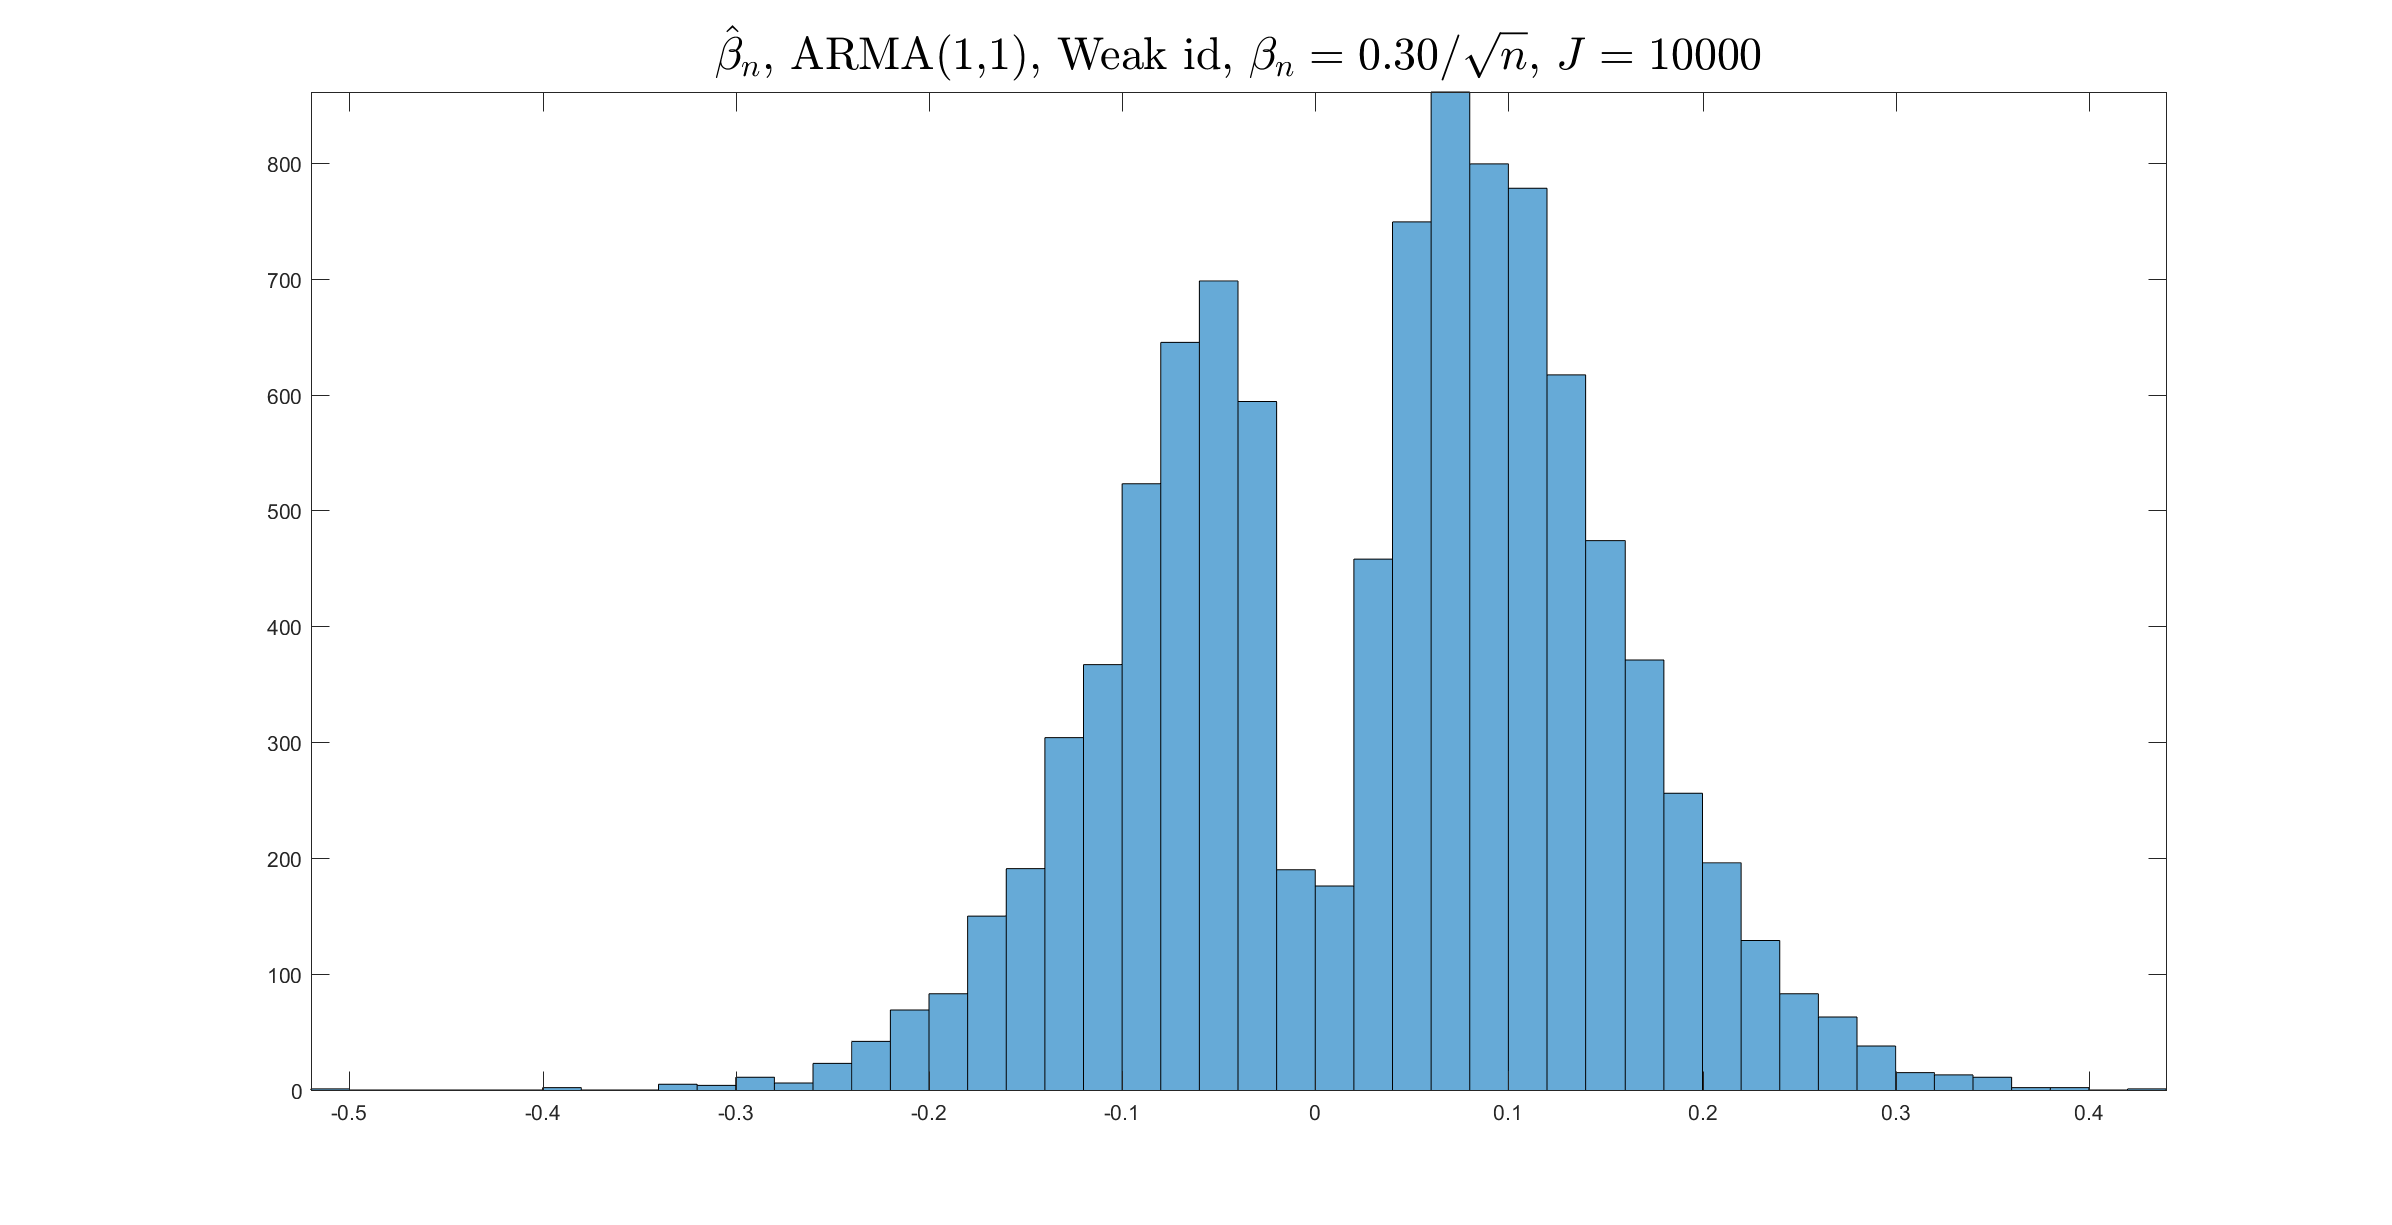
\includegraphics[scale=.16]{./fig/ARMA_beta_hat_id1_J10000.png} &
% 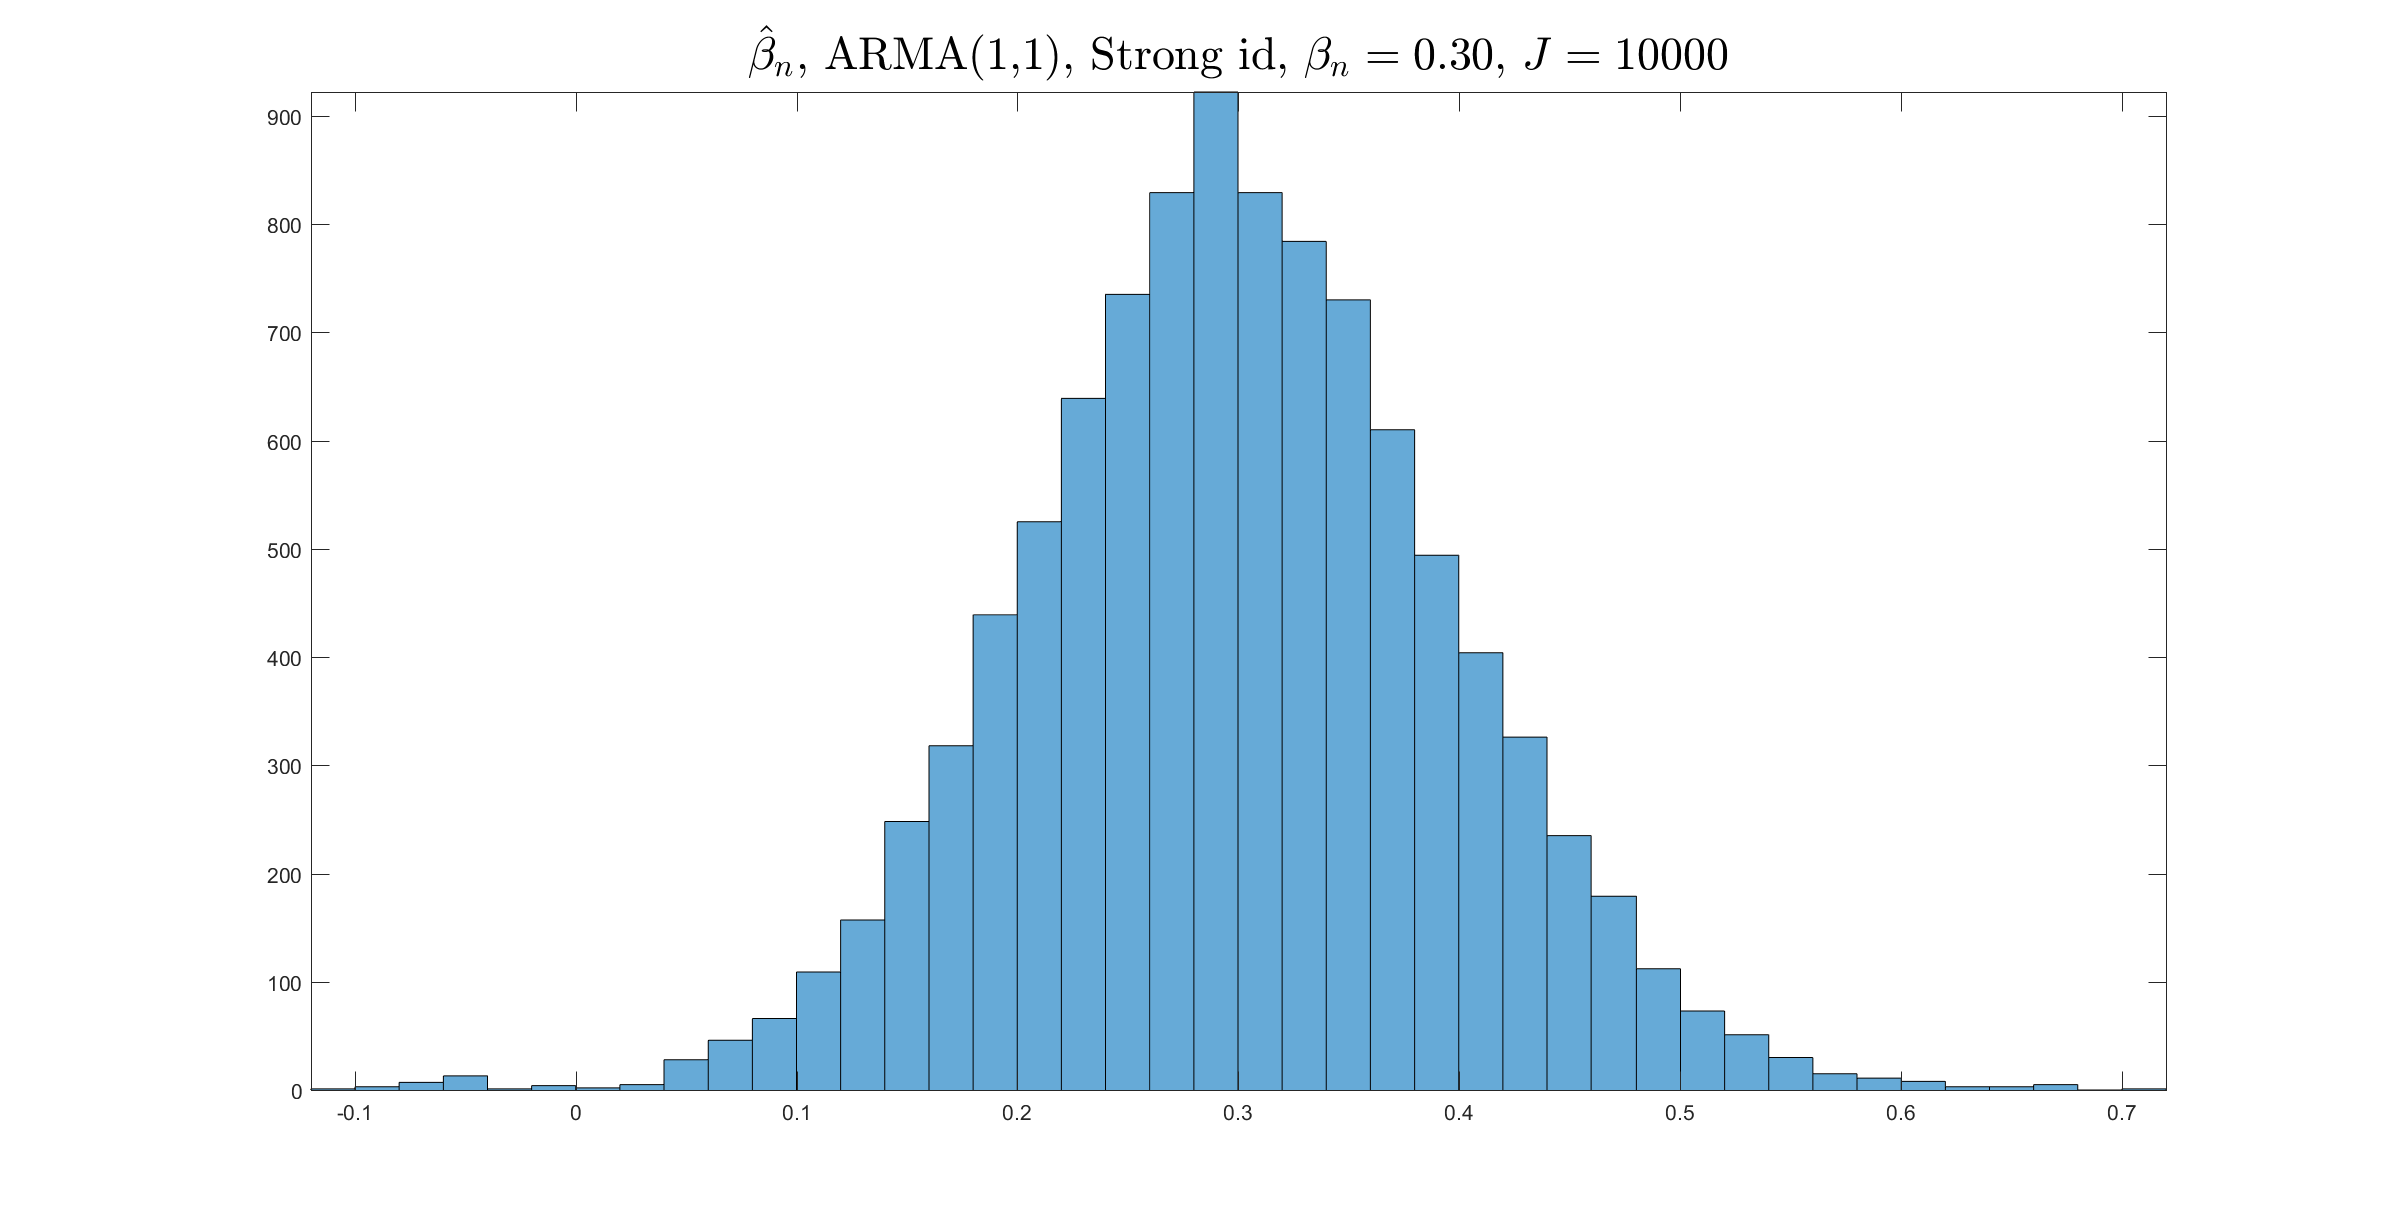
\includegraphics[scale=.16]{./fig/ARMA_beta_hat_id2_J10000.png} \\
% Close to Unidentified & Identified
% \end{tabular}
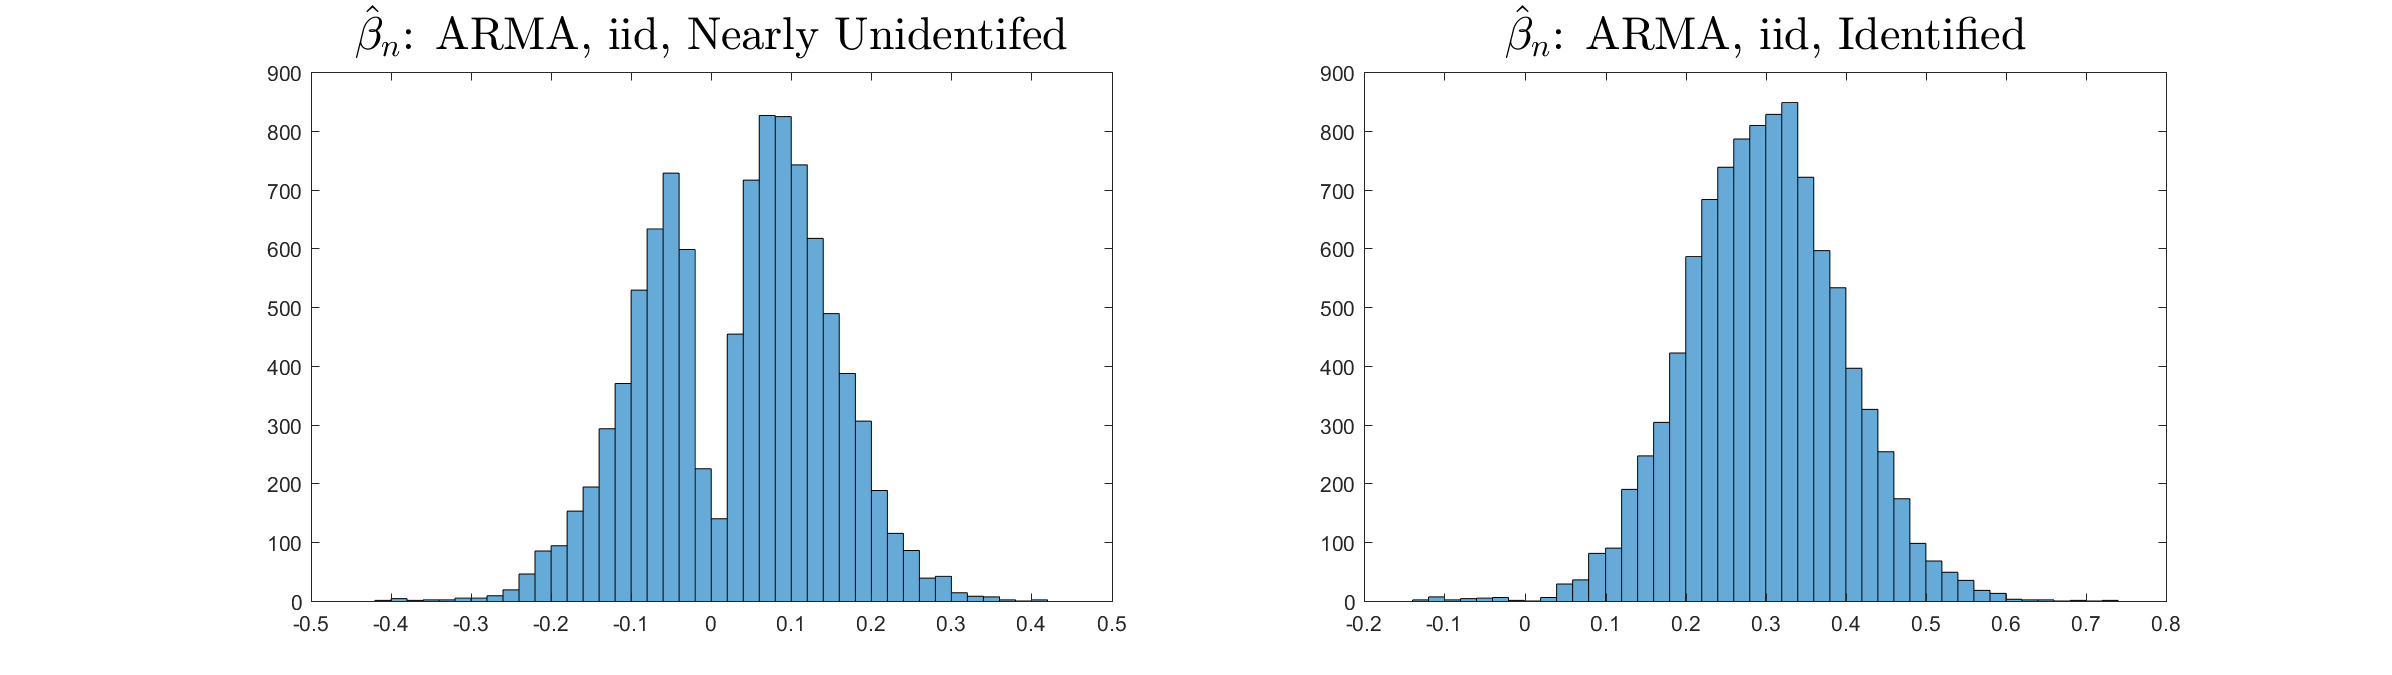
\includegraphics[scale=.35]{../fig/beta_hat_i1.png}

\vspace*{.25cm}
\begin{itemize}
\item 
$\Rightarrow$ Non-standard Inference!
\hfill 
%\hyperlink{STAR_beta_hat_id1}{\beamergotobutton{STAR(1) $\hat{\beta}_{n}$}}
\hyperlink{ARMA_beta_hat_id0}{\beamergotobutton{ARMA(1,1) $\hat{\beta}_{n}$, non-id}}

%\vspace*{.25cm}
%\item Current inference relies on calculation of distributions \citep{AndrewsPloberger1996,AndrewsCheng2012,Cheng2015}

%\item We will bootstrap
\end{itemize}
}



\frame[label = ARMA_use_motivation]{
\frametitle{Identification Failure in our Test}
\begin{itemize}
\item Imagine we want to use the ARMA model to inform a trading rule \citep{Taylor2005}.  

\hfill
\hyperlink{id_robust_models}{\beamergotobutton{Other Uses}}

\vspace*{1cm}
\item We want to know if the ARMA model adequately describes our data.

\vspace*{1cm}
\item Test for serial correlation in the residuals: 
\begin{itemize}
\item If we detect serial correlation in the residuals, then our model must not be characterizing some dependence.  
\end{itemize}
\end{itemize}
}









\frame[label = test_first_order_expansion]{
\frametitle{Identification Failure in our Test}
\begin{itemize}
\setlength\itemsep{.25cm}
\item Note: \textit{We are not testing the parameter values!}
\item But our test does use the residuals from the estimated model
\item We must account for the influence of model estimation on our test statistic:
%Proving the limiting distribution of and bootstrapping the test statistic involves an expansion that includes these estimator distributions:
\begin{align*}
\hat{\Tc}_n \equiv \hat{\Tc}_n(\hat{\theta}_n) 
= \hat{\Tc}_n(\theta_{n}^*) + \underbrace{\sqrt{n}(\hat{\theta}_n - \theta_{n}^*)}_{\text{\highlight{Non-standard}}} \hat{\D}_n + o_{p}(1) 
\end{align*}

\item `Non-standardness' can be felt beyond inference on the parameter values!

\end{itemize}

\vfill \hfill
\hyperlink{related_literature}{\beamergotobutton{Related Literature}}
}


\frame{
\frametitle{Identification Failure in our Test}
\hspace*{-1.2cm}
% \begin{tabular}{ll}
% 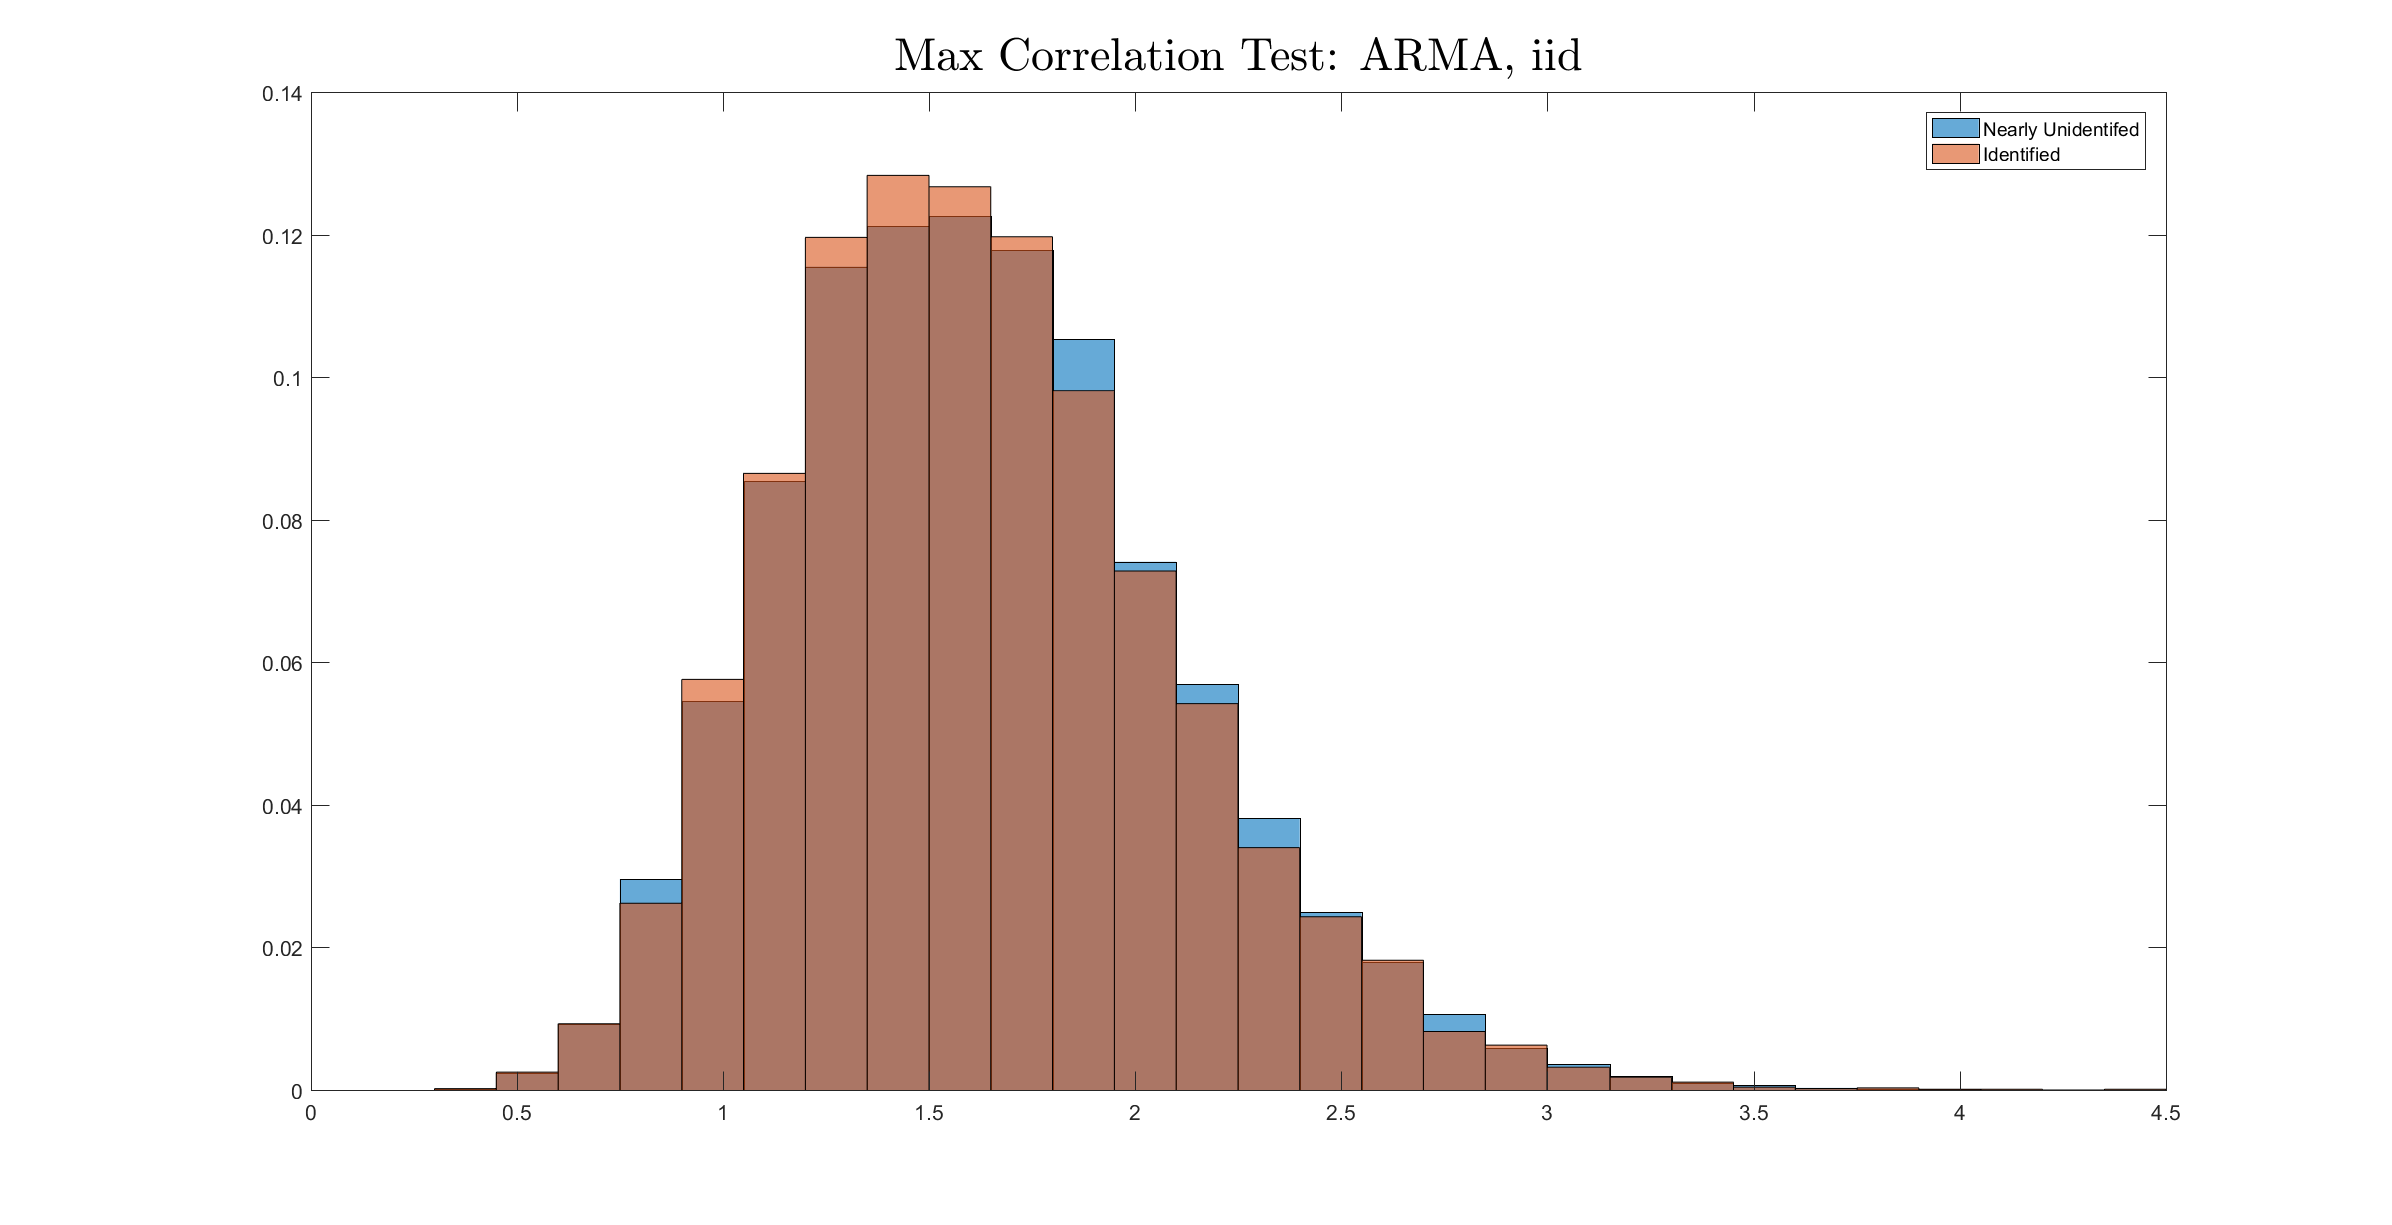
\includegraphics[scale=.18]{../fig/MC_hat_i1_Ln2.png} &
% \hspace*{-1.5cm}
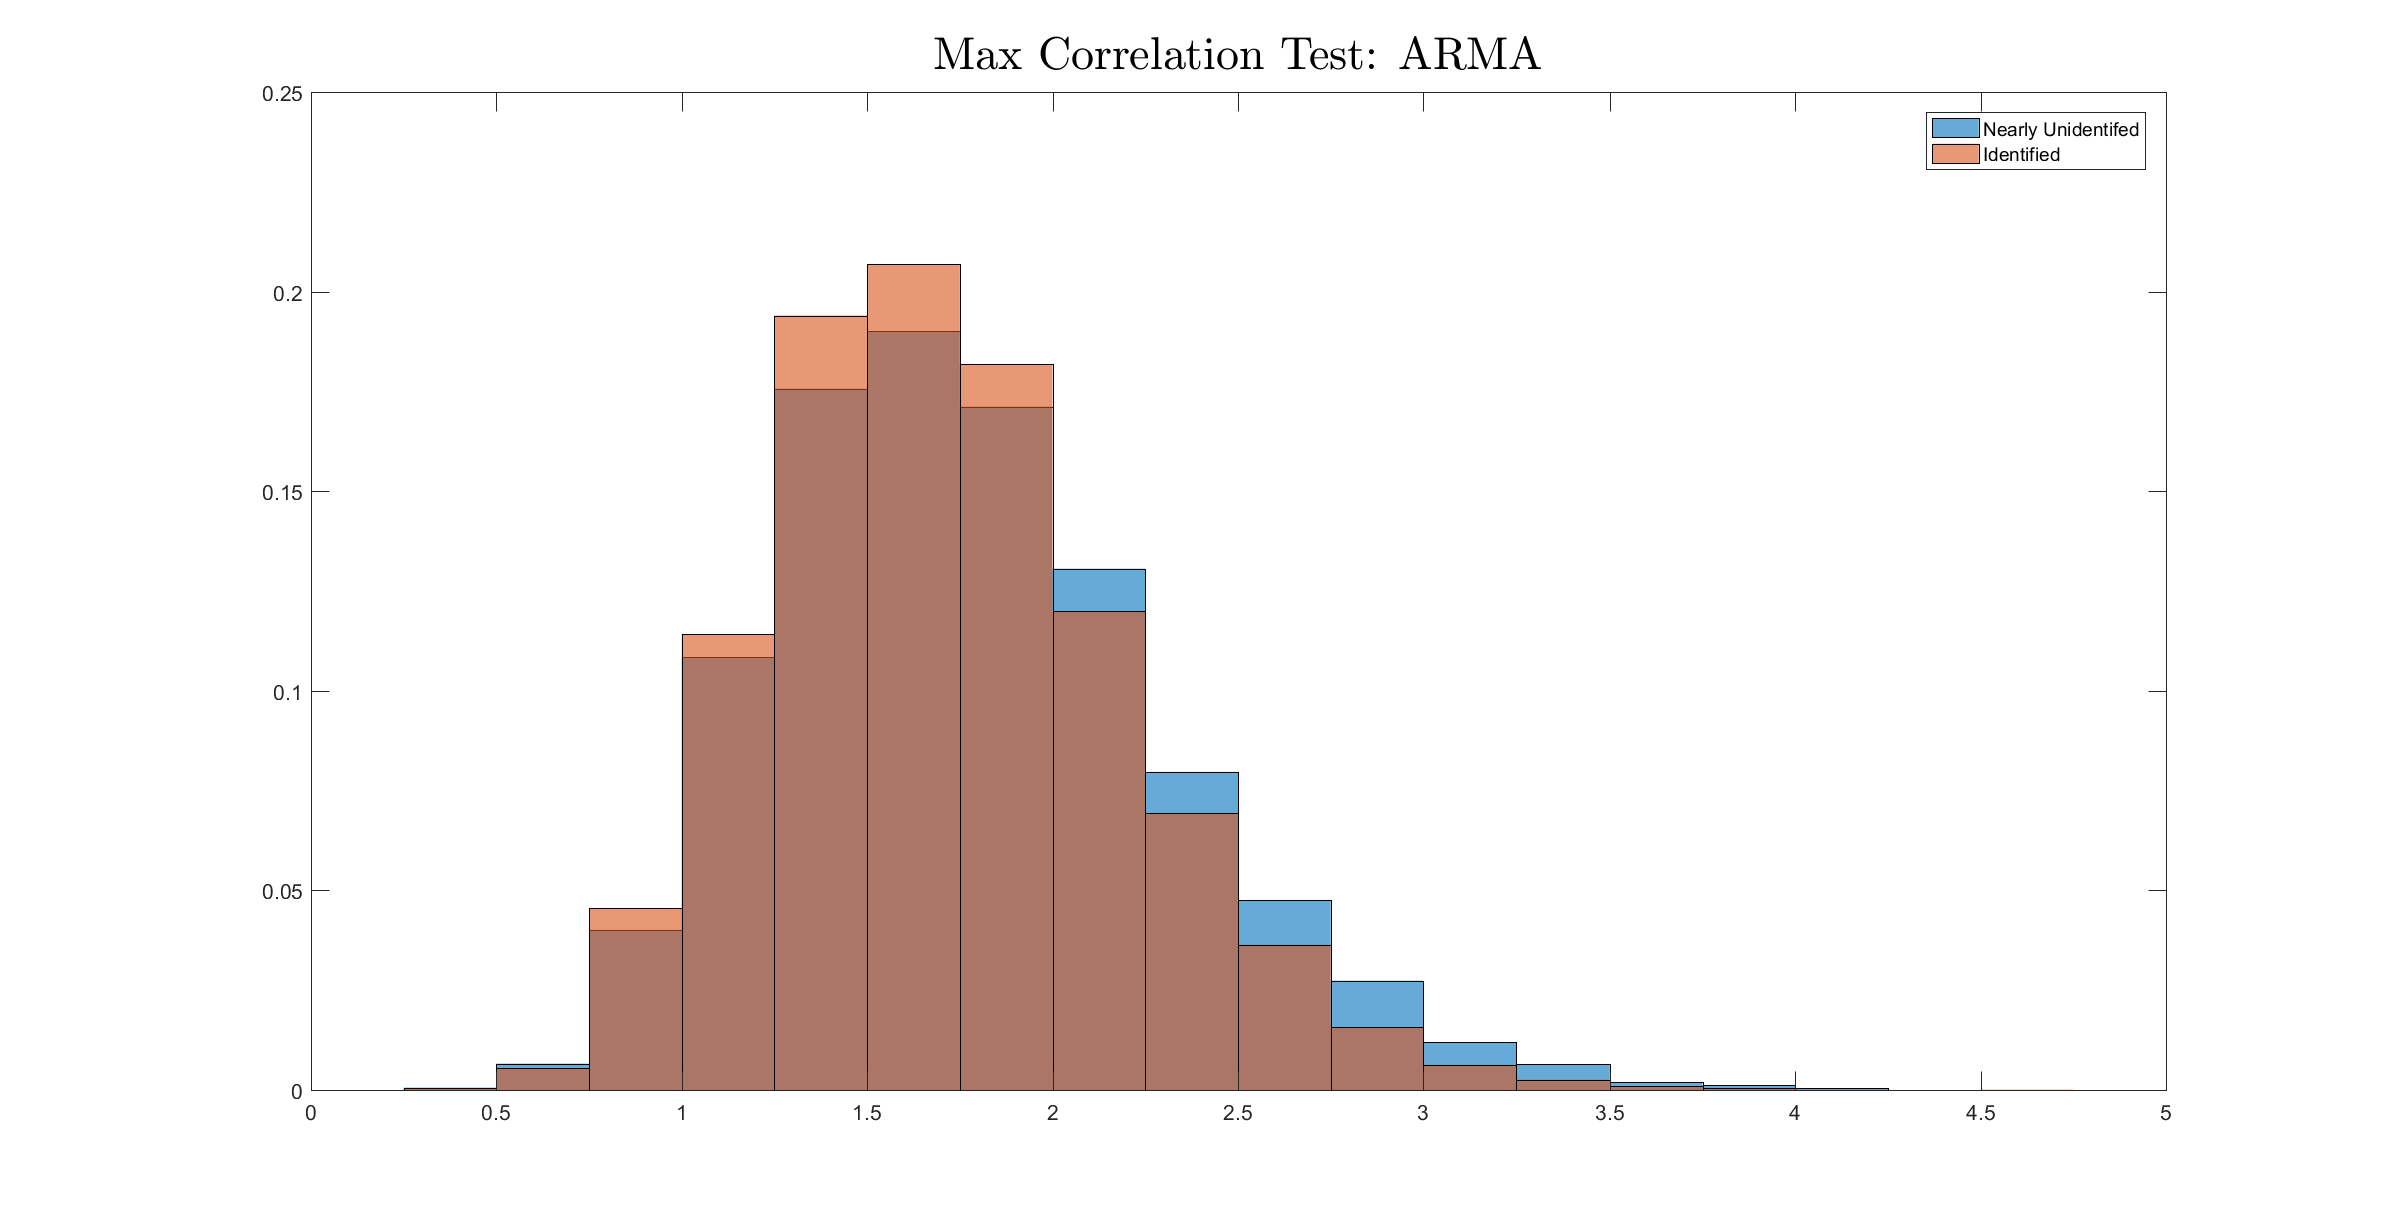
\includegraphics[scale=.35]{../fig/MC_hat_i3_Ln2.png}
% \end{tabular}
\vfill
\begin{center}
\textit{We show how to correctly conduct inference.}
\end{center}
}










%%%%%%%%%%%%%%%%%%%%%%%%%%%
%%%%%%%%%%%%%%%%%%%%%%%%%%%
%%%%%%%%%%%%%%%%%%%%%%%%%%%
%%%%%%%%%%%%%%%%%%%%%%%%%%%
%%%%%%%%%%%%%%%%%%%%%%%%%%%

% \section{Identification Framework}






%%%%%%%%%%%%%%%%%%%%%%%%%%%
%%%%%%%%%%%%%%%%%%%%%%%%%%%
%%%%%%%%%%%%%%%%%%%%%%%%%%%
%%%%%%%%%%%%%%%%%%%%%%%%%%%
%%%%%%%%%%%%%%%%%%%%%%%%%%%

% \section{Max Tests}










% % % % % % % % % % % % % % % % %
% % % % % % % % % % % % % % % % %
% % % % % % % % % % % % % % % % %
% % % % % % % % % % % % % % % % %
% % % % % % % % % % % % % % % % %
% % % % % % % % % % % % % % % % %
% % % % % % % % % % % % % % % % %
% % % % % % % % % % % % % % % % %

\section{White Noise Test}
\addtocounter{framenumber}{-1}
\frame{
\frametitle{Outline}
\tableofcontents[ 
	currentsection, 
    %currentsubsection, 
    hideothersubsections, 
    %sectionstyle=show/hide, 
    %subsectionstyle=show/shaded, 
    ] 
}



\frame[label = white_noise_test_recap]{
\frametitle{White Noise Test}
\begin{itemize}%[<+->] %[<+-| alert@+>]
\setlength\itemsep{.25cm}
\item model with \textbf{known} source of identification failure: 
\hfill 
\hyperlink{ARMA_0}{\beamergotobutton{ARMA}}
\hspace*{.25cm}
\hyperlink{STAR_0}{\beamergotobutton{STAR}}

\[ \e_t(\theta), \quad \e_t(\theta_n) \equiv \e_t\]

\item We want to test if $\{\e_t\}$ is a white noise process:
\begin{equation*}
H_0: \rho(h) = 0 \ \forall h \in \N \ \text{ vs. } \ H_{A}: \rho(h) \ne 0 \ \text{ for some } h \in \N 
\end{equation*}
where $\rho(h) = E(\e_t \e_{t-h}) / E(\e_t^2)$.

\item using the sample max correlation statistic 
\[\hat{\Tc}_n = \max_{1\le h \le \Le_n} |\sqrt{n} \hat{\rho}_n(h)|\]
\end{itemize}

\vfill
\hfill 
\hyperlink{max_tests_explanation_slide}{\beamergotobutton{Max Tests?}}

%\hfill 
%\hyperlink{slide_for_Valentin}{\beamergotobutton{Why not use Taylor?}}

\hfill 
\hyperlink{max_test_comments}{\beamergotobutton{Comments}}
}



%\subsection{Critical Values}

\frame[label = critical_values_short_slide]{
\frametitle{Critical Values}

Recall 2 distributions 
\hyperlink{Test_stat_theorem}{\beamergotobutton{Theory}}

\begin{itemize}
\item We don't know which is correct - must bootstrap each individually
\hyperlink{bootstrap_procedure}{\beamergotobutton{ Bootstrap Procedure}}

\item 2 different critical values - How to combine them?

\item ICS - Use data to determine if parameter is identified
\hyperlink{robust_cvs}{\beamergotobutton{ICS Details}}

\begin{itemize}
\item if so, then use identified cv
\item if not, take the larger of the 2 cvs
\end{itemize}
\end{itemize}


Test Properties
\begin{itemize}
\item Correct Asymptotic Size {\small (largest rejection probability under the null is $\alpha$)}
\hyperlink{theory_correct_asym_size}{\beamergotobutton{Theory}}

\item Consistent {\small (Under Alternative, probability of rejecting null $\to 1$)}
\hyperlink{theory_test_consistency}{\beamergotobutton{Theory}}
\end{itemize}

This is good, but how does it do in practice?

%\vfill \hfill \hyperlink{critical_values_short_slide}{\beamergotobutton{Return to CV slide}}
}



%%%%%%%%%%%%%%%%%%
%%%%%%%%%%%%%%%%%%
%%%%%%%%%%%%%%%%%%
%%%%%%%%%%%%%%%%%%
%%%%%%%%%%%%%%%%%%
%%%%%%%%%%%%%%%%%%
%%%%%%%%%%%%%%%%%%
%%%%%%%%%%%%%%%%%%
%%%%%%%%%%%%%%%%%%
%%%%%%%%%%%%%%%%%%
%%%%%%%%%%%%%%%%%%
%%%%%%%%%%%%%%%%%%







%%%%%%%%%%%%%%%%%%%%%%%%%%%%%%%%%%%%%
%%%%%%%%%%%%%%%%%%%%%%%%%%%%%%%%%%%%%
%%%%%%%%%%%%%%%%%%%%%%%%%%%%%%%%%%%%%
%%%%%%%%%%%%%%%%%%%%%%%%%%%%%%%%%%%%%
%%%%%%%%%%%%%%%%%%%%%%%%%%%%%%%%%%%%%
%%%%%%%%%%%%%%%%%%%%%%%%%%%%%%%%%%%%%
%%%%%%%%%%%%%%%%%%%%%%%%%%%%%%%%%%%%%
%%%%%%%%%%%%%%%%%%%%%%%%%%%%%%%%%%%%%
%%%%%%%%%%%%%%%%%%%%%%%%%%%%%%%%%%%%%
%%%%%%%%%%%%%%%%%%%%%%%%%%%%%%%%%%%%%
%%%%%%%%%%%%%%%%%%%%%%%%%%%%%%%%%%%%%
%%%%%%%%%%%%%%%%%%%%%%%%%%%%%%%%%%%%%
%%%%%%%%%%%%%%%%%%%%%%%%%%%%%%%%%%%%%
%%%%%%%%%%%%%%%%%%%%%%%%%%%%%%%%%%%%%
%%%%%%%%%%%%%%%%%%%%%%%%%%%%%%%%%%%%%



\section{Simulations}

\addtocounter{framenumber}{-1}
\frame{
\frametitle{Outline}
\tableofcontents[ 
	currentsection, 
    %currentsubsection, 
    hideothersubsections, 
    %sectionstyle=show/hide, 
    %subsectionstyle=show/shaded, 
    ] 
}



\frame{
\frametitle{Summary of Simulation Results}
%Summary of Simulation Results
\begin{itemize}
\item Benchmark: Infeasible Tests - We know the true value of the unidentified parameters
\item Real World: Feasible Tests - Must evaluate over a grid of nuisance parameters
\end{itemize}

\begin{itemize}
\setlength{\itemsep}{10pt}
%\item ARMA(1,1) % and STAR(1)
\item Good size and power for infeasible tests

\item %ARMA(1,1) model 
When truth is near identification failure: 

\begin{itemize}
\setlength{\itemsep}{10pt}
\item Tests ignoring the identification issue are over-sized

\item Robust tests control size well

\item Current issue: Nuisance parameters $\Rightarrow$ low empirical power in  \highlight{feasible} tests...
\end{itemize}
\end{itemize}

}


\frame[label = sim_model_setup]{
\frametitle{Monte Carlo Simulations}
\begin{table}[H]
\centering
\begin{tabular}[H]{ll}
%STAR(1): & $y_{t} = \frac{\highlight{\beta_n} y_{t-1}}{1+ \exp({\color{blue} -10}(y_{t-1} - \highlight{0}))} + \highlight{.5} y_{t-1} + \e_{t}$ \\
% & \\
%{\small Misspecified STAR(2):} & $y_{t} = \frac{\highlight{\beta_n} y_{t-1}}{1+ \exp(-10(y_{t-1} - \highlight{0}))} + \highlight{.5} y_{t-1} + {\color{cyan} \frac{.15}{\sqrt{n}}} y_{t-2} + \e_{t}$ \\
% & \\
ARMA(1,1): & $y_{t} = (\highlight{\beta_n} + \highlight{.5})y_{t-1} + \e_{t} - \highlight{.5} \e_{t-1}$
\end{tabular}
\end{table}

with $\beta_n \in \{0, \highlight{.3 / \sqrt{n}}, \highlight{.3} \}$.
Let $\nu_{t} \sim$ iid $N(0,1)$.  % Then for $\e_{t}$:

\begin{table}[H]
\centering
\begin{tabular}[H]{ll}
\multicolumn{2}{c}{$H_0$} \\
\hline
iid:          & $\e_{t} = \nu_{t}$ \\
GARCH(1,1):   & $\e_{t} = \sigma_t \nu_{t}$, \\
              & $\sigma_t^2 = 1 + .3 \e_{t-1}^2 + .6 \sigma_{t-1}^2$ \\
% Bilinear:     & $\e_{t} = .5 \e_{t-1} \nu_{t-1} +  \nu_{t}$ \\
\hline
\end{tabular}
\end{table}
\vspace*{-.25cm}
\begin{table}[H]
\centering
\begin{tabular}[H]{ll}
\multicolumn{2}{c}{$H_A$} \\
\hline
AR(2):   & $\e_{t} = .5 \e_{t-2} + \nu_{t}$ \\
%MA(1):   & $\e_{t} = .5 \nu_{t-1} + \nu_{t}$ \\
MA(10):  & $\e_{t} = .5 \nu_{t-10} + \nu_{t}$ \\
\hline
\end{tabular}
\begin{tabular}[H]{ll}
\multicolumn{2}{c}{$H_A$} \\
\hline
MA(21):  & $\e_{t} = .5 \nu_{t-21} + \nu_{t}$ \\
MA(50):  & $\e_{t} = .5 \nu_{t-50} + \nu_{t}$ \\
%MA(100):  & $\e_{t} = .5 \nu_{t-100} + \nu_{t}$ \\
\hline
\end{tabular}
\end{table}
\vfill \hfill \hyperlink{sim_details}{\beamergotobutton{Simulation Details}}
}



\frame{
\frametitle{Monte Carlo Simulations}
Today, I discuss tests based on 
\begin{itemize}
%\item $LF$ 
\item $ICS$: data driven identification category selection
\item $S$: ignoring identification failure
%\item $NoX$: Ignore model estimation/residuals  
\end{itemize}
for the following tests
\begin{itemize}
\item (MC): Max Correlation Test 
\item (LBQ): \pcite{Hong1996} Standardized Ljung-Box Q test,
\item (CvM): \pcite{Shao2011} Cram{\'e}r von Mises Test, 
\item (supLM): \pcite{NankervisSavin2010} representation of \pcite{AndrewsPloberger1996} sup-LM test
\end{itemize}
%\vfill \hfill \hyperlink{sim_model_setup}{\beamergotobutton{Return to Simulation Setup}}
}




% \frame[label = STAR_sims_0]{
% \frametitle{Simulations - Initial Observations}
% \begin{itemize}
% \item Initial Observations:
% \begin{itemize}
% %\item NoX performs poorly, as expected
% \item LF based tests tend to be overly conservative when the truth is strong identification 
% \item LF performs well when truth is near identification failure.
% %\hyperlink{star_sim_LF}{\beamergotobutton{LF}}
% \item In general, ICS based tests perform well
% \end{itemize}
% \end{itemize}
% }

%\frame{
%\frametitle{Simulations - Initial Observations}
%\input{./sim_observations/NoX.tex}
%}



%
%
%
%
%
%
%


\frame[label = ARMA_sims]{
\frametitle{ARMA Simulations}
\begin{itemize}
\item Size ($H_{0}$ true):
\begin{itemize}
% \item Shrinkage is not noticeable

\item iid, GARCH errors: 
\begin{itemize}
\item ICS controls size well 
% \hyperlink{arma_garch_strong_Ln5}{\beamergotobutton{GARCH}}
\item MC ICS statistics are close to nominal for all id truths 
\end{itemize}

\item Truth near identification failure: Size distortions are noticeable for MC,LBQ,sup LM - S based statistics

% \item CvM tends to be overly conservative

% \item bilinear errors:
% \begin{itemize}
% \item near identification failure: MC ICS is close to nominal at low lags, and size distortions appear at higher lags
% \item strong identification: all tests are overly conservative
% \end{itemize}

\end{itemize}

%\vspace{.3cm}
\item Infeasible Power ($H_{0}$ false):
\begin{itemize}
\item ICS based tests comparable to S based tests for all id cases

\item AR(2): MC tests have moderately larger rejection frequencies

\item MA(10): MC and LBQ have large rf, sup LM and CvM are very low
% \hyperlink{arma_ma10_weak_Ln10}{\beamergotobutton{MA(10), weak id}}
% \hyperlink{arma_ma10_strong_Ln10}{\beamergotobutton{MA(10), strong id}}
\end{itemize}

\item Feasible Power ($H_{0}$ false, accounting for nuisance parameters): 
\begin{itemize}
\item near identification failure: ICS rejections are low, nontrivial for MC, LBQ
\item strong identification: ICS, S are comparable
\end{itemize}

\end{itemize}
\hfill \hyperlink{STAR_sims}{\beamergotobutton{STAR sims}}
}



\frame[label = ARMA_sims_T100]{
\frametitle{ARMA Simulations}
 \begin{table}[H] 
 \tiny 
 \centering 
\begin{tabular}{|c|c|c||c|c|c|c|} 
\multicolumn{7}{c}{ Rejection Frequencies: Robust Tests, Identified } \\ 
\multicolumn{7}{c}{ ARMA, $\alpha = 0.05$, $T=100$, $\beta = 0.300$, $J=500$ } \\ 
% \multicolumn{7}{c}{ $T=100$, $\beta = 0.300$, $J=500$ } \\ 
  \multicolumn{1}{c}{ } & \multicolumn{2}{c}{ $H_{0}$ True} & \multicolumn{4}{c}{ $H_{0}$ False} \\ 
  \multicolumn{1}{c}{ } & \multicolumn{2}{c}{ Infeasible } & \multicolumn{2}{c}{ Infeasible } & \multicolumn{2}{c}{ Feasible} \\ 
 \hline 
% & iid, $\Le_n=5$ & GARCH(1,1), $\Le_n=5$ & AR(2), $\Le_n=5$ & MA(10), $\Le_n=10$ & AR(2), $\Le_n=5$ & MA(10), $\Le_n=10$   \\ 
 & iid & GARCH(1,1) & AR(2) & MA(10) & AR(2) & MA(10)  \\ 
 \hline 
 MC ICS &  0.0460 &  0.0300 &  0.5580 &  0.7600 &  0.5120 &  0.7180 \\ 
 LBQ ICS &  0.0400 &  0.0420 &  0.5180 &  0.5420 &  0.4740 &  0.4780 \\ 
 sup LM ICS &  0.0240 &  0.0500 &  0.5040 &  0.0620 & 0.4560 &  0.0460 \\ 
 CvM ICS &  0.0140 &  0.0240 &  0.4060 &  0.0300 &  0.0040 &  0.0060 \\ 
 \hline 
% MC LF &  0.0140 &  0.0120 &  0.0900 &  0.3660  &  0.5120 &  0.7180 \\ 
% LBQ LF &  0.0100 &  0.0140 &  0.0900 &  0.1420 &  0.4740 &  0.4780 \\ 
% sup LM LF &  0.0080 &  0.0240 &  0.0680 &  0.0160 &  0.4560 &  0.0460 \\ 
% CvM LF &  0.0020 &  0.0060 &  0.0320 &  0.0080 &  0.0040 &  0.0060 \\ 
 MC S &  0.0520 &  0.0340 & & & 0.5820 &  0.7640  \\ % 0.5760 &  0.7640 \\ 
 LBQ S &  0.0400 &  0.0480 & & & 0.5360 &  0.5540  \\ % 0.5220 &  0.5120 \\ 
 sup LM S &  0.0240 &  0.0540 & & & 0.5180 &  0.0620  \\ % 0.5020 &  0.0560 \\ 
 CvM S &  0.0160 &  0.0260 & & & 0.4080 &  0.0340 \\ % 0.0160 &  0.0060 \\ 
% MC NoX &  0.0260 &  0.0100 &  0.8640 &  0.7840 &  0.8340 &  0.7840 \\ 
% LBQ NoX &  0.0200 &  0.0080 &  0.7120 &  0.5180 &  0.6900 &  0.5420 \\ 
% sup LM NoX &  0.0180 &  0.0120 &  0.6200 &  0.0440 &  0.6080 &  0.0560 \\ 
% CvM NoX &  0.0100 &  0.0040 &  0.4940 &  0.0200 &  0.0000 &  0.0000 \\ 
% MC W &  0.0140 &  0.0160 &  0.0900 &  0.3680 &  0.6280 &  0.9300 \\ 
% LBQ W &  0.0100 &  0.0160 &  0.0920 &  0.1440 &  0.6260 &  0.8820 \\ 
% sup LM W &  0.0100 &  0.0320 &  0.0680 &  0.0160 &  0.6280 &  0.9300 \\ 
% CvM W &  0.0040 &  0.0140 &  0.0320 &  0.0080 &  0.6280 &  0.9300 \\ 
 \hline 
\end{tabular}
 \end{table}





\vspace*{-.5cm}
 \begin{table}[H] 
 \tiny 
 \centering 
\begin{tabular}{|c|c|c||c|c|c|c|} 
\multicolumn{7}{c}{ Rejection Frequencies: Robust Tests, Nearly Unidentified } \\ 
\multicolumn{7}{c}{ ARMA, $\alpha = 0.05$, $T=100$, $\beta = 0.030$, $J=500$ } \\ 
% \multicolumn{5}{c}{ $T=100$, $\beta = 0.030$, $J=500$ } \\ 
  \multicolumn{1}{c}{ } & \multicolumn{2}{c}{ $H_{0}$ True} & \multicolumn{4}{c}{ $H_{0}$ False} \\ 
  \multicolumn{1}{c}{ } & \multicolumn{2}{c}{ Infeasible } & \multicolumn{2}{c}{ Infeasible } & \multicolumn{2}{c}{ Feasible} \\ 
 \hline 
% & iid, $\Le_n=5$ & GARCH(1,1), $\Le_n=5$ & AR(2), $\Le_n=5$ & MA(10), $\Le_n=10$   \\ 
 & iid & GARCH(1,1) & AR(2) & MA(10) & AR(2) & MA(10)  \\ 
 & $\Le_n=5$ & $\Le_n=5$ & $\Le_n=5$ & $\Le_n=10$ & $\Le_n=5$ & $\Le_n=10$   \\ 
 \hline 
 MC ICS &  0.0520 &  0.0500 &  0.8900 &  0.8120 & 0.5160 &  0.1508 \\ 
 LBQ ICS &  0.0320 &  0.0360 &  0.8540 &  0.6280 & 0.4680 &  0.1111  \\ 
 sup LM ICS &  0.0140 &  0.0380 &  0.8460 &  0.0420 & 0.4540 &  0.0119  \\ 
 CvM ICS &  0.0040 &  0.0080 &  0.8660 &  0.0140 & 0.0080 &  0.0000  \\ 
 \hline 
% MC LF &  0.0520 &  0.0460 &  0.7640 &  0.7960 \\ 
% LBQ LF &  0.0280 &  0.0280 &  0.7220 &  0.5840 \\ 
% sup LM LF &  0.0140 &  0.0300 &  0.6800 &  0.0360 \\ 
% CvM LF &  0.0040 &  0.0060 &  0.6680 &  0.0060 \\ 
 MC S &  0.0860 &  0.0960 & & &  0.8980 &  0.8460  \\ 
 LBQ S &  0.0760 &  0.0700 & & &  0.8760 &  0.7340  \\ 
 sup LM S &  0.0880 &  0.0900 & & &  0.8720 &  0.1100  \\ 
 CvM S &  0.0480 &  0.0460 & & &  0.8840 &  0.1180  \\ 
% \hline 
% MC NoX &  0.0260 &  0.0180 &  0.8140 &  0.8020 \\ 
% LBQ NoX &  0.0160 &  0.0020 &  0.7040 &  0.5600 \\ 
% sup LM NoX &  0.0080 &  0.0000 &  0.6460 &  0.0180 \\ 
% CvM NoX &  0.0020 &  0.0000 &  0.5560 &  0.0140 \\ 
% MC W &  0.0560 &  0.0560 &  0.7780 &  0.8020 \\ 
% LBQ W &  0.0340 &  0.0340 &  0.7420 &  0.5980 \\ 
% sup LM W &  0.0160 &  0.0580 &  0.6980 &  0.0520 \\ 
% CvM W &  0.0040 &  0.0180 &  0.6960 &  0.0100 \\ 
 \hline 
\end{tabular}
 \end{table}

% MC ICS &   \\ 
% LBQ ICS &   \\ 
% sup LM ICS &   \\ 
% CvM ICS &   \\ 
% MC LF &  0.5160 &  0.1508 \\ 
% LBQ LF &  0.4680 &  0.1111 \\ 
% sup LM LF &  0.4540 &  0.0119 \\ 
% CvM LF &  0.0080 &  0.0000 \\ 
% MC S &  0.8240 &  0.8492 \\ 
% LBQ S &  0.7540 &  0.6627 \\ 
% sup LM S &  0.7340 &  0.0714 \\ 
% CvM S &  0.0120 &  0.0079 \\ 
% MC NoX &  0.7640 &  0.8175 \\ 
% LBQ NoX &  0.6220 &  0.5595 \\ 
% sup LM NoX &  0.5820 &  0.0437 \\ 
% CvM NoX &  0.0000 &  0.0000 \\ 
% MC W &  0.6580 &  0.1865 \\ 
% LBQ W &  0.6360 &  0.1786 \\ 
% sup LM W &  0.6580 &  0.1865 \\ 
% CvM W &  0.6580 &  0.1865 \\ 

\vspace*{-.75cm}
\hfill
\hyperlink{ARMA_sims_T500}{\beamergotobutton{ARMA Sims, T=500}}
}



\addtocounter{framenumber}{-1}
\frame[label = ARMA_sims_T100]{
\frametitle{ARMA Simulations}
 \begin{table}[H] 
 \tiny 
 \centering 
\begin{tabular}{|c|c|c||c|c|c|c|} 
\multicolumn{7}{c}{ Rejection Frequencies: Robust Tests, \highlight{Identified} } \\ 
\multicolumn{7}{c}{ ARMA, $\alpha = 0.05$, $T=100$, $\beta = 0.300$, $J=500$ } \\ 
% \multicolumn{7}{c}{ $T=100$, $\beta = 0.300$, $J=500$ } \\ 
  \multicolumn{1}{c}{ } & \multicolumn{2}{c}{ $H_{0}$ True} & \multicolumn{4}{c}{ $H_{0}$ False} \\ 
  \multicolumn{1}{c}{ } & \multicolumn{2}{c}{ Infeasible } & \multicolumn{2}{c}{ Infeasible } & \multicolumn{2}{c}{ Feasible} \\ 
 \hline 
% & iid, $\Le_n=5$ & GARCH(1,1), $\Le_n=5$ & AR(2), $\Le_n=5$ & MA(10), $\Le_n=10$ & AR(2), $\Le_n=5$ & MA(10), $\Le_n=10$   \\ 
 & iid & GARCH(1,1) & AR(2) & MA(10) & AR(2) & MA(10)  \\ 
 \hline 
 MC ICS &  \highlight{0.0460} &  \highlight{0.0300} &  0.5580 &  0.7600 &  0.5120 &  0.7180 \\ 
 LBQ ICS &  0.0400 &  0.0420 &  0.5180 &  0.5420 &  0.4740 &  0.4780 \\ 
 sup LM ICS &  0.0240 &  0.0500 &  0.5040 &  0.0620 & 0.4560 &  0.0460 \\ 
 CvM ICS &  0.0140 &  0.0240 &  0.4060 &  0.0300 &  0.0040 &  0.0060 \\ 
 \hline 
 MC S &  \highlight{0.0520} &  \highlight{0.0340} & & & 0.5820 &  0.7640  \\ % 0.5760 &  0.7640 \\ 
 LBQ S &  0.0400 &  0.0480 & & & 0.5360 &  0.5540  \\ % 0.5220 &  0.5120 \\ 
 sup LM S &  0.0240 &  0.0540 & & & 0.5180 &  0.0620  \\ % 0.5020 &  0.0560 \\ 
 CvM S &  0.0160 &  0.0260 & & & 0.4080 &  0.0340 \\ % 0.0160 &  0.0060 \\ 
 \hline 
\end{tabular}
 \end{table}





\vspace*{-.5cm}
 \begin{table}[H] 
 \tiny 
 \centering 
\begin{tabular}{|c|c|c||c|c|c|c|} 
\multicolumn{7}{c}{ Rejection Frequencies: Robust Tests, Nearly Unidentified } \\ 
\multicolumn{7}{c}{ ARMA, $\alpha = 0.05$, $T=100$, $\beta = 0.030$, $J=500$ } \\ 
% \multicolumn{5}{c}{ $T=100$, $\beta = 0.030$, $J=500$ } \\ 
  \multicolumn{1}{c}{ } & \multicolumn{2}{c}{ $H_{0}$ True} & \multicolumn{4}{c}{ $H_{0}$ False} \\ 
  \multicolumn{1}{c}{ } & \multicolumn{2}{c}{ Infeasible } & \multicolumn{2}{c}{ Infeasible } & \multicolumn{2}{c}{ Feasible} \\ 
 \hline 
% & iid, $\Le_n=5$ & GARCH(1,1), $\Le_n=5$ & AR(2), $\Le_n=5$ & MA(10), $\Le_n=10$   \\ 
 & iid & GARCH(1,1) & AR(2) & MA(10) & AR(2) & MA(10)  \\ 
 & $\Le_n=5$ & $\Le_n=5$ & $\Le_n=5$ & $\Le_n=10$ & $\Le_n=5$ & $\Le_n=10$   \\ 
 \hline 
 MC ICS &  0.0520 &  0.0500 &  0.8900 &  0.8120 & 0.5160 &  0.1508 \\ 
 LBQ ICS &  0.0320 &  0.0360 &  0.8540 &  0.6280 & 0.4680 &  0.1111  \\ 
 sup LM ICS &  0.0140 &  0.0380 &  0.8460 &  0.0420 & 0.4540 &  0.0119  \\ 
 CvM ICS &  0.0040 &  0.0080 &  0.8660 &  0.0140 & 0.0080 &  0.0000  \\ 
 \hline 
% MC LF &  0.0520 &  0.0460 &  0.7640 &  0.7960 \\ 
% LBQ LF &  0.0280 &  0.0280 &  0.7220 &  0.5840 \\ 
% sup LM LF &  0.0140 &  0.0300 &  0.6800 &  0.0360 \\ 
% CvM LF &  0.0040 &  0.0060 &  0.6680 &  0.0060 \\ 
 MC S &  0.0860 &  0.0960 & & &  0.8980 &  0.8460  \\ 
 LBQ S &  0.0760 &  0.0700 & & &  0.8760 &  0.7340  \\ 
 sup LM S &  0.0880 &  0.0900 & & &  0.8720 &  0.1100  \\ 
 CvM S &  0.0480 &  0.0460 & & &  0.8840 &  0.1180  \\ 
% \hline 
% MC NoX &  0.0260 &  0.0180 &  0.8140 &  0.8020 \\ 
% LBQ NoX &  0.0160 &  0.0020 &  0.7040 &  0.5600 \\ 
% sup LM NoX &  0.0080 &  0.0000 &  0.6460 &  0.0180 \\ 
% CvM NoX &  0.0020 &  0.0000 &  0.5560 &  0.0140 \\ 
% MC W &  0.0560 &  0.0560 &  0.7780 &  0.8020 \\ 
% LBQ W &  0.0340 &  0.0340 &  0.7420 &  0.5980 \\ 
% sup LM W &  0.0160 &  0.0580 &  0.6980 &  0.0520 \\ 
% CvM W &  0.0040 &  0.0180 &  0.6960 &  0.0100 \\ 
 \hline 
\end{tabular}
 \end{table}

% MC ICS &   \\ 
% LBQ ICS &   \\ 
% sup LM ICS &   \\ 
% CvM ICS &   \\ 
% MC LF &  0.5160 &  0.1508 \\ 
% LBQ LF &  0.4680 &  0.1111 \\ 
% sup LM LF &  0.4540 &  0.0119 \\ 
% CvM LF &  0.0080 &  0.0000 \\ 
% MC S &  0.8240 &  0.8492 \\ 
% LBQ S &  0.7540 &  0.6627 \\ 
% sup LM S &  0.7340 &  0.0714 \\ 
% CvM S &  0.0120 &  0.0079 \\ 
% MC NoX &  0.7640 &  0.8175 \\ 
% LBQ NoX &  0.6220 &  0.5595 \\ 
% sup LM NoX &  0.5820 &  0.0437 \\ 
% CvM NoX &  0.0000 &  0.0000 \\ 
% MC W &  0.6580 &  0.1865 \\ 
% LBQ W &  0.6360 &  0.1786 \\ 
% sup LM W &  0.6580 &  0.1865 \\ 
% CvM W &  0.6580 &  0.1865 \\ 

\vspace*{-.75cm}
\hfill
\hyperlink{ARMA_sims_T500}{\beamergotobutton{ARMA Sims, T=500}}
}


\addtocounter{framenumber}{-1}
\frame[label = ARMA_sims_T100]{
\frametitle{ARMA Simulations}
 \begin{table}[H] 
 \tiny 
 \centering 
\begin{tabular}{|c|c|c||c|c|c|c|} 
\multicolumn{7}{c}{ Rejection Frequencies: Robust Tests, \highlight{Identified} } \\ 
\multicolumn{7}{c}{ ARMA, $\alpha = 0.05$, $T=100$, $\beta = 0.300$, $J=500$ } \\ 
% \multicolumn{7}{c}{ $T=100$, $\beta = 0.300$, $J=500$ } \\ 
  \multicolumn{1}{c}{ } & \multicolumn{2}{c}{ $H_{0}$ True} & \multicolumn{4}{c}{ $H_{0}$ False} \\ 
  \multicolumn{1}{c}{ } & \multicolumn{2}{c}{ Infeasible } & \multicolumn{2}{c}{ Infeasible } & \multicolumn{2}{c}{ Feasible} \\ 
 \hline 
 & iid & GARCH(1,1) & AR(2) & MA(10) & AR(2) & MA(10)  \\ 
 \hline 
 MC ICS &  0.0460 &  0.0300 &  0.5580 &  0.7600 &  \highlight{0.5120} &  {\color{purple} 0.7180} \\ 
 LBQ ICS &  0.0400 &  0.0420 &  0.5180 &  0.5420 &  0.4740 &  0.4780 \\ 
 sup LM ICS &  0.0240 &  0.0500 &  0.5040 &  0.0620 & 0.4560 &  0.0460 \\ 
 CvM ICS &  0.0140 &  0.0240 &  0.4060 &  0.0300 &  0.0040 &  0.0060 \\ 
 \hline 
 MC S &  0.0520 &  0.0340 & & & \highlight{0.5820} &  {\color{purple} 0.7640}  \\ % 0.5760 &  0.7640 \\ 
 LBQ S &  0.0400 &  0.0480 & & & 0.5360 &  0.5540  \\ % 0.5220 &  0.5120 \\ 
 sup LM S &  0.0240 &  0.0540 & & & 0.5180 &  0.0620  \\ % 0.5020 &  0.0560 \\ 
 CvM S &  0.0160 &  0.0260 & & & 0.4080 &  0.0340 \\ % 0.0160 &  0.0060 \\ 
 \hline 
\end{tabular}
 \end{table}





\vspace*{-.5cm}
 \begin{table}[H] 
 \tiny 
 \centering 
\begin{tabular}{|c|c|c||c|c|c|c|} 
\multicolumn{7}{c}{ Rejection Frequencies: Robust Tests, Nearly Unidentified } \\ 
\multicolumn{7}{c}{ ARMA, $\alpha = 0.05$, $T=100$, $\beta = 0.030$, $J=500$ } \\ 
% \multicolumn{5}{c}{ $T=100$, $\beta = 0.030$, $J=500$ } \\ 
  \multicolumn{1}{c}{ } & \multicolumn{2}{c}{ $H_{0}$ True} & \multicolumn{4}{c}{ $H_{0}$ False} \\ 
  \multicolumn{1}{c}{ } & \multicolumn{2}{c}{ Infeasible } & \multicolumn{2}{c}{ Infeasible } & \multicolumn{2}{c}{ Feasible} \\ 
 \hline 
% & iid, $\Le_n=5$ & GARCH(1,1), $\Le_n=5$ & AR(2), $\Le_n=5$ & MA(10), $\Le_n=10$   \\ 
 & iid & GARCH(1,1) & AR(2) & MA(10) & AR(2) & MA(10)  \\ 
 & $\Le_n=5$ & $\Le_n=5$ & $\Le_n=5$ & $\Le_n=10$ & $\Le_n=5$ & $\Le_n=10$   \\ 
 \hline 
 MC ICS &  0.0520 &  0.0500 &  0.8900 &  0.8120 & 0.5160 &  0.1508 \\ 
 LBQ ICS &  0.0320 &  0.0360 &  0.8540 &  0.6280 & 0.4680 &  0.1111  \\ 
 sup LM ICS &  0.0140 &  0.0380 &  0.8460 &  0.0420 & 0.4540 &  0.0119  \\ 
 CvM ICS &  0.0040 &  0.0080 &  0.8660 &  0.0140 & 0.0080 &  0.0000  \\ 
 \hline 
% MC LF &  0.0520 &  0.0460 &  0.7640 &  0.7960 \\ 
% LBQ LF &  0.0280 &  0.0280 &  0.7220 &  0.5840 \\ 
% sup LM LF &  0.0140 &  0.0300 &  0.6800 &  0.0360 \\ 
% CvM LF &  0.0040 &  0.0060 &  0.6680 &  0.0060 \\ 
 MC S &  0.0860 &  0.0960 & & &  0.8980 &  0.8460  \\ 
 LBQ S &  0.0760 &  0.0700 & & &  0.8760 &  0.7340  \\ 
 sup LM S &  0.0880 &  0.0900 & & &  0.8720 &  0.1100  \\ 
 CvM S &  0.0480 &  0.0460 & & &  0.8840 &  0.1180  \\ 
% \hline 
% MC NoX &  0.0260 &  0.0180 &  0.8140 &  0.8020 \\ 
% LBQ NoX &  0.0160 &  0.0020 &  0.7040 &  0.5600 \\ 
% sup LM NoX &  0.0080 &  0.0000 &  0.6460 &  0.0180 \\ 
% CvM NoX &  0.0020 &  0.0000 &  0.5560 &  0.0140 \\ 
% MC W &  0.0560 &  0.0560 &  0.7780 &  0.8020 \\ 
% LBQ W &  0.0340 &  0.0340 &  0.7420 &  0.5980 \\ 
% sup LM W &  0.0160 &  0.0580 &  0.6980 &  0.0520 \\ 
% CvM W &  0.0040 &  0.0180 &  0.6960 &  0.0100 \\ 
 \hline 
\end{tabular}
 \end{table}

% MC ICS &   \\ 
% LBQ ICS &   \\ 
% sup LM ICS &   \\ 
% CvM ICS &   \\ 
% MC LF &  0.5160 &  0.1508 \\ 
% LBQ LF &  0.4680 &  0.1111 \\ 
% sup LM LF &  0.4540 &  0.0119 \\ 
% CvM LF &  0.0080 &  0.0000 \\ 
% MC S &  0.8240 &  0.8492 \\ 
% LBQ S &  0.7540 &  0.6627 \\ 
% sup LM S &  0.7340 &  0.0714 \\ 
% CvM S &  0.0120 &  0.0079 \\ 
% MC NoX &  0.7640 &  0.8175 \\ 
% LBQ NoX &  0.6220 &  0.5595 \\ 
% sup LM NoX &  0.5820 &  0.0437 \\ 
% CvM NoX &  0.0000 &  0.0000 \\ 
% MC W &  0.6580 &  0.1865 \\ 
% LBQ W &  0.6360 &  0.1786 \\ 
% sup LM W &  0.6580 &  0.1865 \\ 
% CvM W &  0.6580 &  0.1865 \\ 

\vspace*{-.75cm}
\hfill
\hyperlink{ARMA_sims_T500}{\beamergotobutton{ARMA Sims, T=500}}
}


\addtocounter{framenumber}{-1}
\frame[label = ARMA_sims_T100]{
\frametitle{ARMA Simulations}
 \begin{table}[H] 
 \tiny 
 \centering 
\begin{tabular}{|c|c|c||c|c|c|c|} 
\multicolumn{7}{c}{ Rejection Frequencies: Robust Tests, Identified } \\ 
\multicolumn{7}{c}{ ARMA, $\alpha = 0.05$, $T=100$, $\beta = 0.300$, $J=500$ } \\ 
% \multicolumn{7}{c}{ $T=100$, $\beta = 0.300$, $J=500$ } \\ 
  \multicolumn{1}{c}{ } & \multicolumn{2}{c}{ $H_{0}$ True} & \multicolumn{4}{c}{ $H_{0}$ False} \\ 
  \multicolumn{1}{c}{ } & \multicolumn{2}{c}{ Infeasible } & \multicolumn{2}{c}{ Infeasible } & \multicolumn{2}{c}{ Feasible} \\ 
 \hline 
% & iid, $\Le_n=5$ & GARCH(1,1), $\Le_n=5$ & AR(2), $\Le_n=5$ & MA(10), $\Le_n=10$ & AR(2), $\Le_n=5$ & MA(10), $\Le_n=10$   \\ 
 & iid & GARCH(1,1) & AR(2) & MA(10) & AR(2) & MA(10)  \\ 
 \hline 
 MC ICS &  0.0460 &  0.0300 &  0.5580 &  0.7600 &  0.5120 &  0.7180 \\ 
 LBQ ICS &  0.0400 &  0.0420 &  0.5180 &  0.5420 &  0.4740 &  0.4780 \\ 
 sup LM ICS &  0.0240 &  0.0500 &  0.5040 &  0.0620 & 0.4560 &  0.0460 \\ 
 CvM ICS &  0.0140 &  0.0240 &  0.4060 &  0.0300 &  0.0040 &  0.0060 \\ 
 \hline 
% MC LF &  0.0140 &  0.0120 &  0.0900 &  0.3660  &  0.5120 &  0.7180 \\ 
% LBQ LF &  0.0100 &  0.0140 &  0.0900 &  0.1420 &  0.4740 &  0.4780 \\ 
% sup LM LF &  0.0080 &  0.0240 &  0.0680 &  0.0160 &  0.4560 &  0.0460 \\ 
% CvM LF &  0.0020 &  0.0060 &  0.0320 &  0.0080 &  0.0040 &  0.0060 \\ 
 MC S &  0.0520 &  0.0340 & & & 0.5820 &  0.7640  \\ % 0.5760 &  0.7640 \\ 
 LBQ S &  0.0400 &  0.0480 & & & 0.5360 &  0.5540  \\ % 0.5220 &  0.5120 \\ 
 sup LM S &  0.0240 &  0.0540 & & & 0.5180 &  0.0620  \\ % 0.5020 &  0.0560 \\ 
 CvM S &  0.0160 &  0.0260 & & & 0.4080 &  0.0340 \\ % 0.0160 &  0.0060 \\ 
% MC NoX &  0.0260 &  0.0100 &  0.8640 &  0.7840 &  0.8340 &  0.7840 \\ 
% LBQ NoX &  0.0200 &  0.0080 &  0.7120 &  0.5180 &  0.6900 &  0.5420 \\ 
% sup LM NoX &  0.0180 &  0.0120 &  0.6200 &  0.0440 &  0.6080 &  0.0560 \\ 
% CvM NoX &  0.0100 &  0.0040 &  0.4940 &  0.0200 &  0.0000 &  0.0000 \\ 
% MC W &  0.0140 &  0.0160 &  0.0900 &  0.3680 &  0.6280 &  0.9300 \\ 
% LBQ W &  0.0100 &  0.0160 &  0.0920 &  0.1440 &  0.6260 &  0.8820 \\ 
% sup LM W &  0.0100 &  0.0320 &  0.0680 &  0.0160 &  0.6280 &  0.9300 \\ 
% CvM W &  0.0040 &  0.0140 &  0.0320 &  0.0080 &  0.6280 &  0.9300 \\ 
 \hline 
\end{tabular}
 \end{table}





\vspace*{-.5cm}
 \begin{table}[H] 
 \tiny 
 \centering 
\begin{tabular}{|c|c|c||c|c|c|c|} 
\multicolumn{7}{c}{ Rejection Frequencies: Robust Tests, \highlight{Nearly Unidentified} } \\ 
\multicolumn{7}{c}{ ARMA, $\alpha = 0.05$, $T=100$, $\beta = 0.030$, $J=500$ } \\ 
% \multicolumn{5}{c}{ $T=100$, $\beta = 0.030$, $J=500$ } \\ 
  \multicolumn{1}{c}{ } & \multicolumn{2}{c}{ \highlight{$H_{0}$ True}} & \multicolumn{4}{c}{ $H_{0}$ False} \\ 
  \multicolumn{1}{c}{ } & \multicolumn{2}{c}{ \highlight{Infeasible} } & \multicolumn{2}{c}{ Infeasible } & \multicolumn{2}{c}{ Feasible} \\ 
 \hline 
% & iid, $\Le_n=5$ & GARCH(1,1), $\Le_n=5$ & AR(2), $\Le_n=5$ & MA(10), $\Le_n=10$   \\ 
 & iid & GARCH(1,1) & AR(2) & MA(10) & AR(2) & MA(10)  \\ 
 & $\Le_n=5$ & $\Le_n=5$ & $\Le_n=5$ & $\Le_n=10$ & $\Le_n=5$ & $\Le_n=10$   \\ 
 \hline 
 MC ICS &  \highlight{0.0520} &  \highlight{0.0500} &  0.8900 &  0.8120 & 0.5160 &  0.1508 \\ 
 LBQ ICS &  0.0320 &  0.0360 &  0.8540 &  0.6280 & 0.4680 &  0.1111  \\ 
 sup LM ICS &  0.0140 &  0.0380 &  0.8460 &  0.0420 & 0.4540 &  0.0119  \\ 
 CvM ICS &  0.0040 &  0.0080 &  0.8660 &  0.0140 & 0.0080 &  0.0000  \\ 
 \hline 
 MC S &  \highlight{0.0860} &  \highlight{0.0960} & & &  0.8980 &  0.8460  \\ 
 LBQ S &  0.0760 &  0.0700 & & &  0.8760 &  0.7340  \\ 
 sup LM S &  0.0880 &  0.0900 & & &  0.8720 &  0.1100  \\ 
 CvM S &  0.0480 &  0.0460 & & &  0.8840 &  0.1180  \\ 
 \hline 
\end{tabular}
 \end{table}

% MC ICS &   \\ 
% LBQ ICS &   \\ 
% sup LM ICS &   \\ 
% CvM ICS &   \\ 
% MC LF &  0.5160 &  0.1508 \\ 
% LBQ LF &  0.4680 &  0.1111 \\ 
% sup LM LF &  0.4540 &  0.0119 \\ 
% CvM LF &  0.0080 &  0.0000 \\ 
% MC S &  0.8240 &  0.8492 \\ 
% LBQ S &  0.7540 &  0.6627 \\ 
% sup LM S &  0.7340 &  0.0714 \\ 
% CvM S &  0.0120 &  0.0079 \\ 
% MC NoX &  0.7640 &  0.8175 \\ 
% LBQ NoX &  0.6220 &  0.5595 \\ 
% sup LM NoX &  0.5820 &  0.0437 \\ 
% CvM NoX &  0.0000 &  0.0000 \\ 
% MC W &  0.6580 &  0.1865 \\ 
% LBQ W &  0.6360 &  0.1786 \\ 
% sup LM W &  0.6580 &  0.1865 \\ 
% CvM W &  0.6580 &  0.1865 \\ 

\vspace*{-.75cm}
\hfill
\hyperlink{ARMA_sims_T500}{\beamergotobutton{ARMA Sims, T=500}}
}


\addtocounter{framenumber}{-1}
\frame[label = ARMA_sims_T100]{
\frametitle{ARMA Simulations}
 \begin{table}[H] 
 \tiny 
 \centering 
\begin{tabular}{|c|c|c||c|c|c|c|} 
\multicolumn{7}{c}{ Rejection Frequencies: Robust Tests, Identified } \\ 
\multicolumn{7}{c}{ ARMA, $\alpha = 0.05$, $T=100$, $\beta = 0.300$, $J=500$ } \\ 
% \multicolumn{7}{c}{ $T=100$, $\beta = 0.300$, $J=500$ } \\ 
  \multicolumn{1}{c}{ } & \multicolumn{2}{c}{ $H_{0}$ True} & \multicolumn{4}{c}{ $H_{0}$ False} \\ 
  \multicolumn{1}{c}{ } & \multicolumn{2}{c}{ Infeasible } & \multicolumn{2}{c}{ Infeasible } & \multicolumn{2}{c}{ Feasible} \\ 
 \hline 
% & iid, $\Le_n=5$ & GARCH(1,1), $\Le_n=5$ & AR(2), $\Le_n=5$ & MA(10), $\Le_n=10$ & AR(2), $\Le_n=5$ & MA(10), $\Le_n=10$   \\ 
 & iid & GARCH(1,1) & AR(2) & MA(10) & AR(2) & MA(10)  \\ 
 \hline 
 MC ICS &  0.0460 &  0.0300 &  0.5580 &  0.7600 &  0.5120 &  0.7180 \\ 
 LBQ ICS &  0.0400 &  0.0420 &  0.5180 &  0.5420 &  0.4740 &  0.4780 \\ 
 sup LM ICS &  0.0240 &  0.0500 &  0.5040 &  0.0620 & 0.4560 &  0.0460 \\ 
 CvM ICS &  0.0140 &  0.0240 &  0.4060 &  0.0300 &  0.0040 &  0.0060 \\ 
 \hline 
% MC LF &  0.0140 &  0.0120 &  0.0900 &  0.3660  &  0.5120 &  0.7180 \\ 
% LBQ LF &  0.0100 &  0.0140 &  0.0900 &  0.1420 &  0.4740 &  0.4780 \\ 
% sup LM LF &  0.0080 &  0.0240 &  0.0680 &  0.0160 &  0.4560 &  0.0460 \\ 
% CvM LF &  0.0020 &  0.0060 &  0.0320 &  0.0080 &  0.0040 &  0.0060 \\ 
 MC S &  0.0520 &  0.0340 & & & 0.5820 &  0.7640  \\ % 0.5760 &  0.7640 \\ 
 LBQ S &  0.0400 &  0.0480 & & & 0.5360 &  0.5540  \\ % 0.5220 &  0.5120 \\ 
 sup LM S &  0.0240 &  0.0540 & & & 0.5180 &  0.0620  \\ % 0.5020 &  0.0560 \\ 
 CvM S &  0.0160 &  0.0260 & & & 0.4080 &  0.0340 \\ % 0.0160 &  0.0060 \\ 
% MC NoX &  0.0260 &  0.0100 &  0.8640 &  0.7840 &  0.8340 &  0.7840 \\ 
% LBQ NoX &  0.0200 &  0.0080 &  0.7120 &  0.5180 &  0.6900 &  0.5420 \\ 
% sup LM NoX &  0.0180 &  0.0120 &  0.6200 &  0.0440 &  0.6080 &  0.0560 \\ 
% CvM NoX &  0.0100 &  0.0040 &  0.4940 &  0.0200 &  0.0000 &  0.0000 \\ 
% MC W &  0.0140 &  0.0160 &  0.0900 &  0.3680 &  0.6280 &  0.9300 \\ 
% LBQ W &  0.0100 &  0.0160 &  0.0920 &  0.1440 &  0.6260 &  0.8820 \\ 
% sup LM W &  0.0100 &  0.0320 &  0.0680 &  0.0160 &  0.6280 &  0.9300 \\ 
% CvM W &  0.0040 &  0.0140 &  0.0320 &  0.0080 &  0.6280 &  0.9300 \\ 
 \hline 
\end{tabular}
 \end{table}





\vspace*{-.5cm}
 \begin{table}[H] 
 \tiny 
 \centering 
\begin{tabular}{|c|c|c||c|c|c|c|} 
\multicolumn{7}{c}{ Rejection Frequencies: Robust Tests, \highlight{Nearly Unidentified} } \\ 
\multicolumn{7}{c}{ ARMA, $\alpha = 0.05$, $T=100$, $\beta = 0.030$, $J=500$ } \\ 
% \multicolumn{5}{c}{ $T=100$, $\beta = 0.030$, $J=500$ } \\ 
  \multicolumn{1}{c}{ } & \multicolumn{2}{c}{ $H_{0}$ True} & \multicolumn{4}{c}{ \highlight{$H_{0}$ False}} \\ 
  \multicolumn{1}{c}{ } & \multicolumn{2}{c}{ Infeasible } & \multicolumn{2}{c}{ \highlight{Infeasible} } & \multicolumn{2}{c}{ Feasible} \\ 
 \hline 
% & iid, $\Le_n=5$ & GARCH(1,1), $\Le_n=5$ & AR(2), $\Le_n=5$ & MA(10), $\Le_n=10$   \\ 
 & iid & GARCH(1,1) & AR(2) & MA(10) & AR(2) & MA(10)  \\ 
 & $\Le_n=5$ & $\Le_n=5$ & $\Le_n=5$ & $\Le_n=10$ & $\Le_n=5$ & $\Le_n=10$   \\ 
 \hline 
 MC ICS &  0.0520 &  0.0500 &  \highlight{0.8900} &  {\color{purple}0.8120} & 0.5160 &  0.1508 \\ 
 LBQ ICS &  0.0320 &  0.0360 &  0.8540 &  0.6280 & 0.4680 &  0.1111  \\ 
 sup LM ICS &  0.0140 &  0.0380 &  0.8460 &  0.0420 & 0.4540 &  0.0119  \\ 
 CvM ICS &  0.0040 &  0.0080 &  0.8660 &  0.0140 & 0.0080 &  0.0000  \\ 
 \hline 
 MC S &  0.0860 &  0.0960 & & &  \highlight{0.8980} &  {\color{purple}0.8460}  \\ 
 LBQ S &  0.0760 &  0.0700 & & &  0.8760 &  0.7340  \\ 
 sup LM S &  0.0880 &  0.0900 & & &  0.8720 &  0.1100  \\ 
 CvM S &  0.0480 &  0.0460 & & &  0.8840 &  0.1180  \\ 
 \hline 
\end{tabular}
 \end{table}

% MC ICS &   \\ 
% LBQ ICS &   \\ 
% sup LM ICS &   \\ 
% CvM ICS &   \\ 
% MC LF &  0.5160 &  0.1508 \\ 
% LBQ LF &  0.4680 &  0.1111 \\ 
% sup LM LF &  0.4540 &  0.0119 \\ 
% CvM LF &  0.0080 &  0.0000 \\ 
% MC S &  0.8240 &  0.8492 \\ 
% LBQ S &  0.7540 &  0.6627 \\ 
% sup LM S &  0.7340 &  0.0714 \\ 
% CvM S &  0.0120 &  0.0079 \\ 
% MC NoX &  0.7640 &  0.8175 \\ 
% LBQ NoX &  0.6220 &  0.5595 \\ 
% sup LM NoX &  0.5820 &  0.0437 \\ 
% CvM NoX &  0.0000 &  0.0000 \\ 
% MC W &  0.6580 &  0.1865 \\ 
% LBQ W &  0.6360 &  0.1786 \\ 
% sup LM W &  0.6580 &  0.1865 \\ 
% CvM W &  0.6580 &  0.1865 \\ 

\vspace*{-.75cm}
\hfill
\hyperlink{ARMA_sims_T500}{\beamergotobutton{ARMA Sims, T=500}}
}


\addtocounter{framenumber}{-1}
\frame[label = ARMA_sims_T100]{
\frametitle{ARMA Simulations}
 \begin{table}[H] 
 \tiny 
 \centering 
\begin{tabular}{|c|c|c||c|c|c|c|} 
\multicolumn{7}{c}{ Rejection Frequencies: Robust Tests, Identified } \\ 
\multicolumn{7}{c}{ ARMA, $\alpha = 0.05$, $T=100$, $\beta = 0.300$, $J=500$ } \\ 
% \multicolumn{7}{c}{ $T=100$, $\beta = 0.300$, $J=500$ } \\ 
  \multicolumn{1}{c}{ } & \multicolumn{2}{c}{ $H_{0}$ True} & \multicolumn{4}{c}{ $H_{0}$ False} \\ 
  \multicolumn{1}{c}{ } & \multicolumn{2}{c}{ Infeasible } & \multicolumn{2}{c}{ Infeasible } & \multicolumn{2}{c}{ Feasible} \\ 
 \hline 
% & iid, $\Le_n=5$ & GARCH(1,1), $\Le_n=5$ & AR(2), $\Le_n=5$ & MA(10), $\Le_n=10$ & AR(2), $\Le_n=5$ & MA(10), $\Le_n=10$   \\ 
 & iid & GARCH(1,1) & AR(2) & MA(10) & AR(2) & MA(10)  \\ 
 \hline 
 MC ICS &  0.0460 &  0.0300 &  0.5580 &  0.7600 &  0.5120 &  0.7180 \\ 
 LBQ ICS &  0.0400 &  0.0420 &  0.5180 &  0.5420 &  0.4740 &  0.4780 \\ 
 sup LM ICS &  0.0240 &  0.0500 &  0.5040 &  0.0620 & 0.4560 &  0.0460 \\ 
 CvM ICS &  0.0140 &  0.0240 &  0.4060 &  0.0300 &  0.0040 &  0.0060 \\ 
 \hline 
% MC LF &  0.0140 &  0.0120 &  0.0900 &  0.3660  &  0.5120 &  0.7180 \\ 
% LBQ LF &  0.0100 &  0.0140 &  0.0900 &  0.1420 &  0.4740 &  0.4780 \\ 
% sup LM LF &  0.0080 &  0.0240 &  0.0680 &  0.0160 &  0.4560 &  0.0460 \\ 
% CvM LF &  0.0020 &  0.0060 &  0.0320 &  0.0080 &  0.0040 &  0.0060 \\ 
 MC S &  0.0520 &  0.0340 & & & 0.5820 &  0.7640  \\ % 0.5760 &  0.7640 \\ 
 LBQ S &  0.0400 &  0.0480 & & & 0.5360 &  0.5540  \\ % 0.5220 &  0.5120 \\ 
 sup LM S &  0.0240 &  0.0540 & & & 0.5180 &  0.0620  \\ % 0.5020 &  0.0560 \\ 
 CvM S &  0.0160 &  0.0260 & & & 0.4080 &  0.0340 \\ % 0.0160 &  0.0060 \\ 
% MC NoX &  0.0260 &  0.0100 &  0.8640 &  0.7840 &  0.8340 &  0.7840 \\ 
% LBQ NoX &  0.0200 &  0.0080 &  0.7120 &  0.5180 &  0.6900 &  0.5420 \\ 
% sup LM NoX &  0.0180 &  0.0120 &  0.6200 &  0.0440 &  0.6080 &  0.0560 \\ 
% CvM NoX &  0.0100 &  0.0040 &  0.4940 &  0.0200 &  0.0000 &  0.0000 \\ 
% MC W &  0.0140 &  0.0160 &  0.0900 &  0.3680 &  0.6280 &  0.9300 \\ 
% LBQ W &  0.0100 &  0.0160 &  0.0920 &  0.1440 &  0.6260 &  0.8820 \\ 
% sup LM W &  0.0100 &  0.0320 &  0.0680 &  0.0160 &  0.6280 &  0.9300 \\ 
% CvM W &  0.0040 &  0.0140 &  0.0320 &  0.0080 &  0.6280 &  0.9300 \\ 
 \hline 
\end{tabular}
 \end{table}





\vspace*{-.5cm}
 \begin{table}[H] 
 \tiny 
 \centering 
\begin{tabular}{|c|c|c||c|c|c|c|} 
\multicolumn{7}{c}{ Rejection Frequencies: Robust Tests, \highlight{Nearly Unidentified} } \\ 
\multicolumn{7}{c}{ ARMA, $\alpha = 0.05$, $T=100$, $\beta = 0.030$, $J=500$ } \\ 
% \multicolumn{5}{c}{ $T=100$, $\beta = 0.030$, $J=500$ } \\ 
  \multicolumn{1}{c}{ } & \multicolumn{2}{c}{ $H_{0}$ True} & \multicolumn{4}{c}{ \highlight{$H_{0}$ False}} \\ 
  \multicolumn{1}{c}{ } & \multicolumn{2}{c}{ Infeasible } & \multicolumn{2}{c}{ Infeasible } & \multicolumn{2}{c}{ \highlight{Feasible}} \\ 
 \hline 
% & iid, $\Le_n=5$ & GARCH(1,1), $\Le_n=5$ & AR(2), $\Le_n=5$ & MA(10), $\Le_n=10$   \\ 
 & iid & GARCH(1,1) & AR(2) & MA(10) & AR(2) & MA(10)  \\ 
 & $\Le_n=5$ & $\Le_n=5$ & $\Le_n=5$ & $\Le_n=10$ & $\Le_n=5$ & $\Le_n=10$   \\ 
 \hline 
 MC ICS &  0.0520 &  0.0500 &  0.8900 &  0.8120 & \highlight{0.5160} &  {\color{purple}0.1508} \\ 
 LBQ ICS &  0.0320 &  0.0360 &  0.8540 &  0.6280 & 0.4680 &  0.1111  \\ 
 sup LM ICS &  0.0140 &  0.0380 &  0.8460 &  0.0420 & 0.4540 &  0.0119  \\ 
 CvM ICS &  0.0040 &  0.0080 &  0.8660 &  0.0140 & 0.0080 &  0.0000  \\ 
 \hline 
 MC S &  0.0860 &  0.0960 & & &  \highlight{0.8980} &  {\color{purple}0.8460}  \\ 
 LBQ S &  0.0760 &  0.0700 & & &  0.8760 &  0.7340  \\ 
 sup LM S &  0.0880 &  0.0900 & & &  0.8720 &  0.1100  \\ 
 CvM S &  0.0480 &  0.0460 & & &  0.8840 &  0.1180  \\ 
 \hline 
\end{tabular}
 \end{table}

% MC ICS &   \\ 
% LBQ ICS &   \\ 
% sup LM ICS &   \\ 
% CvM ICS &   \\ 
% MC LF &  0.5160 &  0.1508 \\ 
% LBQ LF &  0.4680 &  0.1111 \\ 
% sup LM LF &  0.4540 &  0.0119 \\ 
% CvM LF &  0.0080 &  0.0000 \\ 
% MC S &  0.8240 &  0.8492 \\ 
% LBQ S &  0.7540 &  0.6627 \\ 
% sup LM S &  0.7340 &  0.0714 \\ 
% CvM S &  0.0120 &  0.0079 \\ 
% MC NoX &  0.7640 &  0.8175 \\ 
% LBQ NoX &  0.6220 &  0.5595 \\ 
% sup LM NoX &  0.5820 &  0.0437 \\ 
% CvM NoX &  0.0000 &  0.0000 \\ 
% MC W &  0.6580 &  0.1865 \\ 
% LBQ W &  0.6360 &  0.1786 \\ 
% sup LM W &  0.6580 &  0.1865 \\ 
% CvM W &  0.6580 &  0.1865 \\ 

\vspace*{-.75cm}
\hfill
\hyperlink{ARMA_sims_T500}{\beamergotobutton{ARMA Sims, T=500}}
}


\addtocounter{framenumber}{-1}
\frame[label = ARMA_sims_T100]{
\frametitle{ARMA Simulations}
 \begin{table}[H] 
 \tiny 
 \centering 
\begin{tabular}{|c|c|c||c|c|c|c|} 
\multicolumn{7}{c}{ Rejection Frequencies: Robust Tests, Identified } \\ 
\multicolumn{7}{c}{ ARMA, $\alpha = 0.05$, $T=100$, $\beta = 0.300$, $J=500$ } \\ 
% \multicolumn{7}{c}{ $T=100$, $\beta = 0.300$, $J=500$ } \\ 
  \multicolumn{1}{c}{ } & \multicolumn{2}{c}{ $H_{0}$ True} & \multicolumn{4}{c}{ $H_{0}$ False} \\ 
  \multicolumn{1}{c}{ } & \multicolumn{2}{c}{ Infeasible } & \multicolumn{2}{c}{ Infeasible } & \multicolumn{2}{c}{ Feasible} \\ 
 \hline 
% & iid, $\Le_n=5$ & GARCH(1,1), $\Le_n=5$ & AR(2), $\Le_n=5$ & MA(10), $\Le_n=10$ & AR(2), $\Le_n=5$ & MA(10), $\Le_n=10$   \\ 
 & iid & GARCH(1,1) & AR(2) & MA(10) & AR(2) & MA(10)  \\ 
 \hline 
 MC ICS &  0.0460 &  0.0300 &  0.5580 &  0.7600 &  0.5120 &  0.7180 \\ 
 LBQ ICS &  0.0400 &  0.0420 &  0.5180 &  0.5420 &  0.4740 &  0.4780 \\ 
 sup LM ICS &  0.0240 &  0.0500 &  0.5040 &  0.0620 & 0.4560 &  0.0460 \\ 
 CvM ICS &  0.0140 &  0.0240 &  0.4060 &  0.0300 &  0.0040 &  0.0060 \\ 
 \hline 
% MC LF &  0.0140 &  0.0120 &  0.0900 &  0.3660  &  0.5120 &  0.7180 \\ 
% LBQ LF &  0.0100 &  0.0140 &  0.0900 &  0.1420 &  0.4740 &  0.4780 \\ 
% sup LM LF &  0.0080 &  0.0240 &  0.0680 &  0.0160 &  0.4560 &  0.0460 \\ 
% CvM LF &  0.0020 &  0.0060 &  0.0320 &  0.0080 &  0.0040 &  0.0060 \\ 
 MC S &  0.0520 &  0.0340 & & & 0.5820 &  0.7640  \\ % 0.5760 &  0.7640 \\ 
 LBQ S &  0.0400 &  0.0480 & & & 0.5360 &  0.5540  \\ % 0.5220 &  0.5120 \\ 
 sup LM S &  0.0240 &  0.0540 & & & 0.5180 &  0.0620  \\ % 0.5020 &  0.0560 \\ 
 CvM S &  0.0160 &  0.0260 & & & 0.4080 &  0.0340 \\ % 0.0160 &  0.0060 \\ 
% MC NoX &  0.0260 &  0.0100 &  0.8640 &  0.7840 &  0.8340 &  0.7840 \\ 
% LBQ NoX &  0.0200 &  0.0080 &  0.7120 &  0.5180 &  0.6900 &  0.5420 \\ 
% sup LM NoX &  0.0180 &  0.0120 &  0.6200 &  0.0440 &  0.6080 &  0.0560 \\ 
% CvM NoX &  0.0100 &  0.0040 &  0.4940 &  0.0200 &  0.0000 &  0.0000 \\ 
% MC W &  0.0140 &  0.0160 &  0.0900 &  0.3680 &  0.6280 &  0.9300 \\ 
% LBQ W &  0.0100 &  0.0160 &  0.0920 &  0.1440 &  0.6260 &  0.8820 \\ 
% sup LM W &  0.0100 &  0.0320 &  0.0680 &  0.0160 &  0.6280 &  0.9300 \\ 
% CvM W &  0.0040 &  0.0140 &  0.0320 &  0.0080 &  0.6280 &  0.9300 \\ 
 \hline 
\end{tabular}
 \end{table}





\vspace*{-.5cm}
 \begin{table}[H] 
 \tiny 
 \centering 
\begin{tabular}{|c|c|c||c|c|c|c|} 
\multicolumn{7}{c}{ Rejection Frequencies: Robust Tests, \highlight{Nearly Unidentified} } \\ 
\multicolumn{7}{c}{ ARMA, $\alpha = 0.05$, $T=100$, $\beta = 0.030$, $J=500$ } \\ 
% \multicolumn{5}{c}{ $T=100$, $\beta = 0.030$, $J=500$ } \\ 
  \multicolumn{1}{c}{ } & \multicolumn{2}{c}{ $H_{0}$ True} & \multicolumn{4}{c}{ \highlight{$H_{0}$ False}} \\ 
  \multicolumn{1}{c}{ } & \multicolumn{2}{c}{ Infeasible } & \multicolumn{2}{c}{ Infeasible } & \multicolumn{2}{c}{ \highlight{Feasible}} \\ 
 \hline 
% & iid, $\Le_n=5$ & GARCH(1,1), $\Le_n=5$ & AR(2), $\Le_n=5$ & MA(10), $\Le_n=10$   \\ 
 & iid & GARCH(1,1) & AR(2) & MA(10) & AR(2) & MA(10)  \\ 
 & $\Le_n=5$ & $\Le_n=5$ & $\Le_n=5$ & $\Le_n=10$ & $\Le_n=5$ & $\Le_n=10$   \\ 
 \hline 
 \highlight{MC ICS} &  0.0520 &  0.0500 &  0.8900 &  0.8120 & \highlight{0.5160} &  {\color{purple} 0.1508} \\ 
 \highlight{LBQ ICS} &  0.0320 &  0.0360 &  0.8540 &  0.6280 & \highlight{0.4680} &  {\color{purple}0.1111}  \\ 
 \highlight{sup LM ICS} &  0.0140 &  0.0380 &  0.8460 &  0.0420 & \highlight{0.4540} &  {\color{purple}0.0119}  \\ 
 CvM ICS &  0.0040 &  0.0080 &  0.8660 &  0.0140 & 0.0080 &  0.0000  \\ 
 \hline 
 MC S &  0.0860 &  0.0960 & & &  0.8980 &  0.8460  \\ 
 LBQ S &  0.0760 &  0.0700 & & &  0.8760 &  0.7340  \\ 
 sup LM S &  0.0880 &  0.0900 & & &  0.8720 &  0.1100  \\ 
 CvM S &  0.0480 &  0.0460 & & &  0.8840 &  0.1180  \\ 
 \hline 
\end{tabular}
 \end{table}

% MC ICS &   \\ 
% LBQ ICS &   \\ 
% sup LM ICS &   \\ 
% CvM ICS &   \\ 
% MC LF &  0.5160 &  0.1508 \\ 
% LBQ LF &  0.4680 &  0.1111 \\ 
% sup LM LF &  0.4540 &  0.0119 \\ 
% CvM LF &  0.0080 &  0.0000 \\ 
% MC S &  0.8240 &  0.8492 \\ 
% LBQ S &  0.7540 &  0.6627 \\ 
% sup LM S &  0.7340 &  0.0714 \\ 
% CvM S &  0.0120 &  0.0079 \\ 
% MC NoX &  0.7640 &  0.8175 \\ 
% LBQ NoX &  0.6220 &  0.5595 \\ 
% sup LM NoX &  0.5820 &  0.0437 \\ 
% CvM NoX &  0.0000 &  0.0000 \\ 
% MC W &  0.6580 &  0.1865 \\ 
% LBQ W &  0.6360 &  0.1786 \\ 
% sup LM W &  0.6580 &  0.1865 \\ 
% CvM W &  0.6580 &  0.1865 \\ 

\vspace*{-.75cm}
\hfill
\hyperlink{ARMA_sims_T500}{\beamergotobutton{ARMA Sims, T=500}}
}




%
%
%


\section{Empirical Example}
\addtocounter{framenumber}{-1}
\frame{
\frametitle{Outline}
\tableofcontents[ 
	currentsection, 
    %currentsubsection, 
    hideothersubsections, 
    %sectionstyle=show/hide, 
    %subsectionstyle=show/shaded, 
    ] 
}



\frame{
\frametitle{Empirical Example}
\begin{itemize}
\item \cite{CampbellLoMacKinlay1997}:
\begin{itemize}
\item Predictability of stock returns is an active area of research
\item use BP tests to analyze serial correlation in stock return indices
\end{itemize}

\item \cite{NankervisSavin2010}:
\begin{itemize}
\item reproduce CLM analysis with their sup LM test
\item limitation: not appropriate for residuals from an ARMA model
\end{itemize}

\item \cite{Taylor2005}
\begin{itemize}
\item low levels of dependence in returns can be exploited
\item trading rule based on ARMA(1,1) model of returns
\end{itemize}

\item I demonstrate our robust test as a test of model adequacy
\end{itemize}

data  \citep{CampbellLoMacKinlay1997,NankervisSavin2010}: 
\begin{itemize}
\item CRSP NYSE/AMEX stock return indices
\item Value-Weighted, Equal-Weighted
\item Annual, Monthly, Daily between July 1962 - December 2005
\end{itemize}
}



\frame[label = empirical_VWRETD_monthly]{
\frametitle{Empirical Example}
 \begin{table}[H] 
 \tiny 
 \centering 
\begin{tabular}{|c|c|c|c|c|c|c|} % c|} 
\multicolumn{7}{c}{ VWRETD, monthly data, ARMA, Unknown Id } \\ 
%\multicolumn{7}{c}{ ARMA, Unknown Id } \\ 
 \hline 
 &  1  &  2  &  3  &  4  &  5  &  6  \\ % &  7    \\ 
 \hline 
 Start Date &  31-Jul-1962 &  31-Jul-1962 &  31-Oct-1978 &  31-Jul-1962 &  31-Jan-1995 &  31-Oct-1978  \\ % &  29-Jan-1988 \\ 
 End Date &  30-Dec-1994 &  29-Sep-1978 &  30-Dec-1994 &  30-Dec-2005 &  30-Dec-2005 &  30-Dec-2005  \\ % &  30-Dec-2005 \\ 
 n &   389  &   194  &   194  &   521  &   131  &   326   \\ % &   215  \\ 
 \hline
 \hline
  &     &     &     &     &     &      \\ % &     \\ 
 $\hat{\beta}_{n}$ &  0.075 &  0.096 &  0.034 &  0.070 &  0.088 &  0.036  \\ % &  0.051 \\ 
 $\hat{se}$ &  (0.914) &  (0.735) &  (0.244) &  (0.637) &  (0.817) &  (0.237)  \\ % &  (0.623) \\ 
 \hline 
\end{tabular}
 \end{table}

\vspace*{-.5cm}
 \begin{table}[H] 
 \tiny 
 \centering 
\begin{tabular}{|c|c|c|c|c|c|c|} 
\multicolumn{7}{c}{ VWRETD, monthly data } \\ 
\multicolumn{7}{c}{ Robust CV based Tests, $\Le_n =$ $ 5 $ } \\ 
\multicolumn{7}{c}{ ARMA, Unknown Id } \\ 
 \hline 
 &  1  &  2  &  3  &  4  &  5  &  6  \\ % &  7    \\ 
 Start Date &  31-Jul-1962 &  31-Jul-1962 &  31-Oct-1978 &  31-Jul-1962 &  31-Jan-1995 &  31-Oct-1978 \\ % &  29-Jan-1988 \\ 
 End Date &  30-Dec-1994 &  29-Sep-1978 &  30-Dec-1994 &  30-Dec-2005 &  30-Dec-2005 &  30-Dec-2005 \\ % &  30-Dec-2005 \\ 
 n &   389  &   194  &   194  &   521  &   131  &   326  \\ % &   215  \\ 
 \hline 
 MC ICS &   \highlight{$ 2.97^{} $}  &   $ 1.37^{} $  &   $ 2.47^{} $  &   \highlight{$ 2.68^{} $}  &   $ 1.23^{} $  &   \highlight{$ 2.4^{\star \star } $}  \\ % &   $ 0.983^{} $  \\ 
 LBQ ICS &   \highlight{$ 1.52^{} $}  &   $ -0.511^{} $  &   $ 1.12^{} $  &   \highlight{$ 1.54^{} $}  &   $ -0.945^{} $  &   \highlight{$ 1.81^{\star \star } $}  \\ % &   $ -0.942^{} $  \\ 
 sup LM ICS &   $ 2.53^{} $  &   $ 1.02^{} $  &   $ 1.07^{} $  &   \highlight{$ 6.43^{} $}  &   $ 2.88^{} $  &   $ 1.83^{} $  \\ % &   $ 4.88^{} $  \\ 
 CvM ICS &   $ 8.28e-11^{} $  &   $ 1.48e-10^{} $  &   $ 9.79e-10^{} $  &   $ 4.62e-13^{} $  &   $ 3.5e-11^{} $  &   $ 1.12e-12^{} $  \\ % &   $ 1.93e-10^{} $  \\ 
 \hline 
 MC S &   \highlight{$ 2.97^{\star \star } $}  &   $ 1.37^{} $  &   $ 2.47^{\star } $  &   \highlight{$ 2.68^{\star \star } $}  &   $ 1.23^{} $  &   \highlight{$ 2.4^{\star \star } $}  \\ % &   $ 0.983^{} $  \\ 
 LBQ S &   \highlight{$ 1.52^{\star } $}  &   $ -0.511^{} $  &   $ 1.12^{} $  &   \highlight{$ 1.54^{\star } $}  &   $ -0.945^{} $  &   \highlight{$ 1.81^{\star \star } $}  \\ % &   $ -0.942^{} $  \\ 
 sup LM S &   $ 2.53^{} $  &   $ 1.02^{} $  &   $ 1.07^{} $  &   \highlight{$ 6.43^{\star \star } $}  &   $ 2.88^{} $  &   $ 1.83^{} $  \\ % &   $ 4.88^{\star \star } $  \\ 
 CvM S &   $ 8.28e-11^{} $  &   $ 1.48e-10^{} $  &   $ 9.79e-10^{} $  &   $ 4.62e-13^{} $  &   $ 3.5e-11^{} $  &   $ 1.12e-12^{} $  \\ % &   $ 1.93e-10^{} $  \\ 
 \hline 
\end{tabular}
\caption{\tiny Significance levels: * = .1, ** = .05, *** = .01}
 \end{table}

\vfill
\hfill
\hyperlink{empirical_VWRETD_annual}{\beamergotobutton{VWRETD Annual}}
}







% \frame{
% \frametitle{Next Time...}
% \begin{itemize}
% \item Add explanations for motivating economic examples.
% \item relegate some of the literature to the appendix
% \item Illustrate distortion caused by classic inference under weak id.
%\item add in Seo and Shin (2016) extension as an example
% \end{itemize}
% }



% % % % % % % % % % % % % % % %
% % % % % % % % % % % % % % % %
% % % % % % % % % % % % % % % %
% % % % % % % % % % % % % % % %
% % % % % % % % % % % % % % % %
% % % % % % % % % % % % % % % %
% % % % % % % % % % % % % % % %
% % % % % % % % % % % % % % % %
% % % % % % % % % % % % % % % %
% % % % % % % % % % % % % % % %
% % % % % % % % % % % % % % % %
% % % % % % % % % % % % % % % %
% % % % % % % % % % % % % % % %
% % % % % % % % % % % % % % % %
% % % % % % % % % % % % % % % %
% % % % % % % % % % % % % % % %
% % % % % % % % % % % % % % % %
% % % % % % % % % % % % % % % %
% % % % % % % % % % % % % % % %
% % % % % % % % % % % % % % % %

\beginbackup

\frame{
\begin{center}
\LARGE Thank You!
\end{center}
}


\section*{References}
% % REFERENCES
\frame[allowframebreaks]{
\frametitle{References}
\tiny
\bibliographystyle{ecta}
\bibliography{./ref_max_test_weak_id}
}


% % % % % % % % % % % % % % % %
% % % % % % % % % % % % % % % %
% % % % % % % % % % % % % % % %
% % % % % % % % % % % % % % % %
% % % % % % % % % % % % % % % %
% % % % % % % % % % % % % % % %
% % % % % % % % % % % % % % % %
% % % % % % % % % % % % % % % %
% % % % % % % % % % % % % % % %
% % % % % % % % % % % % % % % %
% % % % % % % % % % % % % % % %
% % % % % % % % % % % % % % % %
% % % % % % % % % % % % % % % %
% % % % % % % % % % % % % % % %
% % % % % % % % % % % % % % % %
% % % % % % % % % % % % % % % %
% % % % % % % % % % % % % % % %
% % % % % % % % % % % % % % % %
% % % % % % % % % % % % % % % %
% % % % % % % % % % % % % % % %


\section*{Appendix}
\frame{
\frametitle{Appendix Slides follow}
\begin{center}
Appendix Slides follow
\end{center}
}





 \frame[label = related_literature]{
 \frametitle{Related Literature}
 We build on ideas from many research areas:
 \begin{itemize}%[<+-| alert@+>]
 \setlength\itemsep{.25cm}
 \item White noise tests:

 {\small \citep{Hong1996,Shao2011,NankervisSavin2012,XiaoWu2014,HillMontegi2016_white_noise}}
 
 \item Parametric Identification:
 
 {\small \citep{AndrewsCheng2012,AndrewsCheng2013,AndrewsCheng2014,Cheng2015}},
 
 \item Max Tests and Extreme Value Theory: 
 
 {\small \citep{FisherTippett1928,deHaan1976,Chernozhukov_etal2013,Chernozhukov_etal2016,ZhangCheng2017,ZhangWu2017,HillMontegi2016_white_noise,HillMontegi2016_many_zeros}}
 
 \item The Dependent Wild Bootstrap:
 
 {\small \citep{Shao2010,Shao2011}}.
 
 \item To my knowledge, the literature does not yet allow serial correlation tests to account for weak identification.
 \end{itemize}

\vfill \hfill
\hyperlink{test_first_order_expansion}{\beamergotobutton{Return}}
 }







\subsection*{Example Models}

\frame[label = id_robust_models]{
\frametitle{Identification Failure - Economic Models}
%\hyperlink{id_robust_models}{\beamergotobutton{Return to example models}}
\begin{itemize} %[<+->]
\setlength\itemsep{.25cm}
\item Many commonly used models in Economics can have parameter identification failure.

\item Today, we focus on the 
\hyperlink{ARMA_Example}{\beamergotobutton{ARMA(1,1) model}}
\begin{itemize}
\setlength\itemsep{.25cm}
\item parsimonious representations of many different time series\citep{AndrewsPloberger1996}.  
\item mean-reverting financial time series \citep{PoterbaSummers1988}, 
\item price-trend models \citep{Taylor2005}.
\end{itemize}

\item We also consider the 
\hyperlink{STAR_Example}{\beamergotobutton{LSTAR model}} \citep{Terasvirta1994}.
\begin{itemize}
\setlength\itemsep{.25cm}
\item business cycle asymmetry with recession/expansion regimes \citep{TerasvirtaAnderson1992,SkalinTerasvirta2001}.  
%\item transition speed variable $\to \infty$ $\Rightarrow$ logistic function approaches an indicator function $\Rightarrow$ LSTAR nests many Threshold Autoregressive (TAR) models
\item Rich class of specifications by changing the transition function \cite{vanDijkTerasvirtaFranses2002}
\end{itemize}

\item \textit{Remember, we are testing the residuals for serial correlation}

\end{itemize}

\vfill
\hfill
\hyperlink{ARMA_use_motivation}{\beamergotobutton{Return}}
}



\frame[label = STAR_0]{
\frametitle{Additive Non-linear Models}
%\hyperlink{STAR_Example}{\beamergotobutton{LSTAR model}}
\begin{itemize}
\item Additive Non-linear Models 
\begin{align*}
y_t & = \beta g(X_{t}, \pi) + \zeta X_{t} + \e_t \\
&\\
\e_t(\theta) & = y_t - \beta g(X_{t}, \pi) - \zeta X_{t}
\end{align*}
\item $g$ is a smooth nonlinear function
\item Estimate with Least Squares:
\[ Q_n(\theta) = \frac{1}{n} \sum\limits_{t=1}^{n} \e_t(\theta)^2 / 2 \]
\item examples are Smooth Transition Auto-Regressive models (STAR) \citep{Terasvirta1994}
\end{itemize}
\vfill
\hfill
\hyperlink{slide1_wn_test}{\beamergotobutton{Return to 1st Slide}}
\hspace*{.5cm}
\hyperlink{white_noise_test_recap}{\beamergotobutton{Go back to WN Test Recap}}
}

\frame[label = ARMA_0]{
\frametitle{ARMA Model}
%\hyperlink{ARMA_Example}{\beamergotobutton{ARMA(1,1) model}}
\begin{align*}
y_t & = (\beta + \pi) y_{t-1} + \e_{t} - \pi \e_{t-1} \\ \\
\e_t(\theta) & = y_t - \beta \sum_{j=0}^{\infty} \pi^{j} y_{t-j-1}
\end{align*}
\begin{itemize}
\item Estimate with QML:
\[ Q_n(\theta) = \frac{1}{2}log \zeta + \frac{1}{2 \zeta} \frac{1}{n} \sum\limits_{t=1}^{n} \Big( y_t - \beta \sum_{j=0}^{t-1} \pi^{j} y_{t-j-1} \Big)^2 \]
\end{itemize}
\vfill
%\hfill
%\hyperlink{slide1_wn_test}{\beamergotobutton{Return to 1st Slide}}
\hspace*{.5cm}
\hfill 
\hyperlink{identification_is_a_real_issue}{\beamergotobutton{Return to Identification}}
\hspace*{.5cm}
\hyperlink{white_noise_test_recap}{\beamergotobutton{Return to WN Test}}
}








\subsection*{Max Tests}

\frame[label = max_tests_explanation_slide]{
\frametitle{Max Tests}
\begin{equation*}
\hat{\Tc}_n = \max_{1\le h \le \Le_n} | \sqrt{n} \hat{\rho}_n(h)|
\end{equation*}
\begin{itemize}
\setlength\itemsep{.25cm}
\item do not require inversion of a large covariance matrix
\item Utilize the most informative of a sequence of estimators
%\begin{itemize}
%\item avoids issue of washing out the influence of a single non-zero estimate
%\end{itemize}
\item trade-off: ignore information from everything that is not the maximum

\hfill 
\hyperlink{correlation_examples}{\beamergotobutton{Example}}
\hyperlink{correlation_examples_combo}{\beamergotobutton{Example 2}}

\vspace*{.5cm}
\item Inference usually relies on calculation of asymptotic distribution. \citep{deHaan1976,XiaoWu2014}
\item But EVT requires conditions that might be too restrictive \citep{HillMontegi2016_many_zeros,HillMontegi2016_white_noise} 
\begin{itemize}
\item (e.g. dependence properties, non-standard distributions)
\end{itemize}
\item We will side-step EVT
\hfill 
\hyperlink{white_noise_test_recap}{\beamergotobutton{Return to White Noise Test}}
\end{itemize}
}




\frame[label = correlation_examples]{
\frametitle{Max Tests - Correlation Examples}
%\begin{center}
\hspace*{-1.25cm}
\includegraphics[scale=.35]{../fig/rho_example_J100.png}
%\end{center}

\hfill 
\hyperlink{correlation_examples_combo}{\beamergotobutton{Combining Correlations}}
\hyperlink{max_tests_explanation_slide}{\beamergotobutton{Go back}}
}


\frame[label = correlation_examples_combo]{
\frametitle{Max Tests - Max Correlation Examples}
%\begin{center}
\hspace*{-1.25cm}
\includegraphics[scale=.35]{../fig/combinations_rho_example_J100.png}
%\end{center}

\hfill \hyperlink{max_tests_explanation_slide}{\beamergotobutton{Go back}}
}




\frame[label = bootstrapping_the_max_test_is_new]{
\frametitle{Bootstrap}
Bootstrapping this type of test is relatively new \citep{Chernozhukov_etal2013,Chernozhukov_etal2016,ZhangCheng2017,ZhangWu2017,HillMontegi2016_white_noise,HillMontegi2016_many_zeros}

\vspace*{.5cm}
We must account for 
\begin{itemize}
\item Dependence (uncorrelated, dependent errors)
\item Non-standard distributions (weak identification)
\item Unobserved random variables (residuals)
\end{itemize}

\vfill
\hfill 
\hyperlink{Test_stat_theorem}{\beamergotobutton{Return to Limiting Distribution of Test Stat}}
}


\frame[label = max_test_comments]{
\frametitle{Appendix - Identification Robust Max Correlation Test}
Appropriate for models with 
\begin{itemize}
\item potentially unidentified parameters
\item known sources of identification failure \citep{AndrewsCheng2012}
\end{itemize}

\vspace*{.5cm}
White Noise Test
\begin{itemize}
\item Only requires uncorrelatedness under the null \citep{RomanoThombs1996,FrancqRoyZakoian2005,NankervisSavin2010}
%\item Appropriate for asymptotically infinitely many lags \citep{Robinson1991,Hong1996} %(many tests require finite cut-off)
\item Appropriate for residuals (estimated models)
\end{itemize}

\vspace*{.5cm}
Based on the maximum sample serial correlation \citep{deHaan1976,XiaoWu2014,HillMontegi2016_white_noise}

\vspace*{.25cm}
{\small Note: Our inference procedure does \textit{not} require the max correlation test.}

\vfill
\hfill 
\hyperlink{white_noise_test_recap}{\beamergotobutton{Return to Max Test}}
}














\subsection{Test Statistic}

\frame[label = Test_stat_theorem]{
\frametitle{Appendix - White Noise Test - The Test Statistic}
\begin{theorem}[$\Tc$ Limit Law]\label{T:T}
Let some assumptions and $H_0$ hold.  Then for some non-unique sequence of positive integers $\{\Le_n\}$ with $\Le_n \to \infty$ and $\Le_n = o(n)$
\begin{enumerate}[a]
\item Under weak identification, $\Big| \hat{\Tc}_n - \max_{1\le h \le \Le_n}|\Z^{\psi}(h, \pi^*(b, \pi_0))| \Big| \toP 0$.
\item Under strong identification, $\Big| \hat{\Tc}_n - \max_{1\le h \le \Le_n}|\Z^{\theta}(h)| \Big| \toP 0$.
\end{enumerate}
\end{theorem}
\hyperlink{Test_stat_limiting_distribution}{\beamergotobutton{Limiting Distributions}}

\begin{itemize}
\item Take away: Distributions are different $\Rightarrow$ possibility of distorted inference when ignoring possibility of identification failure
\begin{itemize}
\item Under Strong Id, the limit is standard
\item Under Weak Id, $\hat{\pi}_n$ is not consistent, and the limiting distribution is complicated!
\end{itemize}
\item We will bootstrap these distributions...
\hfill 
\hyperlink{bootstrapping_the_max_test_is_new}{\beamergotobutton{Bootstapping a Max Statistic?}}
\end{itemize}

\vfill \hfill \hyperlink{critical_values_short_slide}{\beamergotobutton{Return to CV slide}}
}





\subsection{Bootstrap}

\frame[label = bootstrap_procedure]{
\frametitle{Appendix - Bootstrap}
\begin{itemize}
\item First order expansion
\begin{itemize}
\item Accounts for the influence of model estimation ($\hat{\theta}_n$)
\end{itemize}

\vspace*{.5cm}
\item Two limiting distributions:

\vspace*{.5cm}
\item Strong Identification
\begin{itemize}
\item expand about true parameter $\theta_n = (\beta_n, \zeta, \pi)$
\item the limit is standard
\end{itemize}

\vspace*{.5cm}
\item Weak Identification
\begin{itemize}
\item $\hat{\pi}_n$ is not consistent ($\hat{\pi}_n \tod \pi^*$): additional source of randomness to replicate
\item expand about point of identification failure: $\psi_{0,n} = (0, \zeta)$ : Two bias terms
\end{itemize}
\end{itemize}

\vfill  \hyperlink{bootstrap_multiplier_blocks}{\beamergotobutton{Continue to Bootstrap Detail}}
\hfill
\hyperlink{critical_values_short_slide}{\beamergotobutton{Return to CV slide}}
}






\frame[label = bootstrap_multiplier_blocks]{
\frametitle{Appendix - Bootstrap}
\begin{itemize}
\item Dependent Wild Bootstrap \citep{Shao2010,Shao2011}.

\vspace{.2cm}
\item block size: $k_n$
\item $\tilde{z}_1, \dots, \tilde{z}_{n/k_n} \sim$ iid $N(0,1)$ random variables \end{itemize}

\begin{center}
\cboxx[2.95cm]{red1}{$\tilde{z}_{1}$}
\cboxx[2.95cm]{cyan}{$\tilde{z}_{2}$}
$\dots$
\cboxx[2.95cm]{green1}{$\tilde{z}_{n/k_n}$}

\cbox[.75cm]{red1}{$\tilde{z}_{1}$}
\cbox[.75cm]{red1}{$\tilde{z}_{1}$}
\cbox[.75cm]{red1}{$\tilde{z}_{1}$}
\cbox[.75cm]{cyan}{$\tilde{z}_{2}$}
\cbox[.75cm]{cyan}{$\tilde{z}_{2}$}
\cbox[.75cm]{cyan}{$\tilde{z}_{2}$}
$\dots$
\cbox[.75cm]{green1}{$\tilde{z}_{n/k_n}$}
\cbox[.75cm]{green1}{$\tilde{z}_{n/k_n}$}
\cbox[.75cm]{green1}{$\tilde{z}_{n/k_n}$}

\cboxx[.75cm]{red1}{${z}_{1}$}
\cboxx[.75cm]{red1}{${z}_{2}$}
\cboxx[.75cm]{red1}{${z}_{3}$}
\cboxx[.75cm]{cyan}{${z}_{4}$}
\cboxx[.75cm]{cyan}{${z}_{5}$}
\cboxx[.75cm]{cyan}{${z}_{6}$}
$\dots$
\cboxx[.75cm]{green1}{${z}_{n-2}$}
\cboxx[.75cm]{green1}{${z}_{n-1}$}
\cboxx[.75cm]{green1}{${z}_{n}$}
\end{center}

\begin{itemize}
\item $\{z_t\}$ is a sequence of Gaussian multipliers
\end{itemize}

\vfill
\hfill
\hyperlink{bootstrap_multiplier_blocks_formal}{\beamergotobutton{Formally...}}
}



%%%%%%%%%%%%%%%%%%%%%%%%%%%%%%%%%%%%%%%%

\frame[label = bootstrap_summary_weak_id]{
\frametitle{Appendix - Bootstrap Overview}
\textbf{Weak Identification:}
\begin{enumerate}
\item Simulate a random draw, $\pi^*_{(bs)}(b, \pi_0)$, from the distribution $\pi^*(b, \pi_0)$ using the $z_t$
\item Use $\pi^*_{(bs)}(b, \pi_0)$ to construct the components of our test statistic under weak identification, which are functions of $\pi$.  
\item Use the draws $z_t$ to construct the wild bootstrap version of the test statistic.  
\item deal with nuisance parameters $b$ and $\pi_0$
\end{enumerate}
\hfill \hyperlink{bootstrap_algorithm_weak_id}{\beamergotobutton{Go to the Bootstrap Algorithm for Weak Id}}

\textbf{Strong Identification:}
\begin{enumerate}
\item Construct the components of our test statistic using $\hat{\theta}_n$.  
\item Use the draws $z_t$ to construct the wild bootstrap version of the test statistic.  
\end{enumerate}
\hfill \hyperlink{bootstrap_algorithm_strong_id}{\beamergotobutton{Go to the Bootstrap Algorithm for Strong Id}}
}


\subsubsection{Critical Value Computation}

\frame[label = cv_computation_summary]{
\frametitle{Appendix - Critical Value Computation Overview}
\begin{enumerate}
\item Repeat the above procedures $M$ times for each identification category.
\item Order the resulting test statistics within each category.
\item $\alpha$-level critical values are the statistics in $[(1-\alpha)\cdot M]$th ordered positions
\item The critical value under weak identification depends on nuisance parameters.  Sup over these nuisance parameters.
\end{enumerate}
\hfill 
\hyperlink{cv_computation}{\beamergotobutton{Go To Critical Value Computation Algorithm}}

\vfill \hfill \hyperlink{critical_values_short_slide}{\beamergotobutton{Return to CV slide}}
}



\frame[label = theory_test_consistency]{
\frametitle{Appendix - Critical Value Computation}
\begin{theorem} \label{T:Bootstrap consistency of cvs}
Under weak identification, let $k = w$, and 
under (semi-) strong identification, let $k = s$.

Let the number of bootstrap samples $M_n \to \infty$.  

There is a non-unique sequence of positive integers $\{\Le_n\}$ with $\Le_n \to \infty$ and $\Le_n = o(n)$ such that $\hat{c}_{1-\alpha, n}^{(k)} \toP c_{1-\alpha}^{(k)}$.

Moreover, under the alternative hypothesis, $P(\hat{T}_n > \hat{c}_{1-\alpha, n}^{(k)}) \to 1$ for $k=w$ \textit{and} $k=s$.
\end{theorem}

\begin{itemize}
\item Critical values are consistent
\item Tests based on either critical value are consistent under the alternative
\item But this implies 2 different tests...
\end{itemize}

\vfill \hfill \hyperlink{critical_values_short_slide}{\beamergotobutton{Return to CV slide}}
}










\subsection{Robust Critical Values}


\frame[label = robust_cvs]{
\frametitle{Appendix - Putting the Critical Values Together}
Robust Critical Values:
\begin{itemize}
\item Least Favorable (LF)
\begin{itemize}
\item always take the larger of the critical values
\item $c_{1-\alpha}^{(LF)} = \max\{ c_{1-\alpha}^{(w)}, c_{1-\alpha}^{(s)} \}$
\end{itemize}

\vspace*{.5cm}
\item Identification-Category Selection (ICS) 
\begin{itemize}
\item data driven pre-test for the id category
\item Step 1: Use data to determine if $b = \lim_{n} \sqrt{n} \beta_n$ is finite
\item Step 2:
\begin{itemize}
\item if we believe $b$ is finite, use $LF$ cv
\item otherwise, use (semi-) Strong identification cv
\end{itemize}
\hfill 
\hyperlink{ICS_cv_details}{\beamergotobutton{Go To ICS Details}}
\end{itemize}
\end{itemize}

\vspace{1cm}
Decision Rule: Reject the null hypothesis when $\hat{T}_n > c_{1-\alpha}^{(\cdot)}$.

\vfill \hfill \hyperlink{critical_values_short_slide}{\beamergotobutton{Return to CV slide}}
}



\frame[label = theory_correct_asym_size]{
\frametitle{Appendix - Putting the Critical Values Together}
For any critical value, $c_{1-\alpha, n}$, the asymptotic size of the test is the maximum rejection probability over distributions consistent with the null hypothesis:
\begin{align*}
AsySz = \limsup_{n \to \infty} \sup_{\gamma \in \Gamma^*} P_{\gamma}(\Tc_n > c_{1-\alpha, n} | \ H_0).
\end{align*}


\begin{theorem}[\cite{AndrewsCheng2012}] \label{T:Asymptotic Size for LF, ICS tests}
Under \pcite{AndrewsCheng2012} assumptions and $H_0$, the tests based on LF and ICS critical values $c^{(\cdot)}_{1-\alpha, n}$ satisfy $AsySz = \alpha$.
\end{theorem}

\vfill \hfill \hyperlink{critical_values_short_slide}{\beamergotobutton{Return to CV slide}}
}










\subsection*{Simulations - Appendix}


\frame[label = sim_details]{
\frametitle{Monte Carlo Simulations}
\begin{itemize}
\item $J=500$ samples of size 
\item $n \in \{100,250,500,1000\}$
\end{itemize}

An assortment of lag lengths:
\begin{itemize}
\item $\Le_n \in \{ 5, [n^{1/3}], [\sqrt{n}/(\ln(n)/4)], [\sqrt{n}/(\ln(n)/5)], [\sqrt{n}], [.5n/\ln(n)] \}$.  

\item Additionally, we use $\Le_n = [n/\ln(n)]$ when $n=500,1000$ leading to lag lengths $80$ and $144$, respectively.  
\end{itemize}

For the Bootstrap, we use 
\begin{itemize}
\item $M=500$ bootstrap samples
\item DWB block size: $k_n = [\sqrt{n}]$.
\end{itemize}
\vfill \hfill \hyperlink{sim_model_setup}{\beamergotobutton{Return to Simulation Setup}}
}










\subsubsection*{STAR Simulations}


\frame[label = STAR_sims]{
\frametitle{STAR Simulations - Observations - Size/Power}
\begin{itemize}
\item Size ($H_{0}$ true):
\begin{itemize}
\item We see empirical size shrinkage for MC and LBQ across all specifications as $\Le_n$ increases.  
\hyperlink{star_sim_size_shrinkage}{\beamergotobutton{Size Shrinkage}}

\item Less of an issue for MC

\item At lower $\Le_n$, sizes of ICS based statistics are close to nominal for iid errors, and conservative for GARCH errors
\end{itemize}

\vspace{.3cm}
\item Power ($H_{0}$ false):
\begin{itemize}
\item ICS based tests are comparable to S based counterparts

\item MC has comparable power to LBQ and sometimes smaller power than sup LM and CvM for $H_{A}$ with close correlation.  \hyperlink{star_sim_power_close}{\beamergotobutton{AR(2) Power}}

\hyperlink{star_sim_power_close_2}{\beamergotobutton{MA(1) Power}}

\item MC dominates for $H_{A}$ with distant correlation
\hyperlink{star_sim_power_distant}{\beamergotobutton{MA(10) Power}}
\end{itemize}

\vspace{.3cm}
\item Other Observations:
\begin{itemize}
\item Under Strong Id, ICS is comparable to S
\hyperlink{star_sim_MCICS_vs_MC}{\beamergotobutton{MC ICS vs. MC S}}

\item Size distortions of S only sometimes noticeable
\hyperlink{star_sim_ICS_vs_S_2}{\beamergotobutton{ICS vs. S}}

\item Under weak and non-id, ICS does not always appear to dominate S.
\hyperlink{star_sim_ICS_vs_S}{\beamergotobutton{ICS vs. S 2}}
\hfill \hyperlink{ARMA_sims}{\beamergotobutton{Return to ARMA sims}}
\end{itemize}
\end{itemize}
%\hfill 
%\hyperlink{STAR_sims}{\beamergotobutton{Return to STAR sims}}
}



\subsubsection*{ARMA Simulations}


\frame[label = ARMA_sims_T500]{
\frametitle{ARMA Simulations}
 \begin{table}[H] 
 \tiny 
 \centering 
\begin{tabular}{|c|c|c||c|c|c|c|} 
\multicolumn{7}{c}{ Rejection Frequencies: Infeasible CV based Tests } \\ 
\multicolumn{7}{c}{ ARMA, Weak Id, $\alpha = 0.05$ } \\ 
\multicolumn{7}{c}{ $T=500$, $\beta = 0.013$, $J=500$ } \\ 
  \multicolumn{1}{c}{ } & \multicolumn{2}{c}{ $H_{0}$ True} & \multicolumn{4}{c}{ $H_{0}$ False} \\ 
 \hline 
 & iid, $\Le_n=5$ & GARCH(1,1), $\Le_n=5$ & AR(2), $\Le_n=5$ & MA(10), $\Le_n=22$ & MA(21), $\Le_n=80$ & MA(50), $\Le_n=80$   \\ 
 \hline 
 MC ICS &  0.0280 &  0.0460 &  1.0000 &  1.0000 &  1.0000 &  1.0000 \\ 
 LBQ ICS &  0.0260 &  0.0300 &  1.0000 &  1.0000 &  0.9680 &  0.9680 \\ 
 sup LM ICS &  0.0080 &  0.0280 &  1.0000 &  0.0540 &  0.0400 &  0.0360 \\ 
 CvM ICS &  0.0020 &  0.0120 &  1.0000 &  0.0300 &  0.0200 &  0.0160 \\ 
 \hline 
% MC LF &  0.0280 &  0.0440 &  1.0000 &  1.0000 &  1.0000 &  1.0000 \\ 
% LBQ LF &  0.0260 &  0.0300 &  1.0000 &  1.0000 &  0.9520 &  0.9600 \\ 
% sup LM LF &  0.0080 &  0.0240 &  1.0000 &  0.0480 &  0.0340 &  0.0300 \\ 
% CvM LF &  0.0020 &  0.0080 &  1.0000 &  0.0160 &  0.0100 &  0.0100 \\ 
 MC S &  0.0460 &  0.0820 &  1.0000 &  1.0000 &  1.0000 &  1.0000 \\ 
 LBQ S &  0.0540 &  0.0660 &  1.0000 &  1.0000 &  0.9820 &  0.9800 \\ 
 sup LM S &  0.0440 &  0.0720 &  1.0000 &  0.1260 &  0.0900 &  0.1000 \\ 
 CvM S &  0.0320 &  0.0420 &  1.0000 &  0.3260 &  0.1460 &  0.0780 \\ 
% MC NoX &  0.0200 &  0.0100 &  1.0000 &  1.0000 &  1.0000 &  1.0000 \\ 
% LBQ NoX &  0.0120 &  0.0080 &  1.0000 &  1.0000 &  0.9700 &  0.9640 \\ 
% sup LM NoX &  0.0020 &  0.0000 &  1.0000 &  0.0240 &  0.0040 &  0.0160 \\ 
% CvM NoX &  0.0000 &  0.0000 &  1.0000 &  0.0080 &  0.0020 &  0.0080 \\ 
% MC W &  0.0300 &  0.0460 &  1.0000 &  1.0000 &  1.0000 &  1.0000 \\ 
% LBQ W &  0.0280 &  0.0340 &  1.0000 &  1.0000 &  0.9520 &  0.9600 \\ 
% sup LM W &  0.0120 &  0.0500 &  1.0000 &  0.0720 &  0.0380 &  0.0340 \\ 
% CvM W &  0.0040 &  0.0160 &  1.0000 &  0.0200 &  0.0120 &  0.0120 \\ 
 \hline 
\end{tabular}
 \end{table}

\vspace*{-.5cm}
 \begin{table}[H] 
 \tiny 
 \centering 
\begin{tabular}{|c|c|c||c|c|c|c|} 
\multicolumn{7}{c}{ Rejection Frequencies: Infeasible CV based Tests } \\ 
\multicolumn{7}{c}{ ARMA, Strong Id, $\alpha = 0.05$ } \\ 
\multicolumn{7}{c}{ $T=500$, $\beta = 0.300$, $J=500$ } \\ 
  \multicolumn{1}{c}{ } & \multicolumn{2}{c}{ $H_{0}$ True} & \multicolumn{4}{c}{ $H_{0}$ False} \\ 
 \hline 
 & iid, $\Le_n=5$ & GARCH(1,1), $\Le_n=5$ & AR(2), $\Le_n=5$ & MA(10), $\Le_n=22$ & MA(21), $\Le_n=80$ & MA(50), $\Le_n=80$   \\ 
 \hline 
 MC ICS &  0.0340 &  0.0280 &  0.9560 &  1.0000 &  1.0000 &  1.0000 \\ 
 LBQ ICS &  0.0340 &  0.0160 &  0.9520 &  1.0000 &  0.9640 &  0.9740 \\ 
 sup LM ICS &  0.0200 &  0.0100 &  0.9540 &  0.0540 &  0.0240 &  0.0320 \\ 
 CvM ICS &  0.0060 &  0.0100 &  0.8520 &  0.0780 &  0.0320 &  0.0260 \\ 
 \hline 
% MC LF &  0.0040 &  0.0060 &  0.0980 &  0.9820 &  0.9920 &  0.9940 \\ 
% LBQ LF &  0.0040 &  0.0000 &  0.0840 &  0.2100 &  0.0140 &  0.0180 \\ 
% sup LM LF &  0.0000 &  0.0000 &  0.0620 &  0.0020 &  0.0000 &  0.0000 \\ 
% CvM LF &  0.0000 &  0.0000 &  0.0120 &  0.0160 &  0.0020 &  0.0020 \\ 
 MC S &  0.0340 &  0.0280 &  0.9560 &  1.0000 &  1.0000 &  1.0000 \\ 
 LBQ S &  0.0340 &  0.0160 &  0.9520 &  1.0000 &  0.9640 &  0.9740 \\ 
 sup LM S &  0.0200 &  0.0100 &  0.9540 &  0.0540 &  0.0240 &  0.0320 \\ 
 CvM S &  0.0060 &  0.0100 &  0.8520 &  0.0780 &  0.0320 &  0.0260 \\ 
% MC NoX &  0.0160 &  0.0040 &  1.0000 &  1.0000 &  1.0000 &  1.0000 \\ 
% LBQ NoX &  0.0240 &  0.0040 &  1.0000 &  1.0000 &  0.9600 &  0.9680 \\ 
% sup LM NoX &  0.0140 &  0.0020 &  1.0000 &  0.0580 &  0.0220 &  0.0140 \\ 
% CvM NoX &  0.0040 &  0.0000 &  1.0000 &  0.0800 &  0.0060 &  0.0060 \\ 
% MC W &  0.0040 &  0.0100 &  0.0980 &  0.9820 &  0.9920 &  0.9940 \\ 
% LBQ W &  0.0040 &  0.0040 &  0.0840 &  0.2100 &  0.0140 &  0.0180 \\ 
% sup LM W &  0.0000 &  0.0040 &  0.0620 &  0.0020 &  0.0000 &  0.0000 \\ 
% CvM W &  0.0000 &  0.0040 &  0.0120 &  0.0160 &  0.0020 &  0.0020 \\ 
 \hline 
\end{tabular}
 \end{table}

\vspace*{-.75cm}
\hfill
\hyperlink{ARMA_sims_T100}{\beamergotobutton{Return to ARMA Sims}}
}





\subsection*{Empirical Example - Appendix}

\frame[label = empirical_VWRETD_annual]{
\frametitle{Empirical Example}
 \begin{table}[H] 
 \tiny 
 \centering 
\begin{tabular}{|c|c|c|c|c|c|c|c|} 
\multicolumn{8}{c}{ VWRETD, annual data } \\ 
\multicolumn{8}{c}{ Robust CV based Tests, $\Le_n =$ $.5*n/\log(n)$ } \\ 
\multicolumn{8}{c}{ ARMA, Unknown Id } \\ 
 \hline 
 &  1  &  2  &  3  &  4  &  5  &  6  &  7    \\ 
 Start Date &  31-Dec-1962 &  31-Dec-1962 &  29-Dec-1978 &  31-Dec-1962 &  29-Dec-1995 &  29-Dec-1978 &  30-Dec-1988 \\ 
 End Date &  30-Dec-1994 &  29-Dec-1978 &  30-Dec-1994 &  30-Dec-2005 &  30-Dec-2005 &  30-Dec-2005 &  30-Dec-2005 \\ 
 n &   32  &   16  &   16  &   43  &   10  &   27  &   17  \\ 
 \hline 
 MC ICS &   $ 2.32^{} $  &   $ 0.986^{} $  &   $ 1.04^{} $  &   $ 1.79^{} $  &   $ 0.561^{} $  &   $ 0.451^{} $  &   $ 1.16^{} $  \\ 
 LBQ ICS &   $ 2.34^{\star } $  &   $ -0.468^{} $  &   $ -0.452^{} $  &   $ 0.524^{} $  &   $ -1.58^{} $  &   $ -1.29^{} $  &   $ -0.785^{} $  \\ 
 sup LM ICS &   $ 0.63^{} $  &   $ 0.141^{} $  &   $ 1.08^{} $  &   $ 0.364^{} $  &   $ 0.384^{} $  &   $ 0.376^{} $  &   $ 2.41^{} $  \\ 
 CvM ICS &   $ 5.56e-06^{} $  &   $ 1.48e-05^{} $  &   $ 7.01e-05^{} $  &   $ 1.27e-07^{} $  &   $ 7.29e-10^{} $  &   $ 7.7e-08^{} $  &   $ 2.99e-08^{\star \star \star } $  \\ 
 \hline 
 MC S &   $ 2.32^{} $  &   $ 0.986^{\star \star \star } $  &   $ 1.04^{} $  &   $ 1.79^{} $  &   $ 0.561^{} $  &   $ 0.451^{} $  &   $ 1.16^{} $  \\ 
 LBQ S &   $ 2.34^{\star } $  &   $ -0.468^{\star \star \star } $  &   $ -0.452^{} $  &   $ 0.524^{} $  &   $ -1.58^{} $  &   $ -1.29^{} $  &   $ -0.785^{} $  \\ 
 sup LM S &   $ 0.63^{} $  &   $ 0.141^{} $  &   $ 1.08^{} $  &   $ 0.364^{} $  &   $ 0.384^{} $  &   $ 0.376^{} $  &   $ 2.41^{} $  \\ 
 CvM S &   $ 5.56e-06^{} $  &   $ 1.48e-05^{} $  &   $ 7.01e-05^{} $  &   $ 1.27e-07^{} $  &   $ 7.29e-10^{} $  &   $ 7.7e-08^{} $  &   $ 2.99e-08^{\star \star \star } $  \\ 
 \hline 
\end{tabular}
 \end{table}

\vfill
\hfill
\hyperlink{empirical_VWRETD_monthly}{\beamergotobutton{Return to Empirical Example}}
}


\frame[label = empirical_EWRETD_annual]{
\frametitle{Empirical Example}
 \begin{table}[H] 
 \tiny 
 \centering 
\begin{tabular}{|c|c|c|c|c|c|c|c|} 
\multicolumn{8}{c}{ EWRETD, annual data } \\ 
\multicolumn{8}{c}{ Robust CV based Tests, $\Le_n =$ $.5*n/\log(n)$ } \\ 
\multicolumn{8}{c}{ ARMA, Unknown Id } \\ 
 \hline 
 &  1  &  2  &  3  &  4  &  5  &  6  &  7    \\ 
 Start Date &  31-Dec-1962 &  31-Dec-1962 &  29-Dec-1978 &  31-Dec-1962 &  29-Dec-1995 &  29-Dec-1978 &  30-Dec-1988 \\ 
 End Date &  30-Dec-1994 &  29-Dec-1978 &  30-Dec-1994 &  30-Dec-2005 &  30-Dec-2005 &  30-Dec-2005 &  30-Dec-2005 \\ 
 n &   32  &   16  &   16  &   43  &   10  &   27  &   17  \\ 
 \hline 
 MC ICS &   $ 1.86^{} $  &   $ 0.313^{} $  &   $ 0.689^{} $  &   $ 2.54^{} $  &   $ 0.794^{} $  &   $ 0.974^{} $  &   $ 1.2^{} $  \\ 
 LBQ ICS &   $ 0.413^{} $  &   $ -0.917^{} $  &   $ -0.588^{} $  &   $ 1.1^{} $  &   $ -1.43^{} $  &   $ -0.772^{} $  &   $ -0.748^{\star } $  \\ 
 sup LM ICS &   $ 2.96^{} $  &   $ 0.0805^{} $  &   $ 0.546^{} $  &   $ 4.61^{} $  &   $ 0.368^{} $  &   $ 0.81^{} $  &   $ 4.15^{\star \star \star } $  \\ 
 CvM ICS &   $ 5.53e-07^{} $  &   $ 4.95e-06^{} $  &   $ 0.000114^{} $  &   $ 6.75e-08^{} $  &   $ 2.84e-05^{} $  &   $ 5.65e-06^{} $  &   $ 2.47e-06^{} $  \\ 
 \hline 
 MC S &   $ 1.86^{\star \star \star } $  &   $ 0.313^{} $  &   $ 0.689^{} $  &   $ 2.54^{\star \star \star } $  &   $ 0.794^{} $  &   $ 0.974^{} $  &   $ 1.2^{} $  \\ 
 LBQ S &   $ 0.413^{\star \star } $  &   $ -0.917^{} $  &   $ -0.588^{} $  &   $ 1.1^{\star \star \star } $  &   $ -1.43^{} $  &   $ -0.772^{} $  &   $ -0.748^{\star } $  \\ 
 sup LM S &   $ 2.96^{\star \star } $  &   $ 0.0805^{} $  &   $ 0.546^{} $  &   $ 4.61^{\star \star } $  &   $ 0.368^{} $  &   $ 0.81^{} $  &   $ 4.15^{\star \star \star } $  \\ 
 CvM S &   $ 5.53e-07^{} $  &   $ 4.95e-06^{} $  &   $ 0.000114^{} $  &   $ 6.75e-08^{} $  &   $ 2.84e-05^{\star } $  &   $ 5.65e-06^{} $  &   $ 2.47e-06^{} $  \\ 
 \hline 
\end{tabular}
 \end{table}

\vfill
\hfill
\hyperlink{empirical_VWRETD_monthly}{\beamergotobutton{Return to Empirical Example}}
}


\frame[label = empirical_EWRETD_monthly]{
\frametitle{Empirical Example}
 \begin{table}[H] 
 \tiny 
 \centering 
\begin{tabular}{|c|c|c|c|c|c|c|c|} 
\multicolumn{8}{c}{ EWRETD, monthly data } \\ 
\multicolumn{8}{c}{ Robust CV based Tests, $\Le_n =$ $.5*n/\log(n)$ } \\ 
\multicolumn{8}{c}{ ARMA, Unknown Id } \\ 
 \hline 
 &  1  &  2  &  3  &  4  &  5  &  6  &  7    \\ 
 Start Date &  31-Jul-1962 &  31-Jul-1962 &  31-Oct-1978 &  31-Jul-1962 &  31-Jan-1995 &  31-Oct-1978 &  29-Jan-1988 \\ 
 End Date &  30-Dec-1994 &  29-Sep-1978 &  30-Dec-1994 &  30-Dec-2005 &  30-Dec-2005 &  30-Dec-2005 &  30-Dec-2005 \\ 
 n &   389  &   194  &   194  &   521  &   131  &   326  &   215  \\ 
 \hline 
 MC ICS &   $ 3.16^{\star } $  &   $ 2.77^{} $  &   $ 2.08^{} $  &   $ 3.32^{} $  &   $ 1.62^{} $  &   $ 2.73^{} $  &   $ 1.59^{} $  \\ 
 LBQ ICS &   $ 0.542^{} $  &   $ 0.522^{} $  &   $ -1.03^{} $  &   $ 1.42^{} $  &   $ -0.801^{} $  &   $ 0.427^{} $  &   $ -1.34^{} $  \\ 
 sup LM ICS &   $ 0.557^{} $  &   $ 0.823^{} $  &   $ 0.668^{} $  &   $ 0.815^{} $  &   $ 0.948^{} $  &   $ 0.911^{} $  &   $ 0.0674^{} $  \\ 
 CvM ICS &   $ 1.71e-11^{} $  &   $ 1.58e-10^{} $  &   $ 3.81e-09^{} $  &   $ 4.32e-12^{} $  &   $ 7.93e-11^{} $  &   $ 6.9e-10^{} $  &   $ 1.98e-10^{} $  \\ 
 \hline 
 MC S &   $ 3.16^{\star } $  &   $ 2.77^{} $  &   $ 2.08^{} $  &   $ 3.32^{} $  &   $ 1.62^{} $  &   $ 2.73^{} $  &   $ 1.59^{} $  \\ 
 LBQ S &   $ 0.542^{} $  &   $ 0.522^{} $  &   $ -1.03^{} $  &   $ 1.42^{} $  &   $ -0.801^{} $  &   $ 0.427^{} $  &   $ -1.34^{} $  \\ 
 sup LM S &   $ 0.557^{} $  &   $ 0.823^{} $  &   $ 0.668^{} $  &   $ 0.815^{} $  &   $ 0.948^{} $  &   $ 0.911^{} $  &   $ 0.0674^{} $  \\ 
 CvM S &   $ 1.71e-11^{} $  &   $ 1.58e-10^{} $  &   $ 3.81e-09^{} $  &   $ 4.32e-12^{} $  &   $ 7.93e-11^{} $  &   $ 6.9e-10^{} $  &   $ 1.98e-10^{} $  \\ 
 \hline 
\end{tabular}
 \end{table}

\vfill
\hfill
\hyperlink{empirical_VWRETD_monthly}{\beamergotobutton{Return to Empirical Example}}
}



%%%%%%%%%%%
%%%%%%%%%%%
%%%%%%%%%%%
%%%%%%%%%%%
%%%%%%%%%%%
%%%%%%%%%%%

%%%%%%%%%%%
%%%%%%%%%%%
%%%%%%%%%%%
%%%%%%%%%%%
%%%%%%%%%%%
%%%%%%%%%%%

%%%%%%%%%%%
%%%%%%%%%%%
%%%%%%%%%%%
%%%%%%%%%%%
%%%%%%%%%%%
%%%%%%%%%%%

%%%%%%%%%%%
%%%%%%%%%%%
%%%%%%%%%%%
%%%%%%%%%%%
%%%%%%%%%%%
%%%%%%%%%%%










\subsection*{Appendix B}





\frame[label = bootstrap_multiplier_blocks_formal]{
\frametitle{Bootstrap}
\begin{itemize}
\item Dependent Wild Bootstrap \citep{Shao2010,Shao2011}.
\item First, draw standard normal random variables with perfect dependence within blocks and independence across blocks:
\end{itemize}

\vspace{.2cm}
Formally,
\begin{itemize}
\item Select a block size $k_n$ s.t. $1\le k_n \le n$, $k_n \to \infty$, and $k_n / n \to 0$.
\item Define blocks by $\Bb_{s} = \{ (s-1)k_n + 1, \dots, sk_n\}$ for $s=1,\dots, n/k_n$.
\item Generate iid $N(0,1)$ random variables $\{\tilde{z}_1, \dots, \tilde{z}_{n/k_n}\}$ and
\item Define $z_t = \tilde{z}_s$ if $t \in \Bb_{s}$.
\end{itemize}

\vspace{.2cm}
\begin{itemize}
\item $\{z_t\}$ is now a sequence of Gaussian multipliers
\end{itemize}

\vfill
\hfill
\hyperlink{bootstrap_multiplier_blocks}{\beamergotobutton{Go back}}
}



\frame[label = STAR_Example]{
\frametitle{Recap - LSTAR Model}
%\hyperlink{STAR_Example}{\beamergotobutton{LSTAR model}}
\begin{itemize}
\item LSTAR Model \citep{Terasvirta1994,AndrewsCheng2013,Hill2016_STAR_test}:  
\begin{align*}
\e_t(\theta) & = y_t - \beta y_{t-1} \times g(y_{t-d}, \pi) - \zeta y_{t-1}, \\
g(z,\pi) & = \frac{1}{1 + \exp\{-\pi_1(z - \pi_2)\}}
\end{align*}
%\item we use $d = 1$ for simplicity.
\item Estimate with Least Squares:
\[ Q_n(\theta) = \frac{1}{n} \sum\limits_{t=1}^{n} \e_t(\theta)^2 / 2 \]
\item Notation: $\theta = (\psi,\pi)$, $\psi = (\beta, \zeta)$, $\psi_{n} = (\beta_n, \zeta)$, $\psi_{0,n} = (0, \zeta)$
\end{itemize}
\vfill
\hfill
\hyperlink{STAR_Assumptions}{\beamergotobutton{Go to STAR Model Detailed Assumptions}}
\hyperlink{Estimator_limits}{\beamergotobutton{Go to Estimator Limiting Distributions}}
\hyperlink{id_robust_models}{\beamergotobutton{Return to example models}}
}

\frame[label = ARMA_Example]{
\frametitle{Recap - ARMA Model}
%\hyperlink{ARMA_Example}{\beamergotobutton{ARMA(1,1) model}}
\begin{align*}
y_t & = (\beta + \pi) y_{t-1} + \e_{t} - \pi \e_{t-1} \\
\e_t(\theta) & = y_t - \beta \sum_{j=0}^{\infty} \pi^{j} y_{t-j-1}
\end{align*}
\begin{itemize}
\item Estimate with QML:
\[ Q_n(\theta) = \frac{1}{2}log \zeta + \frac{1}{2 \zeta} \frac{1}{n} \sum\limits_{t=1}^{n} \Big( y_t - \beta \sum_{j=0}^{t-1} \pi^{j} y_{t-j-1} \Big)^2 \]
\item Notation: $\theta = (\psi,\pi)$, $\psi = (\beta, \zeta)$, $\psi_{n} = (\beta_n, \zeta)$, $\psi_{0,n} = (0, \zeta)$
\end{itemize}
\vfill
\hfill
\hyperlink{id_robust_models}{\beamergotobutton{Return to example models}}
}





\frame[label = ARMA_beta_hat_id0]{
\frametitle{Identification Robustness}
Identification failure leads to non-standard distributions:

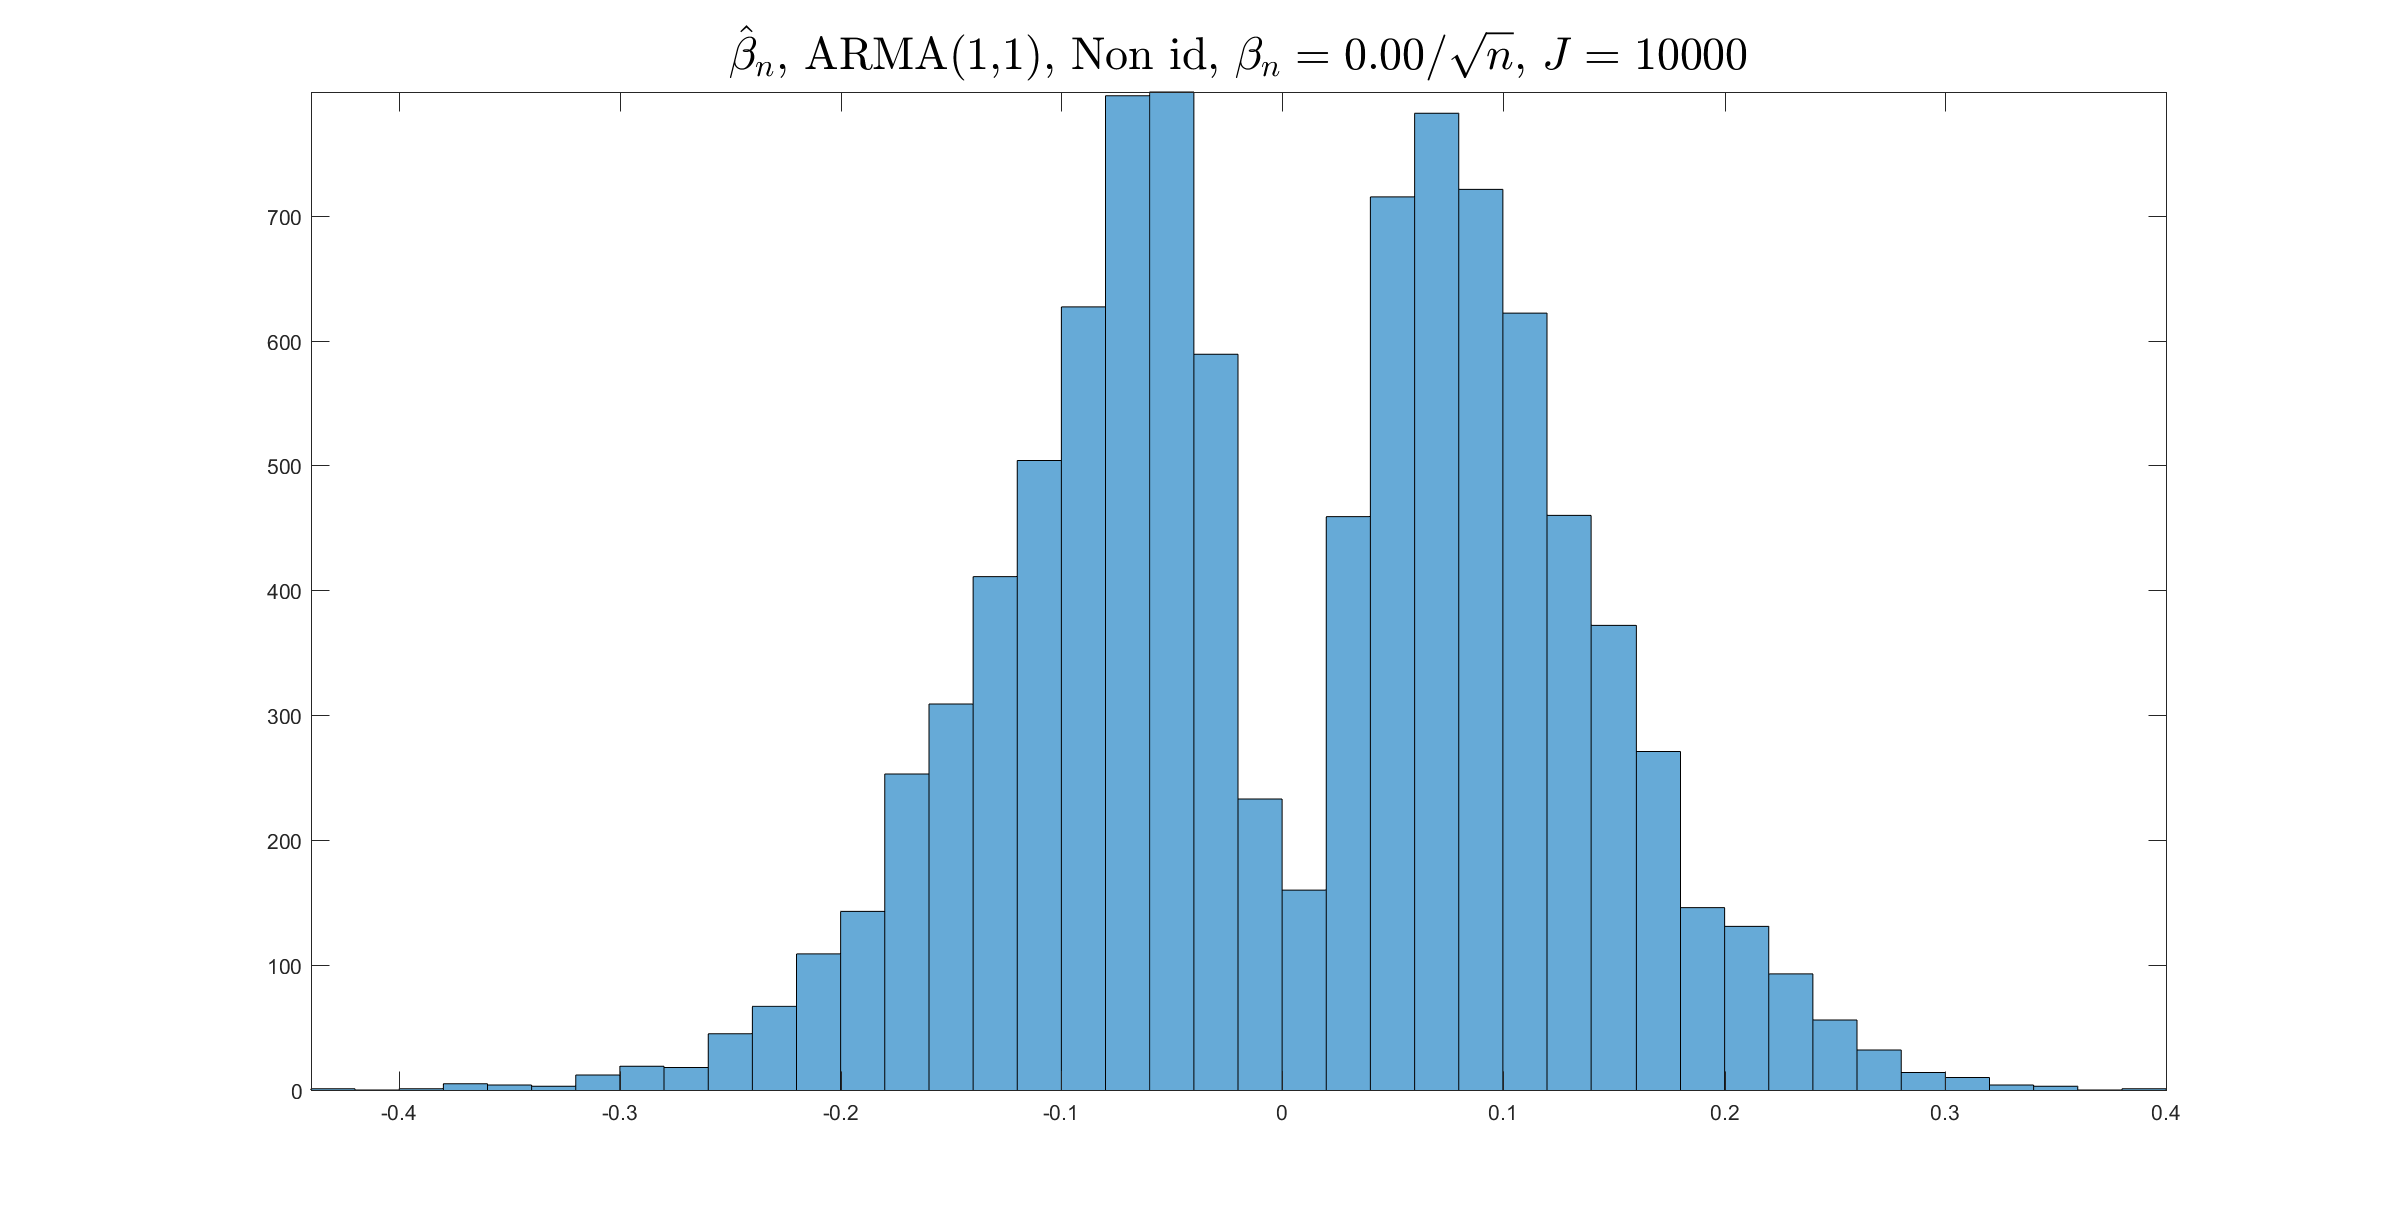
\includegraphics[scale=.3]{../fig/ARMA_beta_hat_id0_J10000.png}

$\Rightarrow$ Non-standard Inference!
\hfill 
\hyperlink{ARMA_beta_hat_id1}{\beamergotobutton{back to ARMA(1,1) $\hat{\beta}_{n}$}}
}


\frame[label = STAR_beta_hat_id1]{
\frametitle{Identification Robustness}
%Identification failure leads to non-standard asymptotic and finite sample distributions 
$y_t = \beta_n g(y_{t-1},\pi) + \zeta_n y_{t-1} + \e_{t}$:

\vspace*{.5cm}
\includegraphics[scale=.145]{../fig/STAR_beta_hat_id1_J10000.png}
\includegraphics[scale=.145]{../fig/STAR_beta_hat_id2_J10000.png}

\vspace*{.25cm}
\begin{itemize}
\item $\Rightarrow$ Non-standard Inference!
\hfill 
\hyperlink{ARMA_beta_hat_id1}{\beamergotobutton{ARMA(1,1) $\hat{\beta}_{n}$}}
\hyperlink{STAR_beta_hat_id0}{\beamergotobutton{STAR(1) $\hat{\beta}_{n}$, non-id}}


\vspace*{.25cm}
\item Current inference relies on calculation of distributions \citep{AndrewsPloberger1996,AndrewsCheng2012,Cheng2015}

\item Bootstrap has not been explored as a means of better approximating the finite sample distribution

%\item Any test statistic we want to bootstrap will involve these non-standard 
\end{itemize}

}



\frame[label = STAR_beta_hat_id0]{
\frametitle{Identification Robustness}
Identification failure leads to non-standard finite sample distributions ($y_t = \beta_n g(y_{t-1},\pi) + \zeta_n + \e_{t}$):

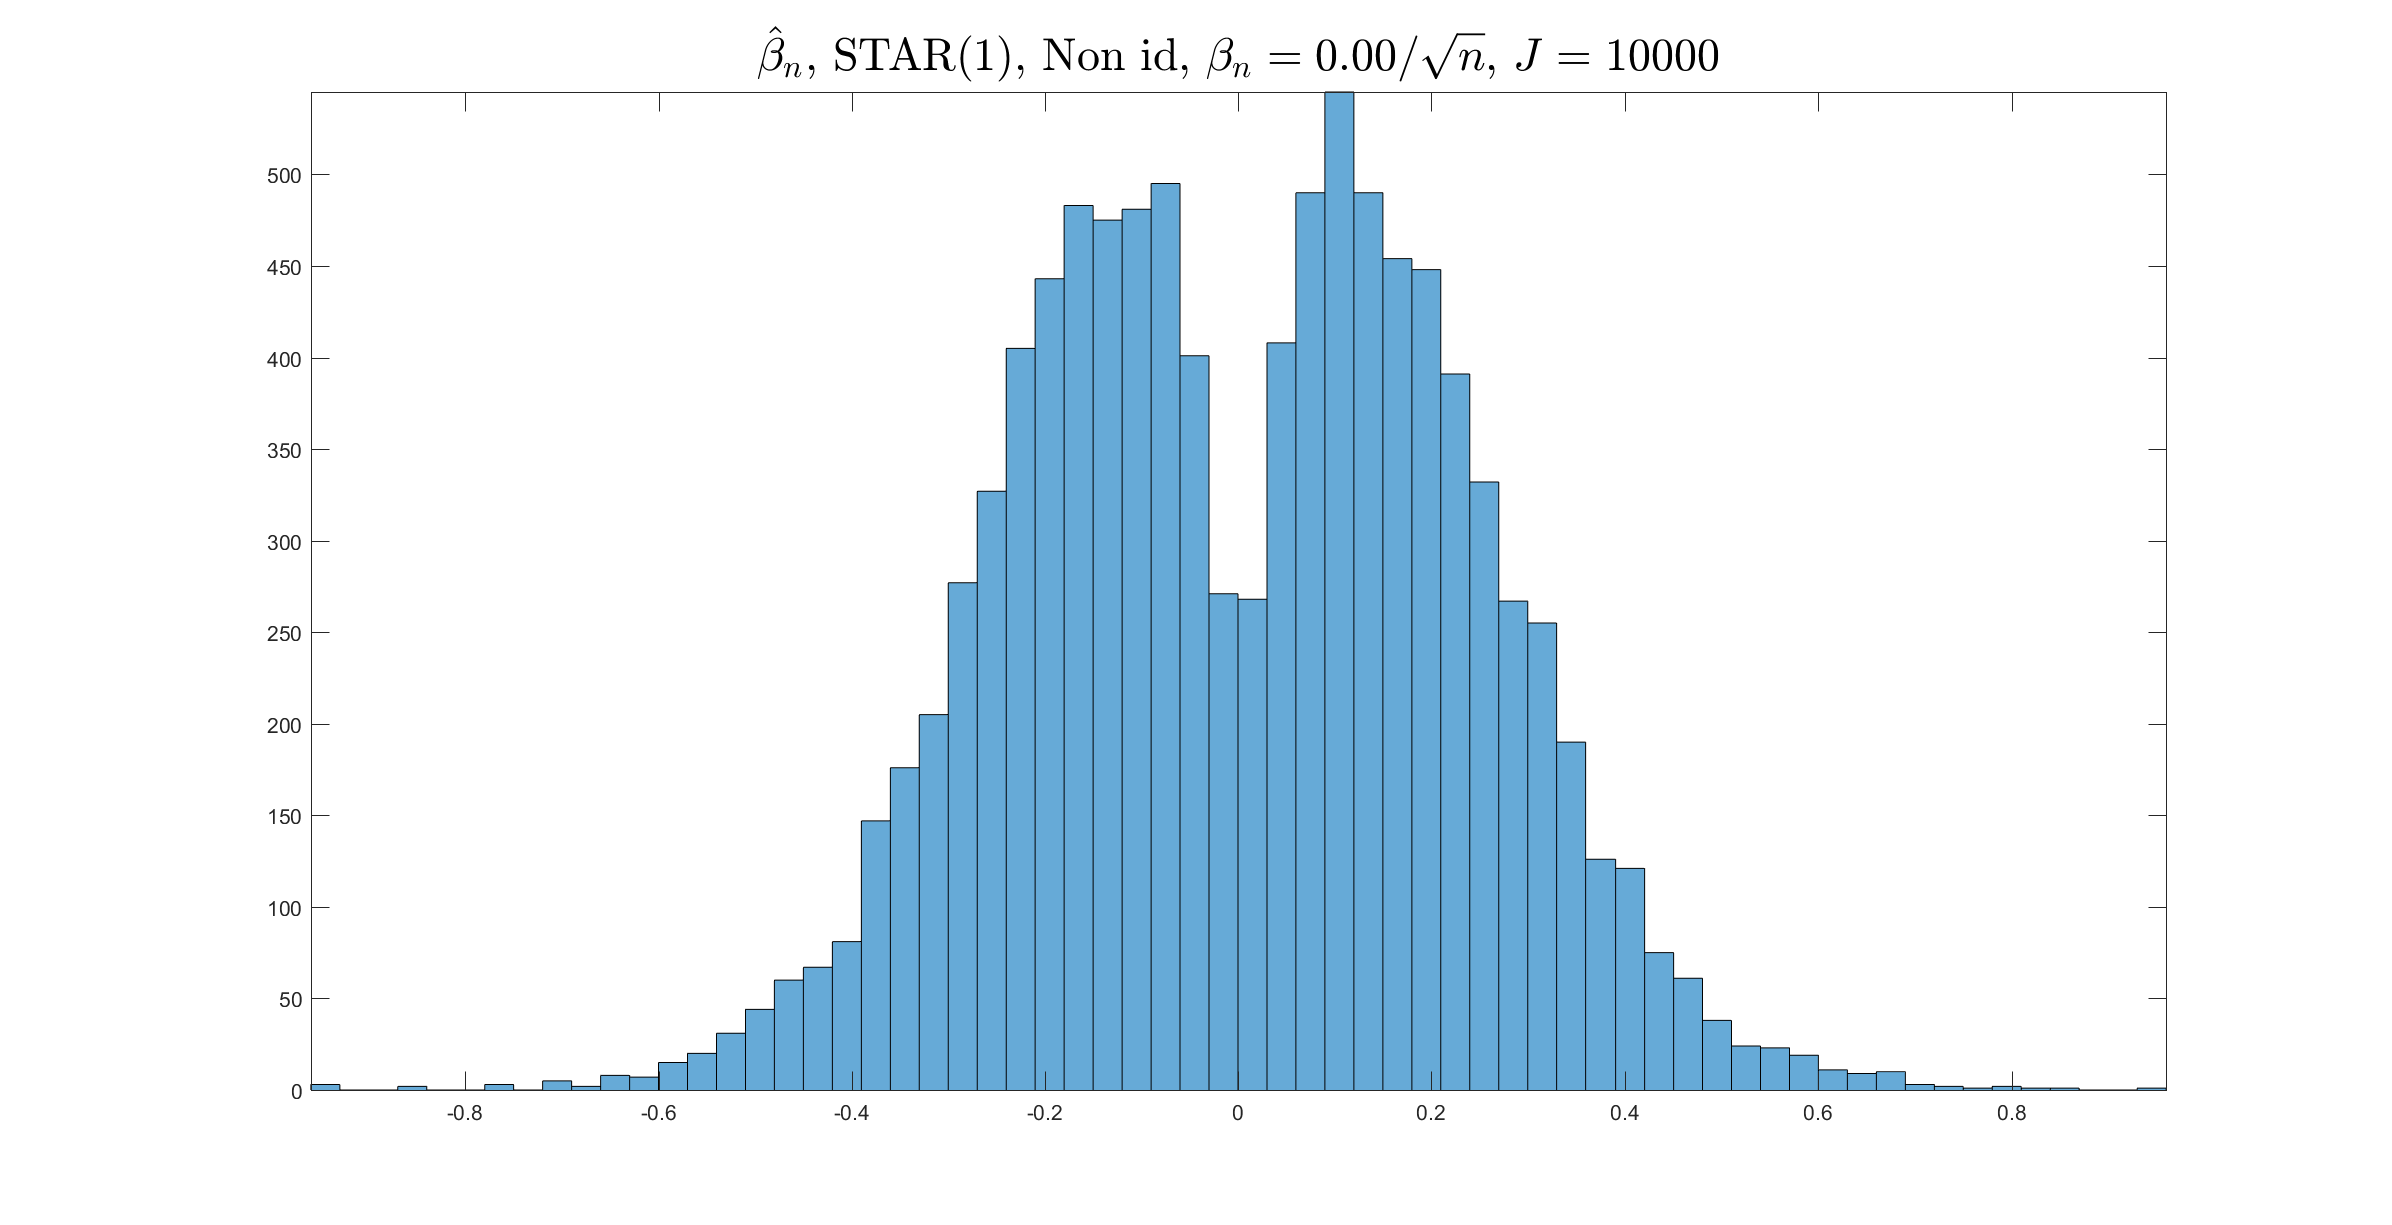
\includegraphics[scale=.3]{../fig/STAR_beta_hat_id0_J10000.png}

$\Rightarrow$ Non-standard Inference!
\hfill 
\hyperlink{STAR_beta_hat_id1}{\beamergotobutton{back to STAR(1) $\hat{\beta}_{n}$}}
}








\frame[label = beta_n_details]{
\frametitle{Identification Categories}
\begin{equation*}
n^{\alpha} \beta_{n} \to b \in \R^{k_{\beta}}
\end{equation*}

\vspace*{1cm}
\centering
\begin{tabular}[H]{cc}
$\alpha$ & Identification Category of $\pi$ \\
\hline
$\alpha \in [0,1/2)$ & (semi-) Strong \\
$\alpha \in [1/2,\infty)$ & Weak \\
\hline
\end{tabular}

\vspace*{1cm}
\hfill 
\hyperlink{weak_id_introduction}{\beamergotobutton{Return to Introduction}}
}




\frame[label = STAR_Assumptions]{
\frametitle{LSTAR Model Assumptions}
\begin{enumerate}[a]
\item True Parameter Space 
\begin{enumerate}[i]
\item $\Theta^* = \{(\beta, \zeta, \pi): \beta \in \B^*, \ \zeta \in \Z^*(\beta), \pi \in \Pi^*\}$ is compact.
\item $0 \in int(\B^*)$, $\Pi^* = \{ (\pi_1, \pi_2): \ \pi_1 \ge c\}$ for some $c>0$.  For some set $\Z_0^*$ and $\delta>0$, $\Z^*(\beta) = Z_0^*$ $\forall \beta$ s.t. $||\beta||<\delta$.
\end{enumerate}

\item Optimization Parameter Space 
\begin{enumerate}[i]
\item $\Theta = \{(\beta, \zeta, \pi): \beta \in \B, \ \zeta \in \Z(\beta), \pi \in \Pi\}$ is compact, and $\Theta^* \subset int(\Theta)$.
\item For some set $\Z_0$ and $\delta>0$, $\Z(\beta) = Z_0$ $\forall \beta$ s.t. $||\beta||<\delta$, and $\Z_0^* \subset int(\Z_0)$.
\end{enumerate}
\end{enumerate}

\hyperlink{STAR_Assumptions}{\beamergotobutton{Assumptions continued...}}
\hfill \hyperlink{STAR_Example}{\beamergotobutton{Return to LSTAR}}
}


\frame[label = STAR_Assumptions_2]{
\frametitle{LSTAR Model Assumptions}
\begin{enumerate}[a]
\setcounter{enumi}{2}
\item Under $H_0$, $E(\e_t| x_t) = 0$ a.s. and $E(\e_t^2|x_t) = \sigma^2 \in (0,\infty)$ a.s.

\item $E[\e_t(\psi_0,\pi) d_{\psi,t}(\pi)] = 0$ for a unique $\psi_0 = (0', \zeta_0')' \in int(\Psi^*)$, or $E[\e_t(\theta_0) d_{\theta,t}(\pi)] = 0$ for a unique $\theta_0 = (\beta_0', \zeta_0', \pi_0')' \in int(\Psi^* \times \Pi^*) = int(\Theta^*)$.

\item $y_t$ is strictly stationary, $L_p$-bounded for some $p>8$, and $\beta$-mixing with mixing coefficients $\beta_{l} = O(l^{-1p(1-p)-\iota})$ for some $q>p$ and $\iota>0$.

\item $g(\cdot, \pi)$ is Borel measurable for each $\pi$ and twice continuously differentiable in $\pi$.  $g(z_t, \pi)$ is a non-degenerate random variable for each $\pi \in \Pi$.  $E[\sup_{\pi \in \Pi} || (\partial/\partial \pi)^j g(z_t,\pi) ||^8] < \infty$ for $j = 0,1,2$.

\item Long Run Variances
\begin{enumerate}[i]
\item Under weak identification, $\liminf_{n\to \infty} \inf_{\alpha, r, \pi} E[(r' \sum_{i=1}^{m} \alpha_i G^{\psi}_{n}(\pi_i))^2] > 0$.
\item Under strong identification, $\liminf_{n\to \infty} \inf_{r} E[(r' G^{\theta}_{n})^2] > 0$.
\item $\inf_{r,\pi} E[(r' d_{\psi,t}(\pi))^2] > 0$ and $\inf_{r,\beta,\pi} E[(r' B^{-1}(\beta) d_{\theta,t}(\pi))^2] > 0$.
\end{enumerate}
\end{enumerate}

\hfill \hyperlink{STAR_Example}{\beamergotobutton{Return to LSTAR}}
}




\frame[label = Estimator_limits]{
\frametitle{Estimator Limiting Distributions}
Under \textbf{Weak Identification}:
\begin{equation*}
\pmat{n^{1/2}(\hat{\psi}_n - \psi_n) \\ \hat{\pi}_n} \tod \pmat{\T(\pi^*(\gamma_0, b); \gamma_0,b) \\ \pi^*(\gamma_0, b)}
\end{equation*}
where
\begin{itemize} \small
\item $\T(\pi; \gamma_0, b) = -H^{-1}(\pi; \gamma_0)(G(\pi; \gamma_0) + K(\pi; \gamma_0)b) - (b,0)$
\item $\pi^*(\gamma_0, b) = \argmin_{\pi \in \Pi} \xi(\pi; \gamma_0, b)$
\item and
$\xi(\pi; \gamma_0, b) = -\frac{1}{2} (G(\pi) + K(\pi, \pi_0)b)' H^{-1}(\pi) (G(\pi) + K(\pi, \pi_0)b)$.
\end{itemize}
\hfill \hyperlink{weak_id_objects}{\beamergotobutton{Weak ID Objects}}

\vspace*{.3cm}
Under \textbf{Strong Identification}:
\begin{equation*}
n^{1/2}B(\beta_n)(\hat{\theta}_n - \theta_n) \tod J^{-1} G^{\theta}
\end{equation*}
\begin{itemize} \small
\item where $B(\beta) = \pmat{I_{d_{\psi}} & 0_{d_{\psi} \times d_{\pi}} \\ 0_{d_{\psi} \times d_{\pi}} & ||\beta|| \cdot I_{d_{\pi}}}$ and 
$G^{\theta} \sim N(0,V)$
\end{itemize}

\hfill \hyperlink{STAR_Example}{\beamergotobutton{Return to LSTAR}}
}




\frame[label = weak_id_objects]{
\frametitle{LSTAR Model - Weak Identification Objects}
Define $d_{\psi, t}(\pi) = \deriv{\psi} \e_t(\psi, \pi) = (X_t' g(Z_t, \pi), X_t')'$.

\vspace*{.5cm}
$G(\cdot;\gamma_0)$ is a mean-zero Gaussian process with covariance kernel 
\begin{equation*}
\Omega(\pi, \tilde{\pi}; \gamma_0) = E_{\gamma_0} [\e_t^2 d_{\psi, t}(\pi)  d_{\psi, t}(\tilde{\pi})']
\end{equation*}
and
\begin{align*}
K(\pi; \gamma_0) &= -E_{\gamma_0}[ d_{\psi, t}(\pi) d_{\psi, t}(\pi_0)' \cdot S_{\beta}'], \qquad
S_{\beta} = [I_{d_{\beta}}: 0] \in \R^{d_{\beta} \times d_{\psi}}\\
H(\pi; \gamma_0) &= E_{\gamma_0}[ d_{\psi, t}(\pi) d_{\psi, t}(\pi)'] \\
D^{\psi}(h,\pi) &= E_{\gamma_0}[d_{\psi, t}(\pi) \e_{t-h}(\psi_{0,n},\pi) + d_{\psi, t-h}(\pi) \e_{t}(\psi_{0,n},\pi)]
\end{align*}
\hyperlink{Estimator_limits}{\beamergotobutton{Return to Estimator Limiting Distributions}}
\hfill \hyperlink{Test_stat_limiting_distribution}{\beamergotobutton{Return to Test Statistic Limiting Distributions}}
}


\frame[label = weak_id_objects_sample]{
\frametitle{LSTAR Sample Weak Identification Objects}
\begin{align*}
& \hat{H}_{n}(\pi) = \frac{1}{n} \sum_{t=1}^{n} d_{\psi, t}(\pi) d_{\psi, t}(\pi)' \\
& \hat{K}_{n}(\pi; \gamma_0) = -\frac{1}{n} \sum_{t=1}^{n} d_{\psi, t}(\pi) x_{t} g(z_t,\pi_0)
\end{align*}
and
\begin{align*}
G_{n}(\pi) 
&\equiv \frac{1}{\sqrt{n}} \sum_{t=1}^{n} \Big\{ m_{t}^{\psi}(\pi) - E_{\gamma_n}[m_{t}^{\psi}(\pi)] \Big\} \\
& m_{t}^{\psi}(\pi) \equiv m_{t}(\psi_{0,n},\pi) = \e_{t}(\psi_{0,n},\pi) d_{\psi,t}(\pi)
\end{align*}

\hyperlink{Estimator_limits}{\beamergotobutton{Return to Estimator Limiting Distributions}}
\hfill \hyperlink{Test_stat_limiting_distribution}{\beamergotobutton{Return to Test Statistic Limiting Distributions}}
}



\frame[label = Test_stat_limiting_distribution]{
\frametitle{Test Statistic Limits}

$\{ \Z^{\psi}(h, \pi): h \in \N, \pi \in \Pi\}$ is a 
\begin{itemize}
\item Gaussian process with mean $\lim\limits_{n\to \infty} \sqrt{n} E_{\gamma_n}(r^{2,\psi,n}_{t}(h,\pi)) < \infty$ and \item covariance kernel $\lim\limits_{n \to \infty} \frac{1}{n} \sum_{s,t=1}^{n}$ $E_{\gamma_n}[r^{1,\psi,n}_s(h, \pi)$ $r^{1,\psi,n}_t(\tilde{h}, \tilde{\pi})]$.  
\item where $r^{1,\psi,n}_t(h, \pi) = \frac{\e_{t} \e_{t-h} - E[\e_{t} \e_{t-h}]}{E[\e_{t}^2]} - \frac{ \D(h,\pi)' H^{-1}(\pi; \gamma_0) \big( m^{\psi}_t(\pi) - E_{\gamma_n}[m^{\psi}_t(\pi)] \big)}{E[\e_{t}^2]} $ and  
\item $r^{2,\psi,n}_t(h, \pi) = \frac{\e_{t}(\psi_{0,n}, \pi) \e_{t-h}(\psi_{0,n}, \pi) - \e_{t} \e_{t-h}}{E[\e_{t}^2]} - \frac{ \D(h,\pi)' H^{-1}(\pi; \gamma_0) \big( \beta_n \deriv{\tilde{\beta}} E_{\tilde{\gamma}_{n}}[m^{\psi}_t(\pi)] \big)}{E[\e_{t}^2]} $.
\end{itemize}

$\{ \Z^{\theta}(h): h \in \N\}$ is a 
\begin{itemize}
\item zero mean Gaussian process with
\item covariance kernel $\lim\limits_{n \to \infty} \frac{1}{n} \sum_{s,t=1}^{n} E[r^{\theta}_s(h) r^{\theta}_t(\tilde{h})]$.
\item where $r^{\theta}_t(h) = \frac{\e_{t} \e_{t-h} - E[\e_{t} \e_{t-h}] - \D^{\theta}(h)' J^{-1}(\gamma_0) m^{\theta}_t}{E[\e_{t}^2]}$.
\end{itemize}

\hyperlink{weak_id_objects}{\beamergotobutton{Go to LSTAR Weak ID Objets}}
\hfill
\hyperlink{Test_stat_theorem}{\beamergotobutton{Return to Test Statistics}}
}






\frame[label = bootstrap_algorithm_weak_id]{
\frametitle{Bootstrap under Weak Identification - Algorithm}
\textbf{Step 1.} Compute
{\small 
\begin{align*}
\hat{H}_n(\pi) & = \frac{1}{n} \sum_{t=1}^{n} d_{\psi, t}(\pi) d_{\psi, t}(\pi)' \\
\hat{K}_n(\pi; \gamma_0) & = \frac{1}{n} \sum_{t=1}^{n} d_{\psi, t}(\pi) x_t' g(z_t, \pi_0) \\
\hat{G}_{n}^{(bs)}(\pi) 
&= \frac{1}{\sqrt{n}} \sum_{t=1}^{n} z_t \Big\{ d_{\psi, t}(\pi) \e_t(\hat{\psi}_{\highlight{0,n}}(\pi), \pi)
- \frac{1}{n} \sum_{t=1}^{n} \big[ d_{\psi, t}(\pi) \e_t(\hat{\psi}_{\highlight{0,n}}(\pi), \pi) \big] \Big\}
\end{align*}
}% 

Define
\begin{align*}
& \xi_n^{(bs)}(\pi; \gamma_0, b) = \\
& \qquad -\frac{1}{2} \Big( \hat{G}_{n}^{(bs)}(\pi) + \hat{K}_n(\pi; \gamma_0) b \Big)' (\hat{H}_n(\pi))^{-1} \Big( \hat{G}_{n}^{(bs)}(\pi) + \hat{K}_n(\pi; \gamma_0) b \Big),
\end{align*}
and compute $\pi^*_{(bs)}(\gamma_0, b) = \argmin_{\pi \in \Pi} \xi^{(bs)}_{n}(\pi; \gamma_0, b)$.
}


\frame{
\frametitle{Bootstrap under Weak Identification - Algorithm}
\textbf{Step 2.} Use $\pi^*_{(bs)}(\gamma_0, b)$ and $\hat{\psi}_{0,n} = (0',\hat{\zeta}_n')'$ to compute 
\begin{align*}
\G_n(\pi^*_{(bs)}) = (\hat{H}_n(\pi^*_{(bs)}))^{-1} \Big[ m_{t}(\hat{\psi}_{0,n}, \pi^*_{(bs)}) - \frac{1}{n} \sum_{t=1}^{n} m_{t}(\hat{\psi}_{0,n}, \pi^*_{(bs)}) \Big]
\end{align*}
and 
\begin{align*}
& \hat{\D}_{n}(h, \pi^*_{(bs)}) = \\
& \frac{1}{n} \sum_{t=1+h}^{n} [d_{\psi, t}(\pi^*_{(bs)}) \e_{t-h}(\hat{\psi}_{0,n},\pi^*_{(bs)}) + d_{\psi, t-h}(\pi^*_{(bs)}) \e_{t}(\hat{\psi}_{0,n},\pi^*_{(bs)})].
\end{align*}

Define 
\begin{align*}
\hat{\E}_{t,h}(\psi, \pi)
& = \e_{t}(\psi, \pi)\e_{t-h}(\psi, \pi) - \G_n(\pi^*_{(bs)})' \hat{\D}_{n}(h, \pi^*_{(bs)}) \\
& \qquad - \highlight{\frac{1}{n} \sum_{t=1+h}^{n} [\e_{t}(\psi, \pi)\e_{t-h}(\psi, \pi) - \e_{t}\e_{t-h}]},
\end{align*}
}

\frame{
\frametitle{Bootstrap under Weak Identification - Algorithm}
\textbf{Step 3.} Use the draws $\{z_t\}$ to define
\begin{align*}
\hat{\rho}_n^{(w)}(h; \gamma_n, b)
& = \frac{1}{n^{-1}\sum_{t=1}^{n} \e_t^2(\hat{\theta}_n)} \times \Bigg\{ \frac{1}{n} \sum_{t=1+h}^{n} z_t \Big( \hat{\E}_{t,h}(\hat{\psi}_{0,n}, \pi^*_{(bs)}) \\
& \hspace*{.5cm} - \frac{1}{n} \sum_{t=1+h}^{n} \hat{\E}_{t,h}(\hat{\psi}_{0,n}, \pi^*_{(bs)}) \Big) \\
& \hspace*{.5cm} - ((\hat{H}_n(\pi^*_{(bs)}))^{-1} \hat{K}_n(\pi; \gamma_n) \frac{b}{\sqrt{n}})' \hat{\D}_{n}(h, \pi^*_{(bs)}) \\
& \hspace*{.5cm} + \highlight{\frac{1}{n} \sum_{t=1+h}^{n} [\e_{t}(\hat{\psi}_{0,n},\pi) \e_{t-h}(\hat{\psi}_{0,n},\pi) - \e_{t} \e_{t-h}]} \Bigg\}.
\end{align*}

Define the bootstrapped test statistic 
\begin{align*}
\hat{\Tc}_n^{(w)}(\gamma_n, b) = \max_{1\le h \le \Le_n} |\sqrt{n} \ \hat{\rho}_n^{(w)}(h; \gamma_n, b)|
\end{align*}
}

\frame{
\frametitle{Bootstrap under Weak Identification - Algorithm}
%Observe that we subtract $E_{\gamma_n}[\e_{t}(\psi, \pi)\e_{t-h}(\psi, \pi)]$ from the component that will multiplied by the random variable $z_t$, and then add $E_{\gamma_n}[\e_{t}(\psi, \pi)\e_{t-h}(\psi, \pi)]$ after.  Recall that the distribution of the test statistic has mean $\lim\limits_{n\to \infty} \sqrt{n} E_{\gamma_n}[\e_{t}(\psi_{0,n}, \pi^*)\e_{t-h}(\psi_{0,n}, \pi^*)]$, hence the reason for adding the quantity after multiplication by $z_t$.  We must subtract the quantity prior to multiplication as failing to do so will bias the variance of the bootstrapped distribution, since the variance in the distribution of the test statistic is based on $\e_{t} \e_{t-h}$, but our critical values are constructed using $\e_{t}(\hat{\psi}_{0,n}, \hat{\pi}_n)\e_{t-h}(\hat{\psi}_{0,n}, \hat{\pi}_n)$.

%Critical value construction, which is based on order statistics of repeated draws of $\hat{\Tc}_n^{(w)}(\gamma_n, b)$, is defined below.  Observe that the bootstrapped test statistic is a function of the nuisance parameters $(\pi_n, b)$ which cannot be consistently estimated.  Therefore, we will define the $\alpha$-level critical value $c_{n, 1-\alpha}^{(w)} = \sup_{\pi_n, b} c_{n, 1-\alpha}^{(w)}(\gamma_n, b)$.

\textbf{Step 4.}  The final step is discussed under critical value computation.

\vspace{2cm}
\hyperlink{cv_computation}{\beamergotobutton{Go to Critical Value Computation}}
\hfill 
\hyperlink{bootstrap_summary_weak_id}{\beamergotobutton{Return to Bootstrap Summary}}
}


\subsubsection{Strong Identification}
\frame[label = bootstrap_algorithm_strong_id]{
\frametitle{Bootstrap under Strong Identification - Algorithm}

\begin{itemize}
\item Simpler construction (no bias terms)
\item Simpler procedure (no $\pi^*$ and no nuisance parameters).
\end{itemize}

\begin{enumerate}
\item Compute $\hat{J}_n(\hat{\theta}_n) = \frac{1}{n} \sum_{t=1}^{n} B(\hat{\beta}_n)^{-1}  d_{\theta, t}(\hat{\theta}_{n}) d_{\theta, t}(\hat{\theta}_{n})' B(\hat{\beta}_n)^{-1 \prime}$,  
$\hat{\D}^{\theta}_{n}(h, \hat{\theta}_n) = \frac{1}{n} \sum_{t=1+h}^{n} B(\hat{\beta}_n)^{-1}  [d_{\theta, t}(\hat{\theta}_{n}) \e_{t-h}(\hat{\theta}_{n}) + d_{\theta, t-h}(\hat{\theta}_{n}) \e_{t}(\hat{\theta}_{n})]$, and $m^{\theta}_t(\theta) = d_{\theta, t}(\hat{\theta}_{n}) \e_{t}(\hat{\theta}_{n})$.

\item Define $\hat{\E}_{t,h}(\theta) 
= \e_{t}(\theta)\e_{t-h}(\theta) - (\hat{\D}^{\theta}_{n}(h, \theta))' (\hat{J}_n(\hat{\theta}_n))^{-1} B(\hat{\beta}_n)^{-1} m^{\theta}_t(\theta)$.

\item Use the draws $\{z_t\}$ to define
\begin{align*}
\hat{\rho}_n^{(s)}(h)
& = \frac{1}{n^{-1}\sum_{t=1}^{n} \e_t^2(\hat{\theta}_n)} \\
& \qquad \times \Bigg\{ \frac{1}{n} \sum_{t=1+h}^{n} z_t \Big( \hat{\E}_{t,h}(\hat{\theta}_n)  - \frac{1}{n} \sum_{t=1+h}^{n} \hat{\E}_{t,h}(\hat{\theta}_n) \Big) \Bigg\}
\end{align*}

\item Define the bootstrapped test statistic $\hat{\Tc}_n^{(s)} = \max_{1\le h \le \Le_n} |\sqrt{n} \ \hat{\rho}_n^{(s)}(h)|$.
\end{enumerate}

\hyperlink{cv_computation}{\beamergotobutton{Go to Critical Value Computation}}
\hfill 
\hyperlink{bootstrap_summary_weak_id}{\beamergotobutton{Return to Bootstrap Summary}}
}




\frame[label = cv_computation]{
\frametitle{Critical Value Computation - Algorithm}
\begin{enumerate}
\item For $k = w,s$, repeat the above procedures $i=1,\dots, M$ times: $\{ \hat{\Tc}_{n,i}^{(s)} \}_{i=1}^{M}$ and $\{ \hat{\Tc}_{n,i}^{(w)}(\gamma_n, b) \}_{i=1}^{M}$.
\item Define the order statistics $\{ \hat{\Tc}_{n,(i)}^{(k)} \}_{i=1}^{M}$ such that $\hat{\Tc}_{n,(1)}^{(k)} \le \hat{\Tc}_{n,(2)}^{(k)} \le \cdots \le \hat{\Tc}_{n,(M)}^{(k)}$.
\item The approximate $\alpha$-level critical values are
\begin{itemize}
\item strong id: $\hat{c}_{n, 1-\alpha}^{(s)} = \hat{\Tc}_{n,[(1-\alpha)\cdot M]}^{(s)}$
\item weak id: $\hat{c}_{n, 1-\alpha}^{(w)}(\gamma_n, b) = \hat{\Tc}_{n,[(1-\alpha)\cdot M]}^{(w)}(\gamma_n, b)$
\begin{itemize}
\item Consistent estimators are not available for $(\pi_n, b)$
\item In practice, $c_{n, 1-\alpha}^{(w)} = \sup_{\pi_n, b} c_{n, 1-\alpha}^{(w)}(\gamma_n, b)$.
\end{itemize}
\end{itemize}
\end{enumerate}

\vspace{1cm}
\hyperlink{cv_computation_summary}{\beamergotobutton{Return to Critical Value Overview}}
\hfill 
\hyperlink{bootstrap_summary_weak_id}{\beamergotobutton{Return to Bootstrap Overview}}
}




\frame[label = ICS_cv_details]{
\frametitle{ICS Critical Values}
The statistic used for category selection is 
\begin{equation*}
\A_n = (n \hat{\beta}_n' \hat{\Sigma}_{\beta \beta, n}^{-1} \hat{\beta}_n / d_{\beta})^{1/2}
\end{equation*}
where $\hat{\Sigma}_{\beta \beta, n}$ is the upper left $d_{\beta} \times d_{\beta}$ block of $\hat{\Sigma}_{n} = \hat{J}_n^{-1} \hat{V}_n \hat{J}_n^{-1}$, the estimator of the strong identification covariance matrix $\Sigma(\gamma_0) = J^{-1} V J^{-1}$.

Let $\{\kappa_n: \ n\ge 1\}$ be a sequence of constants s.t. 
\begin{equation*}
\kappa_n \to \infty \qquad \text{and} \qquad \kappa_n / n^{1/2} \to 0
\end{equation*}

The ICS critical value is $c_{1-\alpha}^{(ICS)} = \begin{cases}
c_{1-\alpha}^{(LF)} & \qquad \text{if} \ \A_n \le \kappa_n \\ 
c_{1-\alpha}^{(s)} & \qquad \text{if} \ \A_n > \kappa_n
\end{cases}$

\hfill 
\hyperlink{robust_cvs}{\beamergotobutton{Return to CV Overview}}
}



\frame[label = slide_for_Valentin]{
\frametitle{Why not just test a Taylor Expansion of the model?}

\begin{itemize}
\item Some tests for linearity against STR alternatives use a Taylor expansion. (e.g. \citep{Luukkonen_etal1988}).
\item This adds a remainder term to the error.
\item Taylor Expansion of $g(z,\pi)$ around $\pi_{1} = 0$ (not $\pi_{1,0}$):
\begin{align*}
y_{t} = \zeta y_{t-1} + \beta y_{t-1} g(z_{t},\pi) + \e_t
\quad \Rightarrow \quad
y_{t} & = \alpha_{0} y_{t-1} + \alpha_{1} y_{t-1} z_{t} + \nu_{t} \\
& \nu_{t} = \e_{t} + \beta y_{t-1} R(z_{t}, \pi) 
\end{align*}

\item $H_0$ says nothing about $\beta$ or $\pi$ $\Rightarrow$ $E[\nu_{t}\nu_{t-h}] \ne 0$.
\hfill 
\hyperlink{slide_for_Valentin_adendum}{\beamergotobutton{Adendum}}

\item Future Questions:
\begin{itemize}
\item Longer Expansion: must make $R(z_t, \pi)$ and $R(z_t, \pi)^2$ disappear
\item What about other models (e.g. ARMA)? 
\end{itemize}
\end{itemize}

\vfill
\hyperlink{introduction_white_noise_test}{\beamergotobutton{Return to Introduction}}
\hfill 
\hyperlink{white_noise_test_recap}{\beamergotobutton{Return to White Noise Test Recap}}
}



\frame[label = slide_for_Valentin_adendum]{
\frametitle{Adendum to Taylor Expansion method}

\begin{itemize}
\item Under non-identification, $\beta_n = 0$
\item Under weak identification $\beta_n \to 0$, $\sqrt{n} \beta_n \to b < \infty$
\end{itemize}
\begin{align*}
\text{Under } H_{0}, \quad
\sqrt{n} & E_{\gamma_{n}}[\nu_{t} \nu_{t-h}] \\
& = \sqrt{n} E[\e_{t} \e_{t-h}] + \sqrt{n} E_{\gamma_{n}}[\beta_{n} y_{t-1} \e_{t-h} R(z_{t}, \pi)] 
\\ & \qquad + \sqrt{n} E_{\gamma_{n}}[\beta_{n} y_{t-1-h} \e_{t} R(z_{t-h}, \pi)]
\\ & \qquad + \sqrt{n} E_{\gamma_{n}}[\beta_{n} y_{t-1} y_{t-1-h} R(z_{t}, \pi) \beta_{n}  R(z_{t-h}, \pi)] \\
% & \to b E[y_{t-1} \e_{t-h} R(z_{t}, \pi)] + b E[y_{t-1-h} \e_{t} R(z_{t-h}, \pi)] \\ & \qquad + \beta_{n} b E[ y_{t-1} y_{t-1-h} R(z_{t}, \pi) R(z_{t-h}, \pi)] \\
& \to b E[y_{t-1} \e_{t-h} R(z_{t}, \pi)] + b E[y_{t-1-h} \e_{t} R(z_{t-h}, \pi)]
\end{align*}
\begin{itemize}
\item Potential for new robust test:
\begin{itemize}
\item Use Taylor expansion under weak identification
\item Use original model under strong identification
\item eliminate the need to sup over nuisance parameters in practice
\item but still not clear how to use this method for other models...
\end{itemize}
\end{itemize}

\vfill
\hfill 
\hyperlink{slide_for_Valentin}{\beamergotobutton{Return to Taylor Expansion Page}}
}








%%%%%%%%%%%%%%%%%%%%%%%%
%%%%%%%%%%%%%%%%%%%%%%%%
%%%%%%%%%%%%%%%%%%%%%%%%
%%%%%%%%%%%%%%%%%%%%%%%%
%%%%%%%%%%%%%%%%%%%%%%%%
%%%%%%%%%%%%%%%%%%%%%%%%
%%%%%%%%%%%%%%%%%%%%%%%%
%%%%%%%%%%%%%%%%%%%%%%%%
%%%%%%%%%%%%%%%%%%%%%%%%
%%%%%%%%%%%%%%%%%%%%%%%%
%%%%%%%%%%%%%%%%%%%%%%%%%%%%%%%%%%%%%%%%%%%%%%%%
%%%%%%%%%%%%%%%%%%%%%%%%
%%%%%%%%%%%%%%%%%%%%%%%%
%%%%%%%%%%%%%%%%%%%%%%%%
%%%%%%%%%%%%%%%%%%%%%%%%
%%%%%%%%%%%%%%%%%%%%%%%%
%%%%%%%%%%%%%%%%%%%%%%%%
%%%%%%%%%%%%%%%%%%%%%%%%
%%%%%%%%%%%%%%%%%%%%%%%%
%%%%%%%%%%%%%%%%%%%%%%%%
%%%%%%%%%%%%%%%%%%%%%%%%%%%%%%%%%%%%%%%%%%%%%%%%
%%%%%%%%%%%%%%%%%%%%%%%%
%%%%%%%%%%%%%%%%%%%%%%%%
%%%%%%%%%%%%%%%%%%%%%%%%
%%%%%%%%%%%%%%%%%%%%%%%%
%%%%%%%%%%%%%%%%%%%%%%%%
%%%%%%%%%%%%%%%%%%%%%%%%
%%%%%%%%%%%%%%%%%%%%%%%%
%%%%%%%%%%%%%%%%%%%%%%%%
%%%%%%%%%%%%%%%%%%%%%%%%
%%%%%%%%%%%%%%%%%%%%%%%%%%%%%%%%%%%%%%%%%%%%%%%%
%%%%%%%%%%%%%%%%%%%%%%%%
%%%%%%%%%%%%%%%%%%%%%%%%
%%%%%%%%%%%%%%%%%%%%%%%%
%%%%%%%%%%%%%%%%%%%%%%%%
%%%%%%%%%%%%%%%%%%%%%%%%
%%%%%%%%%%%%%%%%%%%%%%%%
%%%%%%%%%%%%%%%%%%%%%%%%
%%%%%%%%%%%%%%%%%%%%%%%%
%%%%%%%%%%%%%%%%%%%%%%%%
%%%%%%%%%%%%%%%%%%%%%%%%%%%%%%%%%%%%%%%%%%%%%%%%
%%%%%%%%%%%%%%%%%%%%%%%%
%%%%%%%%%%%%%%%%%%%%%%%%
%%%%%%%%%%%%%%%%%%%%%%%%
%%%%%%%%%%%%%%%%%%%%%%%%
%%%%%%%%%%%%%%%%%%%%%%%%
%%%%%%%%%%%%%%%%%%%%%%%%
%%%%%%%%%%%%%%%%%%%%%%%%
%%%%%%%%%%%%%%%%%%%%%%%%
%%%%%%%%%%%%%%%%%%%%%%%%
%%%%%%%%%%%%%%%%%%%%%%%%



\backupend



% % % % % % % % % % % % % % % % % % % % % % % % % % % % % % % % % % % % % % % % % % %
% % % % % % % % % % % % % % % % % % % % % % % % % % % % % % % % % % % % % % % % % % % % % % %
% % % % % % % % % % % % % % % % % % % % % % % % % % % % % % % % % % % % % % % % % %
% % % % % % % % % % % % % % % % % % % % % % % % % % % % % % % % % % % % % % % % % % % % % %
% % % % % % % % % % % % % % % % % % % % % % % % % % % % % % % % % % % % % % % % % % % % % %
% % % % % % % % % % % % % % % % % % % % % % % % % % % % % % % % % % % % % % % % % % % % % %
% % % % % % % % % % % % % % % % % % % % % % % % % % % % % % % % % % % % % % % % % % % % % %
% % % % % % % % % % % % % % % % % % % % % % % % % % % % % % % % % % % % % % % % % % % % % %
% % % % % % % % % % % % % % % % % % % % % % % % % % % % % % % % % % % % % % % % % % % % % %
% % % % % % % % % % % % % % % % % % % % % % % % % % % % % % % % % % % % % % % % % % % % % %


\frame[label=slide_label]{

\hyperlink{slide_label}{\beamergotobutton{Go Back.}}
}



\begin{itemize}
\small
\setlength{\itemsep}{0cm}%
\setlength{\parskip}{0cm}%
\item 
\end{itemize}

\frame{
\frametitle{}
\begin{columns}[onlytextwidth]
\begin{column}{0.5\textwidth}
\centering
%\includegraphics[scale=.22]{two_dogsA}
\end{column}

\begin{column}{0.5\textwidth}
\centering
%\includegraphics[scale=.22]{two_dogsB}
\end{column}
\end{columns}
}





